\documentclass[twoside,nohyper]{tufte-book}
\makeatletter\let\tufte@caption\@caption\makeatother
% ams
\usepackage{amssymb,amsmath}

\usepackage{ifxetex,ifluatex}
\usepackage{fixltx2e} % provides \textsubscript
\ifnum 0\ifxetex 1\fi\ifluatex 1\fi=0 % if pdftex
  \usepackage[T1]{fontenc}
  \usepackage[utf8]{inputenc}
\else % if luatex or xelatex
  \makeatletter
  \@ifpackageloaded{fontspec}{}{\usepackage{fontspec}}
  \makeatother
  \defaultfontfeatures{Ligatures=TeX,Scale=MatchLowercase}
  \makeatletter
  \@ifpackageloaded{soul}{
     \renewcommand\allcapsspacing[1]{{\addfontfeature{LetterSpace=15}#1}}
     \renewcommand\smallcapsspacing[1]{{\addfontfeature{LetterSpace=10}#1}}
   }{}
  \makeatother

\fi

% graphix
\usepackage{graphicx}
\setkeys{Gin}{width=\linewidth,totalheight=\textheight,keepaspectratio}

% booktabs
\usepackage{booktabs}

% url
\usepackage{url}

% hyperref
\usepackage{hyperref}\makeatletter\let\@caption\tufte@caption\makeatother

% units.
\usepackage{units}


\setcounter{secnumdepth}{2}

% citations
\usepackage{natbib}
\bibliographystyle{abbrvnat}

% pandoc syntax highlighting
\usepackage{color}
\usepackage{fancyvrb}
\newcommand{\VerbBar}{|}
\newcommand{\VERB}{\Verb[commandchars=\\\{\}]}
\DefineVerbatimEnvironment{Highlighting}{Verbatim}{commandchars=\\\{\}}
% Add ',fontsize=\small' for more characters per line
\newenvironment{Shaded}{}{}
\newcommand{\AlertTok}[1]{\textcolor[rgb]{1.00,0.00,0.00}{\textbf{#1}}}
\newcommand{\AnnotationTok}[1]{\textcolor[rgb]{0.38,0.63,0.69}{\textbf{\textit{#1}}}}
\newcommand{\AttributeTok}[1]{\textcolor[rgb]{0.49,0.56,0.16}{#1}}
\newcommand{\BaseNTok}[1]{\textcolor[rgb]{0.25,0.63,0.44}{#1}}
\newcommand{\BuiltInTok}[1]{#1}
\newcommand{\CharTok}[1]{\textcolor[rgb]{0.25,0.44,0.63}{#1}}
\newcommand{\CommentTok}[1]{\textcolor[rgb]{0.38,0.63,0.69}{\textit{#1}}}
\newcommand{\CommentVarTok}[1]{\textcolor[rgb]{0.38,0.63,0.69}{\textbf{\textit{#1}}}}
\newcommand{\ConstantTok}[1]{\textcolor[rgb]{0.53,0.00,0.00}{#1}}
\newcommand{\ControlFlowTok}[1]{\textcolor[rgb]{0.00,0.44,0.13}{\textbf{#1}}}
\newcommand{\DataTypeTok}[1]{\textcolor[rgb]{0.56,0.13,0.00}{#1}}
\newcommand{\DecValTok}[1]{\textcolor[rgb]{0.25,0.63,0.44}{#1}}
\newcommand{\DocumentationTok}[1]{\textcolor[rgb]{0.73,0.13,0.13}{\textit{#1}}}
\newcommand{\ErrorTok}[1]{\textcolor[rgb]{1.00,0.00,0.00}{\textbf{#1}}}
\newcommand{\ExtensionTok}[1]{#1}
\newcommand{\FloatTok}[1]{\textcolor[rgb]{0.25,0.63,0.44}{#1}}
\newcommand{\FunctionTok}[1]{\textcolor[rgb]{0.02,0.16,0.49}{#1}}
\newcommand{\ImportTok}[1]{#1}
\newcommand{\InformationTok}[1]{\textcolor[rgb]{0.38,0.63,0.69}{\textbf{\textit{#1}}}}
\newcommand{\KeywordTok}[1]{\textcolor[rgb]{0.00,0.44,0.13}{\textbf{#1}}}
\newcommand{\NormalTok}[1]{#1}
\newcommand{\OperatorTok}[1]{\textcolor[rgb]{0.40,0.40,0.40}{#1}}
\newcommand{\OtherTok}[1]{\textcolor[rgb]{0.00,0.44,0.13}{#1}}
\newcommand{\PreprocessorTok}[1]{\textcolor[rgb]{0.74,0.48,0.00}{#1}}
\newcommand{\RegionMarkerTok}[1]{#1}
\newcommand{\SpecialCharTok}[1]{\textcolor[rgb]{0.25,0.44,0.63}{#1}}
\newcommand{\SpecialStringTok}[1]{\textcolor[rgb]{0.73,0.40,0.53}{#1}}
\newcommand{\StringTok}[1]{\textcolor[rgb]{0.25,0.44,0.63}{#1}}
\newcommand{\VariableTok}[1]{\textcolor[rgb]{0.10,0.09,0.49}{#1}}
\newcommand{\VerbatimStringTok}[1]{\textcolor[rgb]{0.25,0.44,0.63}{#1}}
\newcommand{\WarningTok}[1]{\textcolor[rgb]{0.38,0.63,0.69}{\textbf{\textit{#1}}}}

% longtable
\usepackage{longtable,booktabs}

% multiplecol
\usepackage{multicol}

% strikeout
\usepackage[normalem]{ulem}

% morefloats
\usepackage{morefloats}


% tightlist macro required by pandoc >= 1.14
\providecommand{\tightlist}{%
  \setlength{\itemsep}{0pt}\setlength{\parskip}{0pt}}

% title / author / date
\title{Energy Efficiency in Wireless Communications for Mobile User Devices}
\author{Iñaki Úcar Marqués}
\date{2018-11-20}

\usepackage[hyperpageref]{backref}
\usepackage[nottoc]{tocbibind}
\usepackage{bibentry,bookmark,hyperxmp}
\usepackage{etoolbox,xstring}
\usepackage{algorithm,algpseudocode}
\usepackage{multirow,tabu,rotating}
\usepackage{parcolumns}
\usepackage{pdfpages}
%\usepackage{makeidx}
%\makeindex

\DeclareGraphicsExtensions{.pdf}

\hypersetup{
  pdfauthor         = {Iñaki Úcar Marqués},
  pdfcopyright      = {© The author. Some rights reserved. This document is under terms of Creative Commons license Attribution - Non Commercial - Non Derivatives.},
  pdflicenseurl     = {http://creativecommons.org/licenses/by-nc-nd/3.0/es/},
  pdfkeywords       = {Energy Efficiency, Wireless Networks, User Device},
  pdfsubject        = {Tesis doctoral. Universidad Carlos III de Madrid. Departamento de Ingeniería Telemática.},
  pdfencoding       = auto,
  bookmarksnumbered = true,
  bookmarksdepth    = 3,
  pdfborder         = {0 0 0},
  colorlinks        = true,
  citecolor         = DarkGreen,
  linkcolor         = DarkBlue,
  urlcolor          = DarkGreen
}

\renewcommand{\bibname}{References}
\def\HighlightName#1{\IfSubStr{#1}{Ucar}{\textbf{#1}}{#1}}
\renewcommand*{\backref}[1]{}
\renewcommand*{\backrefalt}[4]{\marginnote{\ifcase #1 No citations\or p. #2\else pp. #2\fi}}
\renewcommand*{\doi}[1]{\href{http://dx.doi.org/#1}{\smallcaps{DOI}: #1}}
\publisher{Universidad Carlos III de Madrid}
\definecolor{uc3m}{cmyk}{0.9827, 1, 0.2624, 0.1077}

% \RequirePackage[letterpaper,left=1in,top=1in,headsep=2\baselineskip,textwidth=26pc,marginparsep=2pc,marginparwidth=12pc,textheight=44\baselineskip,headheight=\baselineskip]{geometry}
% therefore, margins for letter paper are: 1 in left, 1-0.142 in right
\newcommand{\increaseinnermargin}{
  \setlength{\evensidemargin}{-0.242in} %twoside
  %\setlength{\evensidemargin}{\evensidemargin-0.1in} %symmetric
  \setlength{\oddsidemargin}{0.1in}
}
\increaseinnermargin

\newcommand{\restorefullwidth}{
  \newgeometry{
    left = 1in, top = 1in, headsep = 2\baselineskip,
    textwidth = 40pc, marginparsep = 0pc, marginparwidth = 0pc,
    textheight = 44\baselineskip, headheight = \baselineskip
  }
  \fancyhfoffset[RO]{0pt}
  \increaseinnermargin
}

\newcommand{\restorewidth}{
  \restoregeometry
  \fancyhfoffset[RO]{{\marginparsep+\marginparwidth}}
}

% patch part toc line; hackish, but it works: don't touch it
\makeatletter
\let\oldcontentsline\contentsline
\def\contentsline#1#2{%
  \expandafter\ifx\csname l@#1\endcsname\l@part
    \expandafter\@firstoftwo \else \expandafter\@secondoftwo \fi
  {\oldcontentsline{#1}{\allcaps{Part\quad#2}}}
  {\oldcontentsline{#1}{#2}}
}
\makeatother

\newcommand{\partseparator}{
  \noindent\leavevmode\leaders\hrule height 0.8ex depth \dimexpr0.4pt-0.8ex\hfill\kern0pt
  \newline~\vspace{-0.5\baselineskip}\newline}

\titlecontents{part}%
  [0pt]% distance from left margin
  {}{}{}{} % leave blank; the patch above does the rest
  [\vspace*{0.5\baselineskip}]% after

\titlecontents{chapter}%
  [4em]% distance from left margin
  {}% above (global formatting of entry)
  {\contentslabel{2em}\textit}% before w/ label (label = ``Chapter 1'')
  {\hspace{0em}\textit}% before w/o label
  {\qquad\thecontentspage}% filler and page (leaders and page num)
  [\vspace*{0.5\baselineskip}]% after

\titlecontents{section}%
  [6em]% distance from left margin
  {}% above (global formatting of entry)
  {\contentslabel{2em}\textit}% before w/ label (label = ``Chapter 1'')
  {\hspace{0em}\textit}% before w/o label
  {\qquad\thecontentspage}% filler and page (leaders and page num)
  [\vspace*{0.5\baselineskip}]% after

\titleformat{\part}%
  [block]% shape
  {\begin{fullwidth}}% format applied to label+text
  {\itshape\Huge\hfill \partname~\thepart}% label
  {0pt}% horizontal separation between label and title body
  {\Huge\rmfamily\itshape\quad}% before the title body
  [\end{fullwidth}]% after the title body

 \titleformat{\chapter}
  [block]% shape
  {\relax\ifthenelse{\NOT\boolean{@tufte@symmetric}}{\begin{fullwidth}}{}}% format applied to label+text
  {\itshape\huge\thechapter}% label
  {1em}% horizontal separation between label and title body
  {\huge\rmfamily\itshape}% before the title body
  [\ifthenelse{\NOT\boolean{@tufte@symmetric}}{\end{fullwidth}}{}]% after the title body

\makeatletter
\renewcommand{\maketitlepage}{%
  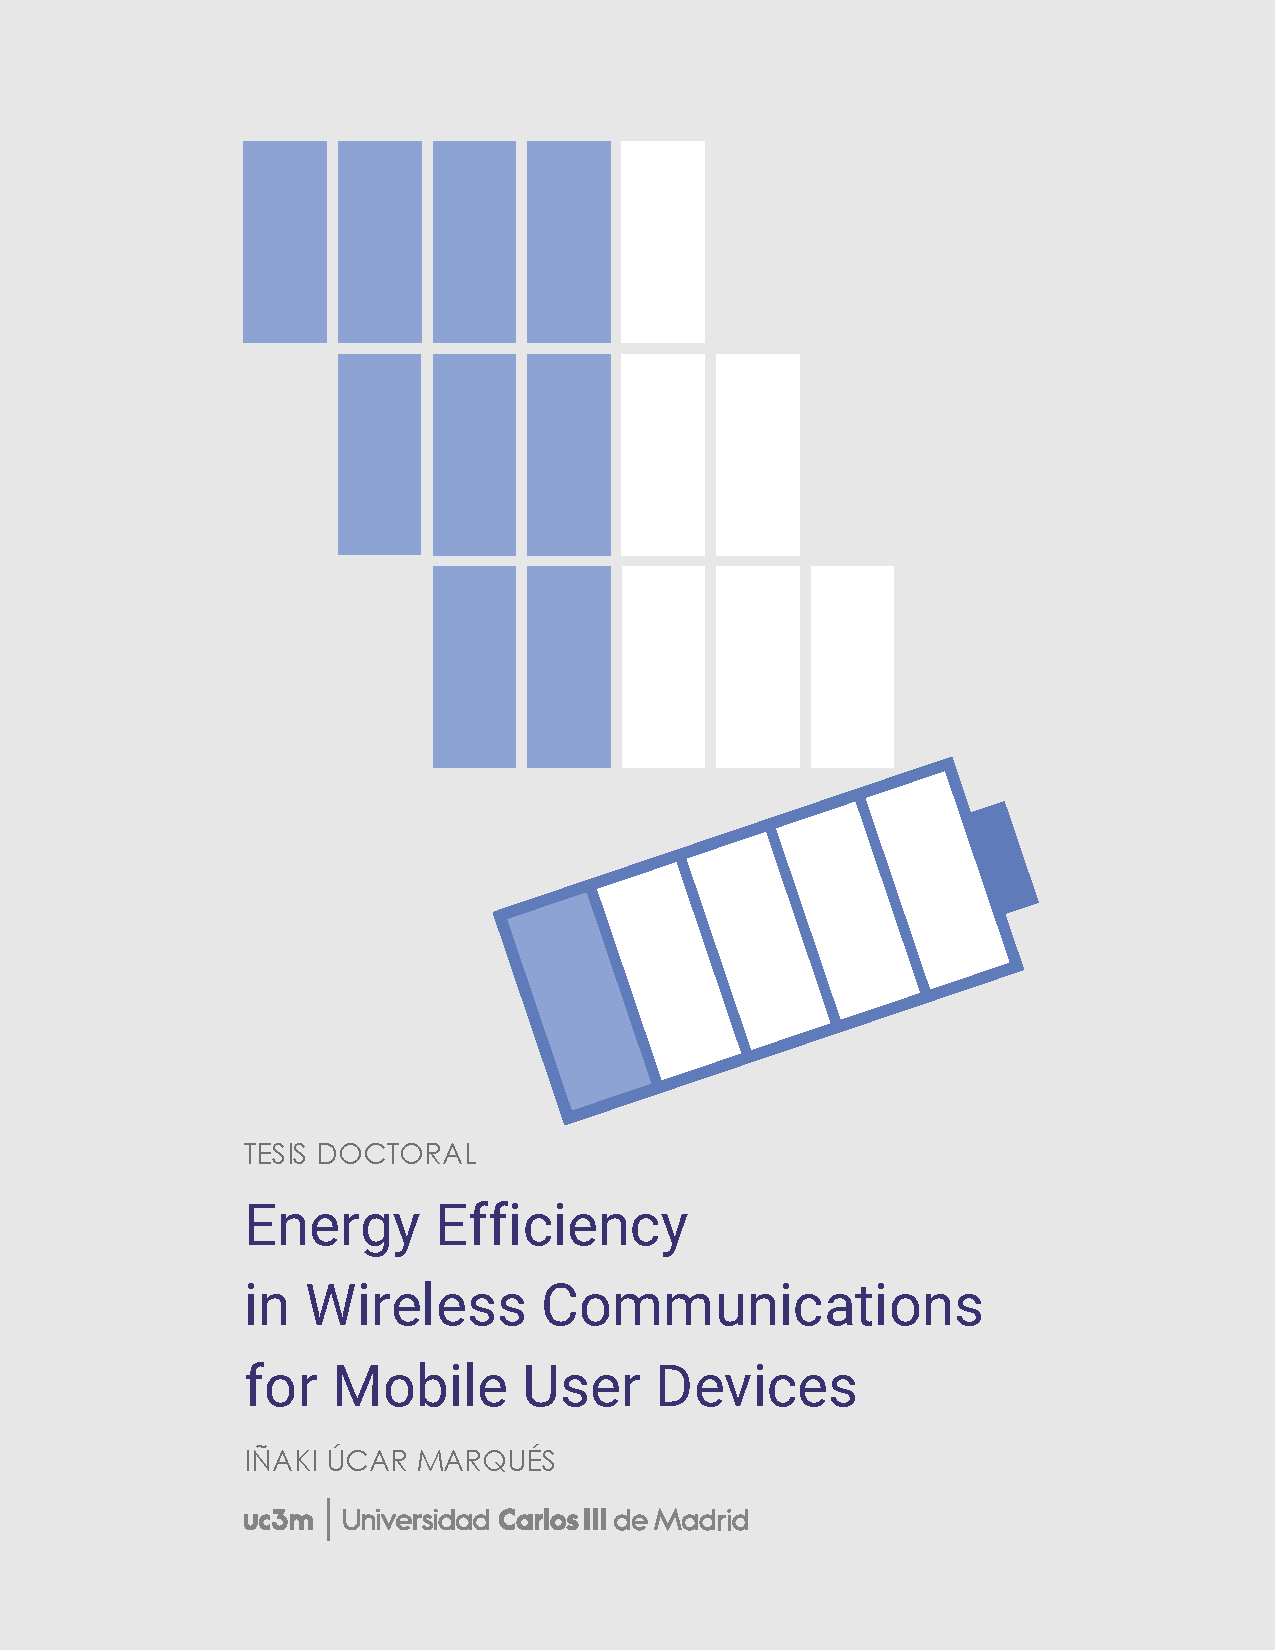
\includepdf{img/cover-front.pdf}
  \frontmatter\pagenumbering{roman}
  \begin{fullwidth}\flushright
  \thispagestyle{empty}\setlength{\parindent}{0pt}
  {
\includegraphics[width=\textwidth]{img/uc3m.eps}\par}
  
  \begingroup\color{uc3m}
    \vspace{2in}{\fontsize{14}{20}\selectfont\textsf{\smallcaps{Tesis doctoral}}\par}
    \vspace{0.2in}{\fontsize{22}{34}\selectfont\@title\par}
  \endgroup
  
  \vspace{0.2in}{\fontsize{14}{26}\selectfont\textsf{\smallcaps{Autor: \@author}}\par}
  {\fontsize{14}{20}\selectfont\textsf{\smallcaps{Director: Dr. Arturo Azcorra Saloña}}\par}
  
  \vfill{\fontsize{14}{20}\selectfont
    \textit{Doctorado en Ingeniería Telemática $\cdot$ Leganés, mayo de 2018}
  \par}
  \end{fullwidth}
  
  \newpage
  
  % copyright page
  \begingroup
  ~\vfill
  \thispagestyle{empty}\setlength{\parindent}{0pt}
  \setlength{\parskip}{\baselineskip}
  Copyright \copyright\ \the\year\ \thanklessauthor
  
  \par\smallcaps{Published by \thanklesspublisher}
  
  \begin{fullwidth}
    \par Licensed under the Creative Commons License version 3.0 under the terms of Attribution, Non-Commercial and No-Derivatives (the ``License''); you may not use this file except in compliance with the License. You may obtain a copy of the License at \url{http://creativecommons.org/licenses/by-nc-nd/3.0}. Unless required by applicable law or agreed to in writing, software distributed under the License is distributed on an \smallcaps{``AS IS'' BASIS, WITHOUT WARRANTIES OR CONDITIONS OF ANY KIND}, either express or implied. See the License for the specific language governing permissions and limitations under the License.\index{license}
  \end{fullwidth}
  
  \par\textit{First printing, May 2018}
  \endgroup
  
  \newpage
  
  \begin{fullwidth}\flushright
  \thispagestyle{empty}\setlength{\parindent}{0pt}
  {
\includegraphics[width=\textwidth]{img/uc3m.eps}\par}
  
  \begingroup\color{uc3m}
    \vspace{2in}{\fontsize{14}{20}\selectfont\textsf{\smallcaps{Tesis doctoral}}\par}
    \vspace{0.2in}{\fontsize{14}{20}\selectfont\@title\par}
  \endgroup
  
  \vspace{0.2in}{Autor: \@author\par}
  {Director: Dr. Arturo Azcorra Saloña\par}
  
  \vfill\extrarowsep=5mm\begin{tabu}{X[3]X[1]}
    Tribunal Calificador: & Firma: \\
    \toprule
    Presidente: & \\
    Vocal: & \\
    Secretario: & \\
    \bottomrule
    Calificación:
  \end{tabu}
  
  \vfill{\textit{Leganés, a \qquad de \qquad\qquad de 2018}\par}
  \end{fullwidth}
  
  \cleardoublepage
  
  \begingroup
  ~\vfill
  \thispagestyle{empty}
  \begin{fullwidth}
  \begin{doublespace}
  \begin{flushright}
    {\fontsize{14}{18}\selectfont
    ``Good scientific writing is not a matter of life and death; \\\textbf{it is much more serious than that}.''}
    
    \bigskip---Robert A. Day, in \emph{How to Write and Publish a Scientific Paper}.
  \end{flushright}
  \end{doublespace}
  \end{fullwidth}
  \vfill\vfill
  \endgroup
}
\makeatother

% abstract(s)
\newenvironment{abstract}{
  \restorefullwidth
  \let\cleardoublepage\clearpage
  \begin{parcolumns}[colwidths={1=.441\linewidth},rulebetween]{2}
  \chapter*{Abstract\hskip 0pt plus .466 fill Resumen\hfill}
}{\end{parcolumns}}

% list of figures and tables
\newcommand{\listoffiguresandtables}{
  \begingroup
  \makeatletter
  %\listoffigures
  \chapter*{List of Figures and Tables}
  \addcontentsline{toc}{chapter}{List of Figures and Tables}
  \section*{List of Figures}
  \@starttoc{lof}
  \let\clearpage\relax
  %\listoftables
  \section*{List of Tables}
  \@starttoc{lot}
  \makeatother
  \endgroup
}

% equation numbers as marginnotes
\makeatletter
\let\orig@maketag@@@\maketag@@@
\renewcommand{\eqref}[1]{\textup{\let\maketag@@@\orig@maketag@@@\tagform@{\ref{#1}}}}
\def\maketag@@@#1{\hbox{\rlap{\kern\marginparsep\m@th\normalfont#1}\kern1sp}}
\makeatother

% algorithm
\makeatletter
\newcommand{\StatexIndent}[1][3]{%
  \setlength\@tempdima{\algorithmicindent}%
  \Statex\hskip\dimexpr#1\@tempdima\relax}

\newcommand*{\algrule}[1][\algorithmicindent]{\makebox[#1][l]{\hspace*{.5em}\vrule height .75\baselineskip depth .25\baselineskip}}%

\newcount\ALG@printindent@tempcnta
\def\ALG@printindent{%
  \ifnum \theALG@nested>0% is there anything to print
    \ifx\ALG@text\ALG@x@notext% is this an end group without any text?
      % do nothing
      \addvspace{-3pt}% FUDGE for cases where no text is shown, to make the rules line up
    \else
      \unskip
      % draw a rule for each indent level
      \ALG@printindent@tempcnta=1
      \loop
          \algrule[\csname ALG@ind@\the\ALG@printindent@tempcnta\endcsname]%
          \advance \ALG@printindent@tempcnta 1
      \ifnum \ALG@printindent@tempcnta<\numexpr\theALG@nested+1\relax% can't do <=, so add one to RHS and use < instead
      \repeat
    \fi
  \fi
}%
% the following line injects our new indent handling code in place of the default spacing
\patchcmd{\ALG@doentity}{\noindent\hskip\ALG@tlm}{\ALG@printindent}{}{\errmessage{failed to patch}}
\makeatother

\newcommand{\PSalgorithm}[3]{
\begin{figure}[#1]
\begin{algorithm}[H]
 \setstretch{1}
 \caption{#3}
 \label{#2}
 \begin{algorithmic}[1]
 \State ... \Comment {Initialisation}
 \State \textbf{global} $C \gets$ \textbf{true} \Comment {Contention flag}
 \Loop \Comment {Main loop}
  \State ...
  \While {bytes remaining} \Comment {Receiving loop}
    \State \Call {Read}{}
    \If {$R_A = $ BSSID OR ($T_A = $ BSSID AND
    \StatexIndent[2] \quad $R_A$ is other unicast MAC) }
      \State \Call {Set\_Sleep}{$\Delta t_\mathrm{DATA}, \Delta t_\mathrm{NAV}$}
    \EndIf
  \EndWhile
  \State \Call {Check\_FCS}{} \Comment {Frame received}
  \If {is Beacon AND $\Delta t_\mathrm{NAV}>0$} \Comment {CFP starts}
    \State $C \gets$ \textbf{false}
  \ElsIf {is CF\_End} \Comment {CFP ends}
    \State $C \gets$ \textbf{true}
  \EndIf
  \State ...
 \EndLoop
 \Procedure {Set\_Sleep}{$\Delta t_\mathrm{DATA}, \Delta t_\mathrm{NAV}$}
  \State $\Delta t_\mathrm{sleep} \gets \Delta t_\mathrm{DATA} + \Delta t_\mathrm{SIFS}$
  \If {$C$ AND is not CTS AND $\Delta t_\mathrm{NAV} \le 32 767$}
    \State $\Delta t_\mathrm{sleep} \gets \Delta t_\mathrm{sleep} + \Delta t_\mathrm{NAV}$
  \EndIf
  \If {$\Delta t_\mathrm{sleep} \ge \Delta t_\mathrm{sleep,min}$}
    \State \Call{Sleep}{$\Delta t_\mathrm{sleep}$}
    \State \Call{Wait}{$\Delta t_\mathrm{DIFS} - \Delta t_\mathrm{SIFS}$}
    \State \textbf{go to} Main loop
  \EndIf
  \State \textbf{go to} Receiving loop
 \EndProcedure
 \end{algorithmic}
\end{algorithm}
\end{figure}
}

\usepackage{amsthm}
\newtheorem{theorem}{Theorem}[chapter]
\newtheorem{lemma}{Lemma}[chapter]
\theoremstyle{definition}
\newtheorem{definition}{Definition}[chapter]
\newtheorem{corollary}{Corollary}[chapter]
\newtheorem{proposition}{Proposition}[chapter]
\theoremstyle{definition}
\newtheorem{example}{Example}[chapter]
\theoremstyle{definition}
\newtheorem{exercise}{Exercise}[chapter]
\theoremstyle{remark}
\newtheorem*{remark}{Remark}
\newtheorem*{solution}{Solution}
\begin{document}

\maketitle

\begin{abstract}
\colchunk{

\newthought{Mobile user devices'} market has experienced an 
exponential growth worldwide over the last decade, and wireless communications
are the main driver for the next generation of 5G networks. The ubiquity of
battery-powered connected devices makes energy efficiency a major research
issue.

While most studies assumed that network interfaces dominate the energy
consumption of wireless communications, a recent work unveils that the frame
processing carried out by the device could drain as much energy as the
interface itself for many devices. This discovery poses doubts on prior energy
models for wireless communications and forces us to reconsider existing
energy-saving schemes.

\quad

\newthought{From this standpoint}, this thesis is devoted to the
study of the energy efficiency of mobile user devices at multiple layers. To
that end, we assemble a comprehensive energy measurement framework, and a
robust methodology, to be able to characterise a wide range of mobile devices,
as well as individual parts of such devices.

Building on this, we first delve into the energy consumption of frame
processing within the devices' protocol stack. Our results identify the CPU as
the leading cause of this energy consumption. Moreover, we discover that the
characterisation of the energy toll ascribed to the device is much more
complex than the previous work showed. Devices with complex CPUs (several
frequencies and sleep states) require novel methodologies and models to
successfully characterise their consumption.

We then turn our attention to lower levels of the communication stack by
investigating the behaviour of idle WiFi interfaces. Due to the design of the
802.11 protocol, together with the growing trend of network densification,
WiFi devices spend a long time receiving frames addressed to other devices
when they might be dormant. In order to mitigate this issue, we study the
timing constraints of a commercial WiFi card, which is developed into a
standard-compliant algorithm that saves energy during such transmissions.

At a higher level, rate adaptation and power control techniques adapt data
rate and output power to the channel conditions. However, these have been
typically studied with other metrics rather than energy efficiency in mind
(i.e., performance figures such as throughput and capacity). In fact, our
analyses and simulations unveil an inherent trade-off between throughput and
energy efficiency maximisation in 802.11. We show that rate adaptation and
power control techniques may incur inefficiencies at mode transitions, and we
provide energy-aware heuristics to make such decisions following a
conservative approach.

Finally, our research experience on simulation methods pointed us
towards the need for new simulation tools commited to the middle-way approach:
less specificity than complex network simulators in exchange for easier and
faster prototyping. As a result, we developed a process-oriented and
trajectory-based discrete-event simulation package for the R language, which
is designed as a easy-to-use yet powerful framework with automatic monitoring
capabilities. The use of this simulator in networking is demonstrated through
the energy modelling of an Internet-of-Things scenario with thousands of 
metering devices in just a few lines of code.

}\colchunk{

\newthought{El mercado} de los dispositivos de usuario móviles 
ha experimentado un crecimiento exponencial a nivel mundial en la última
década, y las comunicaciones inalámbricas son el principal motor de la
siguiente generación de redes 5G. La ubicuidad de estos dispositivos
alimentados por baterías hace de la eficiencia energética un importante tema
de investigación.

Mientras muchos estudios asumían que la interfaz de red domina el consumo
energético de las comunicaciones inalámbricas, un trabajo reciente revela que
el procesado de tramas que se lleva a cabo en el dispositivo podría gastar
tanta energía como la propia interfaz para muchos dispositivos. Este
descubrimiento plantea dudas sobre los anteriores modelos energéticos para
comunicaciones inalámbricas y nos obliga a reconsiderar los esquemas de ahorro
energético existentes.

\quad

\newthought{Desde este punto de vista}, esta tesis está
dedicada al estudio de la eficiencia energética de dispositivos de usuario
móviles en múltiples capas. Para ello, se construye un completo sistema de
medida de energía, y una metodología robusta, capaz de caracterizar un amplio
rango de dispositivos móviles, así como partes individuales de tales
dispositivos.

A partir de esto, en primer lugar se profundiza en el consumo energético del
procesamiento de tramas en la pila de protocolos de los dispositivos. Nuestros
resultados identifican a la CPU como principal causa de tal consumo. Además,
se descubre que la caracterización de la cuota energética adscrita al
dispositivo es mucho más compleja que lo mostrado por el trabajo anterior. Los
dispositivos con CPU complejas (múltiples frecuencias y modos de apagado)
requieren nuevas metodologías y modelos para caracterizar su consumo de manera
existosa.

En este punto, volvemos nuestra atención hacia niveles más bajos de la pila de
comunicaciones para investigar el comportamiento de las interfaces WiFi en
estado inactivo. Debido al diseño del protocolo 802.11, junto con la tendencia
creciente hacia la densificación de las redes, los dispositivos WiFi pasan
mucho tiempo recibiendo tramas destinadas a otros dispositivos cuando podrían
estar apagados. Para mitigar este problema, se estudian las limitaciones
temporales de una tarjeta WiFi comercial, lo que posteriormente se utiliza
para desarrollar un algoritmo conforme con el estándar que es capaz de ahorrar
energía durante dichas transmisiones.

A un nivel más alto, las técnicas de adaptación de tasa y control de potencia
adaptan la tasa de datos y la potencia de salida a las condiciones del canal.
No obstante, estas técnicas han sido típicamente estudiadas con otras métricas
en mente (i.e., figuras de rendimiento como la tasa total y la capacidad).
De hecho, nuestros análisis y simulaciones desvelan un conflicto entre la
maximización de la tasa total y la eficiencia energética en 802.11. Se muestra
que las técnicas de adaptación de tasa y control de potencia pueden incurrir
en ineficiencias en los cambios de modo, y se proporcionan heurísticos para
tomar tales decisiones de un modo conservador y eficiente energéticamente.

Finalmente, nuestra experiencia investigadora en métodos de
simulación nos hizo conscientes de la necesidad de nuevas herramientas de
simulación comprometidas con un enfoque intermedio: menos especificidad que
los complejos simuladores de redes a cambio de facilidad y rapidez en el
prototipado. Como resultado, se desarrolló un paquete de simulación por
eventos discretos para el lenguaje R orientado a procesos y basado en
trayectorias, el cual está diseñado como una herramienta fácil de utilizar a
la par que potente con capacidad de monitorización automática integrada. El
uso de este simulador en redes se demuestra mediante el modelado en energía
de un escenario de la Internet de las Cosas con miles de dispositivos de
medida en tan solo unas pocas líneas de código.

}
\end{abstract}


{
\setcounter{tocdepth}{1}
\tableofcontents
}

\listoffigures

\hypertarget{preface}{%
\chapter*{Preface}\label{preface}}
\addcontentsline{toc}{chapter}{Preface}

\newthought{Perhaps the reader} reaches these words expecting a long
diatribe about climate change and greenhouse emissions, about how we are
wrecking our ecosystems. But I am \emph{not} doing that. I am bored of
it. I do not do it in the same way as a dissertation on astrophysics
does not see fit to mention the fact that the Earth orbits the Sun: it
should be obvious for everybody at this point. Instead, I will be
appealing to a more selfish reason.

\newthought{The preface} of Matthew Gast's \emph{802.11 Wireless
Networks} summarises the tremendous success of wireless networks with
just a couple of short bold statements:

\begin{quote}
\emph{People move. Networks don't.}
\end{quote}

And although some researchers may be in a position to start to question
the latter, I think that we all can agree on the first one. There is one
small quibble though: \emph{people move\ldots{} for as long as their
mobile devices allow them}. In fact, who has not experienced desperately
looking for a socket in a cafeteria, a conference room, a metro station,
a bus, an airport\ldots{} because the phone is \emph{dead}. As quarks
inside a hadron\footnote{I know, I couldn't help it.}, wireless devices
have given us the freedom of mobility, but also the slavery of the
battery.

To sum up, we not only want \emph{mobility}, but also
\emph{long-lasting} mobility. But the consumption of the wireless link
is insignificant compared to the consumption of the screen, one might
say. And it is true. However, if we for instance think of a smartphone,
it is also true that it is in our pocket for most of the day, unused but
still connected, managing instant notifications for multiple services.
As a result, it is not uncommon to see the data connection as a top
consumer in the phone's battery manager. So we can do better, and that
is what this thesis is about.

\newthought{I still remember} the first time I met my advisor in a Skype
interview. ``What do you like the most: experimentation, mathematical
modelling or simulation?'', it was one of the first things that he was
interested to know. I replied that I like them all, but if I
can\footnote{Because sometimes you simply do not have the resources.}
choose, I like experimental work the most. Because, for me, this is the
\emph{real} science; because, as Aristotle first reflected,
\emph{empiricism}, \emph{careful observation}, is the starting point for
\emph{episteme}. In fact, the Spanish verb for ``to see'', which is
\emph{``ver''}, shares the Indo-European root \emph{*weid-} with the
English adjective ``wise'': \emph{I see, therefore I know}.

Still, I am a very curious person who likes to explore the many
techniques available, and I think that this thesis is a faithful
reflection of such curiosity. Thanks to this, during this journey I
discovered myself as an open source enthusiast who enjoys making tools
that are useful for other people. I even managed to grow a small
community of users around one of such tools. Receiving feedback from
them is extremely fulfilling, and for that I am very grateful.

But my curiosity is not limited to the method and extends to the
research topics, as my publication record, including those prior to my
PhD, inevitably evidences. The good thing about a PhD is that you have
to focus on a specific topic; the bad thing about a PhD is that
\emph{you have to focus on a specific topic}. I have to admit that
sometimes this has been a little burden to me which I hardly managed to
overcome.

All in all, this has been a great experience. In fact, one of the best
experiences of my life: I have met many interesting people from around
the world, I have learned a lot from them and I have grown in every way
as a person. Now this stage ends and an uncertain future opens up. But I
am not afraid of it, because I am convinced that the best is yet to
come.

\begin{marginfigure}

{\centering 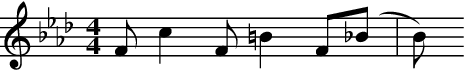
\includegraphics[width=1\linewidth]{img/tbiytc} 

}

\end{marginfigure}

\hypertarget{acknowledgements}{%
\section*{Acknowledgements}\label{acknowledgements}}

I would like to begin by thanking my advisor, Arturo Azcorra, for giving
me the opportunity of pursuing this PhD, and for being supportive and
placing his trust in me even when I was beset by the
\emph{Publish-or-Perish} difficulties. His advice and guidance have been
very valuable. I also wish to extend my thanks to UC3M's Department of
Telematics Engineering, and to the NETCOM research group in particular,
for supporting me. I have been privileged to work with and learn from
great people.

I would also like to express my gratitude and sincere appreciation to
all my co-authors, who always provide productive discussion, input and
advice, and to all those who have helped me, shared their knowledge with
me and guided my teaching experience.

My special thanks are due to Pablo Serrano, who in turn belongs to the
latter two groups, and who has been like a second advisor to me; to
Andrés García Saavedra, who is an outstanding engineer and scientist,
and whose guidance during the initial stage of my PhD was invaluable; to
Ernesto García Ares, for his help and excellent work at UC3M's Technical
Office in Electronics; to Bart Smeets, for his support, kindness and
generosity. And of course to Francesco Gringoli, for having me during a
great stay in Brescia. I was honored, and I really enjoyed a lot working
closely with him; if I have not managed to fit part of that work in this
dissertation, it is just my fault.

I am also indebted to so many others than would not fit in these pages.
All my lab mates, past and present, and especially Luca, with whom I
have shared the path since its very beginning, have contributed to a
great working environment and have become my friends. Marco brought the
seed of passion for tennis, which reached me through Fabio, and thanks
to them I found an unparalleled stress reliever. Fernando's lessons and
all my tennis mates have undoubtedly contributed to my sanity during
this years.

And still, none of this would have been possible without the intangible
contribution of a number of supportive relatives and friends. This
thesis is especially dedicated to Almudena, who indulged me despite all
the weekends and plans that were sacrificed to the contents of this
book.

\begin{quote}
\hfill ---Iñaki Úcar

\hfill Madrid, May 2018
\end{quote}

\mainmatter\pagenumbering{arabic}

\hypertarget{introduction}{%
\chapter{Introduction}\label{introduction}}

\newthought{Energy efficiency} is the ability to do more with less. When
we talk about \emph{green communications}, this means more connectivity,
more capacity and more responsiveness at a lower energy cost.
Unfortunately, these are competing goals, and all we can do in this tale
is to fight against thermodynamics to seek for the elusive
\emph{optimality}.

It is straightforward to compute the minimum energy required to move a
mass on a surface from point A to point B, as it depends on the friction
coefficient. Drawing a parallelism, we are interested in the
\emph{friction}\cite[0pt]{grover2015}\marginnote{\hypersetup{hidelinks}\color{white}\citet{grover2015}}
of communicating a \emph{bit} from point A to point B. As in the
Newtonian example, our problem depends on the \emph{substrate}, the
specific technology and implementation. But when we deal with such
complex systems as today's telecommunications networks, this estimation
remains unfeasible.

We walk blindly towards an unknown lower bound. Fortunately, the set of
possible strategies are limited and
well-known\cite[0pt]{samdanis2015green}\marginnote{\hypersetup{hidelinks}\color{white}\citet{samdanis2015green}},
and pursue a common objective, namely, that the energy consumption
should be proportional to the transmitted information. These can be
divided in three basic principles subject of active research, and their
intent can be summarised as follows:

\begin{description}
\tightlist
\item[Speed scaling,]
which tries to adapt the processing speed of network devices to the
traffic load.
\item[Powering down,]
which aims to turn network devices off during inactivity periods. This
is commonly implemented as the so-called \emph{sleep states}, and their
\emph{depth} introduces an inherent trade-off with the time required to
become active again.
\item[Rate adaptation,]
which tries to adapt the transmission rate of wireless cards according
to the channel conditions\footnote{This, as well as the \emph{speed
  scaling} principle, is based on a direct relationship between
  consumption and transmission rate, which is not always the case.}.
\end{description}

The aim of this thesis is to explore the above three strategies in the
scope of wireless communications for mobile user devices at multiple
layers, as will be introduced in the following sections: from the
operating system to the low-level operation of the wireless card.

\hypertarget{cross-factor-towards-a-new-energy-model}{%
\section{Cross-Factor: Towards a New Energy
Model}\label{cross-factor-towards-a-new-energy-model}}

We are living in an era in which consumer electronics are becoming
\emph{wireless consumer electronics}. That is, just about any known
gadget is capable of connecting to cellular, wireless Local Area
Networks (WLAN) or wireless Personal Area Networks (WPAN) nowadays. The
Internet of Things (IoT) is growing fast and wireless communications
become its main driver. Due to the densification of wireless networks
and the ubiquity of battery-powered devices, energy efficiency stands as
a major research issue.

More and more devices around us are becoming \emph{smart}, incorporating
more processing power in order to do more things, and some of them are
already comparable to a small laptop computer. As a consequence, not
only do they share hardware components, but also software: in
particular, the Linux kernel is spreading into billions of devices all
over the world, whether inside of the popular Android operating system
or other embedded systems.

Whereas a lot of research were and is devoted to obtain more
energy-efficient hardware components (e.g., wireless cards, processors,
screens), too little attention has been paid, in terms of energy, to a
core software component that enables all these devices: the operating
system and, inside it, the network stack.

\newthought{The seminal paper} by \citet{Feeney2001}\cite{Feeney2001}
gives the very first insight on energy consumption of wireless
interfaces. This work was done on a per-frame basis by accounting for
the energy drained by an 802.11 wireless card. Subsequent experimental
work followed the same approach, showing that the energy consumption of
wireless transmissions/receptions can be characterised using a simple
linear model. This fact arises from the three typical states of
operation of a wireless card: idle, transmitting and receiving.

The model, commonly expressed in terms of power, has a fixed part
\(\rho_{id}\), device-dependent, attributable to the idle state, and it
grows linearly with the airtime percentage \(\tau\) (i.e., the fraction
of time in which the card is transmitting or receiving).

However, more recently, the novel work by
\citet{Serrano2014}\cite{Serrano2014} performed extensive per-frame
measurements for seven devices of different types (smartphones, tablets,
embedded devices and wireless routers), and unveiled that actually there
is a non-negligible per-frame processing toll ascribed to the frame
crossing the network stack. This component emerges as a new offset
proportional to the frame generation rate, and it is not explained by
the \emph{classical} model.

\pagebreak

The currently accepted energy model is a multilinear model articulated
into three main parts:
%
\begin{equation}
 \overline{P}(\tau_i, \lambda_i) = \underbrace{\rho_\mathrm{id} + \sum_{i\in\mathrm{\{tx,rx\}}} \rho_i \tau_i}_{\text{classical model}} + \sum_{i\in\mathrm{\{g,r\}}} \gamma_{\mathrm{x}i} \lambda_i
 \label{eq:new-energy-model}
\end{equation}
%
where the first two addends correspond to the classical model and the
third is the contribution described in \citet{Serrano2014}. This model
can be subdivided into five components:

\begin{itemize}
\tightlist
\item
  A platform-specific baseline power consumption that accounts for the
  energy consumed just by the fact of being powered on, but with no
  network activity. This component is commonly referred to as \emph{idle
  consumption}, \(\rho_\mathrm{id}\).
\item
  A component that accounts for the energy consumed in transmission,
  which grows linearly with the airtime percentage
  \(\tau_\mathrm{tx}\)\marginnote{$\overline{P_\mathrm{tx}}(\tau_\mathrm{tx}) = \rho_\mathrm{tx} \tau_\mathrm{tx}$}.
  The slope \(\rho_\mathrm{tx}\) depends linearly on the radio
  transmission parameters MCS and TXP.
\item
  A component that accounts for the energy consumed in reception, which
  grows linearly with the airtime percentage
  \(\tau_\mathrm{rx}\)\marginnote{$\overline{P_\mathrm{rx}}(\tau_\mathrm{rx}) = \rho_\mathrm{rx} \tau_\mathrm{rx}$}.
  The slope \(\rho_\mathrm{rx}\) depends linearly on the radio
  transmission parameter MCS.
\item
  A new component, called \emph{generation cross-factor} or
  \(\gamma_{\mathrm{xg}}\), that accounts for a per-frame energy
  processing toll in transmission, which grows linearly with the traffic
  rate \(\lambda_\mathrm{g}\)
  generated\marginnote{$\overline{P_\mathrm{xg}}(\lambda_\mathrm{g}) = \gamma_\mathrm{xg} \lambda_\mathrm{g}$}.
  The slope \(\gamma_\mathrm{xg}\) depends on the computing
  characteristics of the device.
\item
  A new component, called \emph{reception cross-factor} or
  \(\gamma_{\mathrm{xr}}\), that accounts for a per-frame energy
  processing toll in reception, which grows linearly with the traffic
  rate \(\lambda_\mathrm{r}\)
  received\marginnote{$\overline{P_\mathrm{xr}}(\lambda_\mathrm{r}) = \gamma_\mathrm{xr} \lambda_\mathrm{r}$}.
  Likewise, the slope \(\gamma_\mathrm{xr}\) depends on the computing
  characteristics of the device.
\end{itemize}

Therefore, the average power consumed \(\overline{P}\) is a function of
five device-dependent parameters (\(\rho_i, \gamma_{\mathrm{x}i}\)) and
four traffic-dependent ones (\(\tau_i, \lambda_i\)).

The results obtained with this new multilinear model showed that the
so-called cross-factor accounts for 50\% to 97\% of the per-frame energy
consumption. Additional findings showed that it is independent of the
CPU load on some devices and \emph{almost} independent of the frame
size.

Therefore, this inspired us to deepen into the roots of the
cross-factor, to deseed its components and analyse its causes. To this
aim, it is of paramount importance the conception of a comprehensive,
high-accuracy and high-precision measurement framework that enables us
to measure the consumption of a wide range of mobile devices.

\hypertarget{micro-sleep-opportunities-in-802.11}{%
\section{Micro-Sleep Opportunities in
802.11}\label{micro-sleep-opportunities-in-802.11}}

IEEE 802.11 is an extremely common technology for broadband Internet
access. Energy efficiency stands as a major issue due to the intrinsic
CSMA mechanism, which forces the network card to stay active performing
\emph{idle listening}, while most of the 802.11-capable terminals run on
batteries.

The 802.11 standard developers are fully aware of the energy issues that
WiFi poses on battery-powered devices and have designed mechanisms to
reduce energy consumption. One of such mechanisms is the Power Save (PS)
mode, which is widely deployed among commercial wireless cards, although
unevenly supported in software drivers. With this mechanism, a station
(STA) may enter a doze state during long periods of time, subject to
prior notification, if it has nothing to transmit. Meanwhile, packets
addressed to this dozing STA are buffered and signalled in the Traffic
Indication Map (TIM) attached to each beacon frame.

The PS mechanism dramatically reduces the power consumption of a
wireless card. However, the counterpart is that, since the card is put
to sleep for hundreds of milliseconds, the user experiences a serious
performance degradation because of the delays incurred. The automatic
power save delivery (APSD) introduced by the 11e amendment
(\citet{Perez-Costa2010}\cite{Perez-Costa2010} give a nice overview) is
based on this mechanism, and aims to improve the downlink delivery by
taking advantage of QoS mechanisms, but has not been widely adopted.

More recently, the 11ac amendment improves the PS capabilities with the
VHT TXOP (Very High Throughput, Transmission Opportunity) PS mechanism.
Basically, an 11ac STA can doze during other STAs' TXOPs. This
capability is announced within the new VHT framing format, so that the
AP knows that it cannot send traffic to those STAs until the TXOP's
natural end, even if it is interrupted earlier. Still, the potential
dozing is in the range of milliseconds and may lead to channel underuse
if these TXOPs are not fully exploited.

Considering shorter timescales, packet overhearing (i.e., listening to
the wireless while there is an ongoing transmission addressed to other
station) has been identified as a potential source of energy
waste\cite[0pt]{basu2004}\marginnote{\hypersetup{hidelinks}\color{white}\citet{basu2004}}.
Despite this, our measurements found no trace of mechanisms in
commercial wireless card to lessen its impact.

Taking advantage on the energy measurement framework built for this
thesis, we further investigate the timing capabilities for transitioning
between operational states of a commercial off-the-shelf (COTS) wireless
card. Based on this, we propose \(\mu\)Nap, a practical algorithm to
leverage micro-sleep opportunities in 802.11 WLANs.

\hypertarget{rate-adaptation-and-power-control-in-802.11}{%
\section{Rate Adaptation and Power Control in
802.11}\label{rate-adaptation-and-power-control-in-802.11}}

At the beginning of this introduction, we have identified rate
adaptation as one of the three basic strategies that can be applied to
achieve proportionality between energy consumption and traffic load.
Nevertheless, energy efficiency has not been the main driver for
research in the fields of rate adaptation and power control in 802.11.

Rate adaptation (RA) algorithms are responsible for selecting the most
appropriate modulation and coding scheme (MCS) to use given an
estimation of the link conditions, being the frame losses one of the
main indicators of such conditions. In general, the challenge lies in
distinguishing between those losses due to collisions and those due to
poor radio conditions, because they should trigger different reactions.
In addition, the performance figure to optimise is commonly the
throughput or a related one such as, e.g., the time required to deliver
a frame.

On the other hand, network densification is becoming a common tool to
provide better coverage and capacity. However, densification brings new
problems, especially for 802.11, given the limited amount of orthogonal
channels available, which leads to performance and reliability issues
due to radio frequency interference. In consequence, some RA schemes
also incorporate transmission power control (TPC), which tries to
minimise the transmission power (TXP) with the purpose of reducing
interference between nearby networks. As in the case of ``vanilla'' RA,
the main performance figure to optimise is also the throughput.

It is generally assumed that optimality in terms of throughput also
implies optimality in terms of energy efficiency. However, some previous
work\cite[0pt]{Li2012,khan2013}\marginnote{\hypersetup{hidelinks}\color{white}\citet{Li2012,khan2013}}
has shown that throughput maximisation does not result in energy
efficiency maximisation, at least for 802.11n. However, we still lack a
proper understanding of the causes behind this ``non-duality'', as it
may be caused by the specific design of the algorithms studied, an extra
consumption caused by the complexity of MIMO techniques, or any other
reason.

This thesis revisits RA-TPC in 802.11 within the context of energy
efficiency. We first conduct an analytical study, and then we evaluate
the performance, in terms of energy, of several state-of-the-art RA-TPC
algorithms by simulation. Our results unveil that the trade-off shown by
previous studies is in turn inherent to 802.11 operation. Particularly,
we show that the link quality conditions which trigger mode transitions
(changes of MCS/TXP) may be source of inefficiencies. Nonetheless, our
analyses provide some heuristics that can be used along the energy
parameters of the wireless card to mitigate such inefficiencies.

\hypertarget{applied-simulation-modelling-for-energy-efficiency}{%
\section{Applied Simulation Modelling for Energy
Efficiency}\label{applied-simulation-modelling-for-energy-efficiency}}

Simulation frameworks are undoubtedly one of the most important tools
for the analysis and design of communication networks and protocols.
Their applications are numerous, including the performance evaluation of
existing or novel proposals, dimensioning of resources and capacity
planning, or the validation of theoretical analyses.

Simulation frameworks make a number of simplifying assumptions to reduce
complexity so the development of the scenario is easier and numerical
figures are obtained faster. This ``complexity'' axis goes from very
specialised, large simulation tools such as NS-3, OMNeT++, OPNET, to
\emph{ad-hoc} simulation tools, consisting on hundreds of lines of code,
typically used to validate a very specific part of the network or a
given mathematical analysis. The latter are often developed over
general-purpose languages such as C/C++ or Python, over numerical
frameworks such as Matlab, or over some framework for discrete-event
simulation (DES).

On the one hand, the complexity of specialised tools (as their cost, if
applicable) preclude their use for short-to-medium research projects, as
the learning curve is typically steep plus they are difficult to extend,
which is mandatory to test a novel functionality. On the other hand, the
development of ad-hoc tools also require some investment of time and
resources, lack a proper validation of their functionality, and,
furthermore, there is no code maintenance once the project is finished,
for the few cases in which the code is made publicly available.

Last but not least, the monitoring of variables of interest typically
stands out as a first-order problem. Most simulators require a specific
effort in this regard, so that the modeller has to ponder which
parameters must be monitored, and where and how this should be done.
Therefore, the design of the scenario is intrinsically linked to data
collection.

The research experience gained over the course of this thesis have made
us aware of the need for new simulation tools committed to the
middle-way approach: less specificity and complexity in exchange for
faster prototyping, while supporting efficient simulation at a low
implementation cost. As a result, we developed \texttt{simmer}, a
process-oriented and trajectory-based DES package for R, which is
designed to be an easy-to-use yet powerful framework. Its most
noteworthy characteristic is the automatic monitoring capability, which
allows the user to focus on the system model. The use of this simulator
in networking is demonstrated through the energy modelling of a
5G-inspired scenario.

\hypertarget{thesis-overview}{%
\section{Thesis Overview}\label{thesis-overview}}

The remainder of this thesis is organised as follows. Chapter
\ref{ch:02} presents the relevant literature related to the topics
introduced in this chapter. Then, the dissertation is divided into three
thematic parts: \emph{experimentation}, \emph{mathematical modelling}
and \emph{simulation}. Chapter \ref{ch:03} presents a comprehensive
energy measurement framework, which has been a fundamental pillar of
this thesis. Building on this, Chapter \ref{ch:04} delves into the roots
of the cross-factor by exploring the energy consumption of the Linux
network stack. Chapter \ref{ch:05} completes the experimental part with
a study of the timing constraints of a COTS wireless card, which is
developed into a standard-compliant algorithm to leverage micro-sleep
opportunities in 802.11 WLANs. Chapter \ref{ch:06} presents a joint
goodput-energy model that unveils an inherent trade-off between
througput and energy efficiency maximisation in 802.11 when RA-TPC
techniques are applied. Chapter \ref{ch:07} further extends the latter
work by simulating and comparing the performance of several
representative RA-TPC algorithms. Closing the simulation part, Chapter
\ref{ch:08} presents our novel DES framework, and showcases its
versatility by analising the energy consumption of an Internet-of-Things
scenario with thousands of metering devices. Finally, Chapter
\ref{ch:09} contains the thesis conclusions and future lines of work.

This thesis covers the following contributions:\vspace{-1mm}

\par

\tolerance=500\relax

\begin{itemize}
\tightlist
\item
  \marginnote{Chapter \ref{ch:03}}\bibentry{contrib-03}.\vspace{8pt}
\item
  \marginnote{Chapter \ref{ch:04}}\bibentry{contrib-04a}.
\item
  \bibentry{contrib-04b}.\vspace{8pt}
\item
  \marginnote{Chapter \ref{ch:05}}\bibentry{contrib-05a}.
\item
  \bibentry{contrib-05b}.\vspace{8pt}
\item
  \marginnote{Chapter \ref{ch:06}}\bibentry{contrib-06}.\vspace{8pt}
\item
  \marginnote{Chapter \ref{ch:07}}\bibentry{contrib-07}.\vspace{8pt}
\item
  \marginnote{Chapter \ref{ch:08}}\bibentry{contrib-08a}.
\item
  \bibentry{contrib-08b}.
\end{itemize}

\par

Therefore, there is an overlap between this dissertation and the
publications listed above. Additionally, the following contributions are
not part of this thesis:

\begin{itemize}
\tightlist
\item
  \bibentry{flex5gware}.
\item
  \bibentry{5gnorma}.
\item
  \bibentry{11aa}.
\end{itemize}

\hypertarget{ch:02}{%
\chapter{Related Work}\label{ch:02}}

\newthought{In recent years}, we have witnessed an increased attention
towards ``green operation'' of networks, which is required to support a
sustainable growth of the communication infrastructures. For the case of
wireless communications, there is the added motivation of a limited
energy supply (i.e., batteries) in user mobile devices, which has
triggered a relatively large amount of work on energy
efficiency\cite[0pt]{survey}\marginnote{\hypersetup{hidelinks}\color{white}\citet{survey}}.

\hypertarget{energy-profiling-for-wireless-communications}{%
\section{Energy Profiling for Wireless
Communications}\label{energy-profiling-for-wireless-communications}}

Energy profiling is the most fundamental work on green communications.
In a similar way as \emph{software profiling} measures the duration of
function calls, \emph{energy profiling} measures the energy consumed by
each software or hardware \emph{function}, in the broad sense of the
word.

There are two energy measurement
techniques\cite[0pt]{tarkoma2014smartphone}\marginnote{\hypersetup{hidelinks}\color{white}\citet{tarkoma2014smartphone}}:
software- and hardware-assisted measurements. The former uses the
built-in battery interface integrated in many modern devices (e.g.,
smartphones, tablets), which provides readings of the dicharge curve.
Apart from the evident feedback loop problem\footnote{Namely, that the
  software used to collect such readings is in fact producing an energy
  overhead.}, this method lacks granularity and precision, and therefore
it is not suited for fine-grained energy profiling. Despite this, it has
been used in a number of papers, such as \citet{Nurminen2008},
\citet{xiao2008}, \citet{Balasubramanian2009} and \citet{kalic2012},
some of them based on \citet{creus2007optimizing}. \citet{dong2011self},
\citet{jung2012devscope} and \citet{xu2013v} try to overcome this
limitations by developing an online power model on top of the battery
monitoring unit.

Instead, in hardware-assisted measurements, the battery is bypassed to
directly measure the current and voltage\footnote{User mobile devices
  use DC power. Therefore, the voltage signal is usually ignored and
  assumed to be constant, which may not be the best approach for
  fine-grained measurements.} signals. The current signal is converted
to voltage with a small high-precision resistor, and then sampled with a
variety of instruments (digital multimeters, oscilloscopes, data
acquisition devices\ldots{}). Thus, the granularity and precision is
limited by the specific setup and instrumentation selected.

\pagebreak

Typically, energy profiling studies in wireless communications provide a
measurement setup that is expressly designed for the electrical
specifications of the device under test. For instance,
\citet{Feeney2001} and \citet{Jean-pierreEbert} use a cardbus extender
and an oscilloscope to measure wireless interfaces. \citet{Carroll2010},
\citet{Rice2010}, \citet{Wang2010} perform energy measurements on
smartphones using a data acquisition (DAQ) card, while \citet{gupta2007}
used a power meter.

More recent studies (e.g., \citet{zhang2010accurate},
\citet{pathak2011fine}, \citet{manweiler2011avoiding},
\citet{jung2012devscope}, \citet{oliner2012collaborative},
\citet{xu2013v}, \citet{kim2013runtime}, \citet{zhang2013towards})
started using the Monsoon\footnote{\url{https://www.msoon.com/}} Power
Monitor, a product specifically designed to test smartphones which has
become very popular. There have also been initiatives to design
open-source energy measurement and control systems such as
Energino\footnote{\url{http://www.energino-project.org/}}
\citep{riggio2012energino, gomez2012energino}.

\hypertarget{energy-consumption-of-network-stacks}{%
\section{Energy Consumption of Network
Stacks}\label{energy-consumption-of-network-stacks}}

The \emph{classical} energy model for wireless interfaces was first
established by \citet{Feeney2001}, and further confirmed by
\citet{Jean-pierreEbert} and \citet{Shih2002}. Since then, it has been
assumed that the network card dominates the consumption of wireless
communications of mobile user devices.

This model has been widely used (implicitly or explicitly) in tens of
papers to justify energy savings with optimisations of diverse kind: PHY
layer rate and power \citep{DajiQiao}, MAC parameters
\citep{Bruno2002, Carvalho2004, Agrawal2004, Jyh-ChengChen2008, Garcia-Saavedra2011},
backoff operation \citep{Vaidya2002, Baiamonte2006}, idle state
\citep{Zhang2012}, packet overhearing \citep{Ergen2007}, packet relying
\citep{He2010}, data compression \citep{Baek2004, Sharma2009}, etcetera.

However, the work by \citet{Serrano2014}, which provides the \emph{new}
energy model studied in the previous chapter, poses doubts on prior work
that propose energy efficiency strategies taking into account the
wireless card only. Bearing in mind these results, it is imperative to
reconsider existing schemes for energy efficiency in wireless
communications. Old schemes like packet relying \citep{He2010} and data
compression \citep{Baek2004, Sharma2009} may no longer be valid under
the new model. On the contrary, packet batching or low-level packet
generation could potentially produce real savings.

\hypertarget{micro-sleep-opportunities-in-802.11-1}{%
\section{Micro-Sleep Opportunities in
802.11}\label{micro-sleep-opportunities-in-802.11-1}}

It is well-known that the majority of nodes within any WLAN would spend
most of the time in idle state. There are two main strategies to save
energy in this idle time: the first one targets \emph{idle listening}
(the wireless channel is empty), and the second one targets \emph{packet
overhearing} (there are other nodes communicating). To support these
savings, COTS devices have two main operational states as a function of
the reference clock used: the active state and the sleep state. The more
a card stays in sleep state, the less power it consumes.

Since its conception, 802.11 has attempted to minimise idle listening
with the introduction of the PS mode, and some previous work followed
this path. For instance, \citet{Liu2008} proposed \(\mu\)PM to exploit
short idle intervals (\(<\) 100 ms) without buffering or cooperation.
\(\mu\)PM predicts the arrival time of the next frame and puts the
interface in PS mode while no arrivals are expected. This mechanism
demonstrated poor granularity (tens of ms) on existing hardware and
leads to performance degradation due to frame loss. Therefore, it is
only suitable for low-traffic scenarios.

Others propose a PS-like operation. \citet{Jang2011} described Snooze,
an access point (AP)-directed micro-sleep scheduling and antenna
configuration management method for 11n WLANs. As a consequence of its
centralised design, the granularity of the so-called micro-sleeps in
this approach is poor (few milliseconds), which poses doubts on its
performance under heavy loads.

\citet{Zhang2012} addressed the issue from a different standpoint with
their Energy-Minimizing Idle Listening (E-MiLi). E-MiLi adaptively
downclocks the card during idle periods, and reverts to full rate when
an incoming frame is detected. To achieve this purpose, they need to
change the physical layer (PHY) all the way down to enable downclocked
detection, which severely limits the potential gains. For instance, the
E-MiLi downclocking factor of 16 would yield a high power consumption in
a modern card compared to its sleep state\footnote{See Section
  \ref{characterisation-of-a-cots-device}.}.

On the other hand, all indicators show that we should expect an
exponential grow in the number of wireless devices connected. Thus,
there is a rough consensus about that \emph{densification} will become
one of the main aspects of next-generation wireless networks, which
brings us back to the problem of packet overhearing. In this way, the
recent 11ac amendment adds the ability to save energy during TXOPs, but
this mechanism is restricted to QoS traffic, and the potential sleeps
are coarse, in the range of milliseconds. Any sub-millisecond approach
must take into account the timing parameters of the hardware. In fact,
some early studies realise the importance of this issue when WiFi
technology began to take off commercially
\citep{kamerman1997, havinga2000, jung2002}.

\citet{Baiamonte2006} were the first to chase fine-grained micro-sleep
opportunities during packet overhearing. They define the
Energy-efficient Distributed Access (EDA) scheme, which uses the 802.11
virtual carrier-sensing mechanism for power-saving purposes. Basically,
a STA dozes when the Network Allocation Vector (NAV) or the backoff
counter are non-zero. Unfortunately, this work lacks an empirical
characterisation of the timing constraints needed to design a practical
mechanism. Moreover, dozing during the backoff window is not
802.11-fair: in 802.11, STAs must sense the channel every single time
slot during the contention period and, if another STA seizes the channel
first, the backoff timer must be stopped in order to receive the
incoming frame and set the NAV to the proper value. The EDA scheme
allows STAs to doze during the contention period and, therefore, breaks
the CSMA operation.

\citet{Balaji2010} revisited the problem of packet overhearing with a
scheme called Sleep during Neighbor-Addressed Frame (SNAF). With SNAF, a
wireless card checks the destination MAC address and switches to sleep
state during the payload duration if it was addressed to other host.
They assume, without any experimental validation though, an
instantaneous switch-off and that the time required to wake up is
equivalent to a Short Interframe Space (SIFS). In order to prevent the
risk resulting from errors in the frame header that would lead to an
incorrect NAV counter, the authors propose to introduce a new framing
format with a new FCS devoted to the MAC header only. This solution
lacks compatibility and introduces more overhead based on no evidence.

Building on the same idea, \citet{Prasad2014} proposed Übersleep. This
time, the authors do not consider it necessary to add any extra FCS, as
they claim (without any specific basis) that such errors are very
unlikely.

More recently, \citet{palacios2013a} and \citet{palacios2013b} modified
802.11 DCF and PCF to exploit per-packet sleeps. They also applied these
ideas to network coding \citep{palacios2015b} and to a polling-based
version of 11ac's TXOP PS mode \citep{palacios2015a}. Unfortunately, all
these papers rely on these early studies mentioned before
\citep{kamerman1997, havinga2000, jung2002}, which analysed old wireless
cards unable to perform sub-millisecond transitions between states.

\hypertarget{rate-adaptation-and-power-control-in-802.11-1}{%
\section{Rate Adaptation and Power Control in
802.11}\label{rate-adaptation-and-power-control-in-802.11-1}}

Rate adaptation and power control in 802.11 have received a vast amount
of attention from the research community (especially the former). See,
e.g., \citet{biaz2008}, \citet{h-rca} and references therein. But, as
stated before, all this research is generally focused towards
performance (i.e., throughput and capacity) maximisation.

However, as some previous work has pointed out
\citep{tradeoff, balancing}, energy efficiency and performance do not
necessarily come hand in hand, and some criterion may be required to set
a proper balance between them. Particularly, \citet{Li2012} and
\citet{khan2013} studied RA for energy efficiency in 802.11n, and showed
that MIMO RA algorithms are not energy efficient despite ensuring high
throughput. These algorithms incur inefficiencies when marginal
throughput gains are achieved at a high energy cost.

No other studies have further investigated these inefficiencies in more
detail though. The question remains, then, whether there may be
fundamental trade-offs in the application of RA-TPC techniques to
802.11.

\hypertarget{discrete-event-simulation-of-network-systems}{%
\section{Discrete-Event Simulation of Network
Systems}\label{discrete-event-simulation-of-network-systems}}

The list of network simulation tools is vast\footnote{See, e.g.,
  \url{http://people.idsia.ch/~andrea/sim/simnet.html}.}. Particularly,
OPNET\footnote{\url{http://www.opnet.com}} is one of the most complex
and widely used tools for research and education, although the
open-source alternatives, such as NS3 and OMNeT++, are growing and
becoming more prominent within the research community. As an
illustrative comparison, a quick search on Google Scholar\footnote{As of
  April 2018.} returns over 30k results for ``opnet simulation'', about
6k for ``omnet++ simulation'' and about 12k for ``ns3 simulation''. Not
surprisingly, the old version of the latter, NS2, still produces more
than 40k results. Still, the amount of research produced by the
networking community is enormous, and it is difficult to quantify how
much of that research is done using ad-hoc simulation tools.

Besides that, the list of general-purpose DES frameworks is even more
vast\footnote{See, e.g.,
  \url{https://en.wikipedia.org/wiki/List_of_discrete_event_simulation_software}.},
and most of them are unknown within the networking community because
they are generally more suited for other fields, such as operations
research. Among them, the \texttt{SimPy} Python
package\cite[0pt]{SimPy}\marginnote{\hypersetup{hidelinks}\color{white}\citet{SimPy}}
has received increased attention, and has inspired similar frameworks
for other languages, such as \texttt{SimJulia} \citep{GitHub:SimJulia}.
Nonetheless, some studies showed that SimPy may not scale for large
network simulations \citep[\citet{weingartner2009}]{bahouth2007}.

\addtocontents{toc}{\partseparator}

\hypertarget{part-experimentation}{%
\part{Experimentation}\label{part-experimentation}}

\hypertarget{ch:03}{%
\chapter{A Comprehensive Energy Measurement Framework}\label{ch:03}}

\newthought{Energy measurements} are typically conducted in an
\emph{ad-hoc} manner, with hardware and software tools specifically
designed for a particular use case, and thus for limited electrical
specifications. In this thesis, we are interested in measuring from
small hardware components, such as wireless interfaces, to \emph{energy
debugging}\cite[0pt]{Pathak2011}\marginnote{\hypersetup{hidelinks}\color{white}\citet{Pathak2011}},
which implies whole-device mesurements. At the same time, potential
wireless devices range from wearables and smartphones to access points
and laptop computers. As a result, a flexible and reusable energy
measurement framework for wireless communications must be able to cover
a wide spectrum of electrical specifications (current, voltage and
power) without losing accuracy or precision.

The main specifications for our framework are the following:

\begin{itemize}
\tightlist
\item
  High-accuracy, high-precision; in the range of mW.
\item
  Avoid losing information between sampling periods, with events
  (transmission and reception of wireless frames) that last tens of
  microseconds.
\item
  Support for a wide range of devices, from low- to high-powered
  devices, while keeping accuracy and precision.
\item
  Support for synchronous measurements of multiple devices under test
  (DUTs), for network-related energy measurements (e.g.,
  protocol/algorithm testing, energy optimisation of a network as a
  whole) as well as \emph{stacked} measurements (e.g., measuring
  different components of a device at the same time).
\end{itemize}

Based on the above, we fist describe the selected instrumentation. A
brief discussion follows about how to handle measurements and their
associated uncertainty. We develop a method for automatic propagation
and representation of uncertainty within the R
language\cite[0pt]{R-base}\marginnote{\hypersetup{hidelinks}\color{white}\citet{R-base}}.
Then, a testbed for whole-device measurements is proposed and validated.
Finally, a complementary setup for per-component measurements is
described and demonstrated by characterising a wireless interface.

\hypertarget{instrumentation}{%
\section{Instrumentation}\label{instrumentation}}

Although there are integrated solutions in the market, known as
\emph{power analysers}, these are expensive instruments mainly aimed at
characterising AC power (e.g., power factor, harmonics). Instead, we are
interested in (time varying) DC power, and breaking the problem into its
constituent parts (i.e., power supply, signal adaptation and data
acquisition) enables not only more flexibility, but a wider choice at
lower prices.

The most power-hungry devices within the scope of this thesis are laptop
computers. Most of these devices rarely surpass the barrier of 100
W\footnote{For instance, typical Dell computers bring 65 or 90 W AC
  adapters with maximum voltages of 19.5 V.}. Therefore, we selected the
Keithley 2304A DC Power Supply, which is optimised for testing
battery-operated wireless communication devices\footnote{Up to 100 W, 20
  V, 5 A.} that undergo substantial load changes for very short time
intervals. This power supply simulates a battery's response during a
large load change by minimising the maximum drop in voltage and
recovering to within 100 mV of the original voltage within 40 \(\mu\)s.

As the measurement device, we selected the National Instruments PCI-6289
card, a high-accuracy multifunction data acquisition (DAQ) device. It
has 32 analogue inputs (16 differential or 32 single ended) with 7 input
ranges optimised for 18-bit input accuracy, up to 625 kS/s single
channel or 500 kS/s multi-channel (aggregate). The timing resolution is
50 ns with an accuracy of 50 ppm of sample rate.

Finally, the required signals (current and voltage) must be extracted
and adapted to the DAQ's input specifications. A custom three-port
circuit, specifically designed by our university's Technical Office in
Electronics, converts the current signal to voltage, and adapts the
voltage signal to the DAQ's input limits without loss of precision. Two
distinct designs, with different input specifications, were built (see
Appendix \ref{measurement-circuitry-schematics} for further details).




\begin{marginfigure}[-1cm]

{\centering 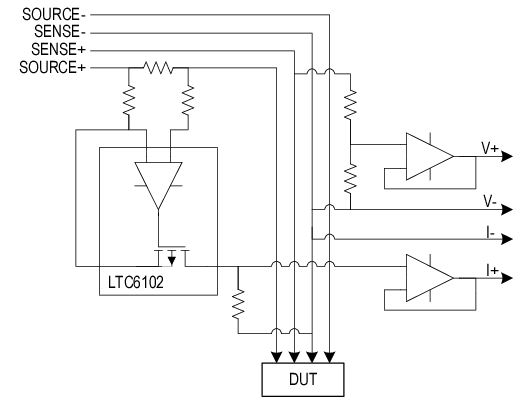
\includegraphics[width=1\linewidth]{img/03/circuit} 

}

\caption[Measurement circuit (simplified) devoted to extract and
adapt the signals to the DAQ input requirements.]{Measurement circuit (simplified) devoted to extract and
adapt the signals to the DAQ input requirements.}\label{fig:circuit}
\end{marginfigure}

Figure \ref{fig:circuit} shows a simplified scheme of this circuit. The
voltage drop in a small and high-precision resistor is amplified to
measure the current signal. At the same time, a resistive divider
couples the voltage signal. Considering that the DAQ card has certain
settling time, it can be modelled as a small capacity which acts as a
low pass filter. Thus, two buffers (voltage followers) are placed before
the DAQ card to decrease the output impedance of the
circuit\cite[0pt]{ni2014}\marginnote{\hypersetup{hidelinks}\color{white}\citet{ni2014}}.

A small command-line tool\footnote{Available at
  \url{https://github.com/Enchufa2/daq-acquire}} was developed to
perform measurements on the DAQ card using the open-source
Comedi\footnote{\url{http://comedi.org}} drivers and libraries.

Regarding the kernel instrumentation, we take advantage of
SystemTap\footnote{\href{(https://sourceware.org/systemtap)}{https://sourceware.org/systemtap}},
an open-source infrastructure around the Linux kernel that dramatically
simplifies information gathering on a running Linux system (kernel,
modules and applications). It provides a scripting language for writing
instrumentation. A SystemTap script is parsed into C code, compiled into
a kernel module and hot-plugged into a live running system.

\hypertarget{measurement-and-uncertainty-analysis}{%
\section{Measurement and Uncertainty
Analysis}\label{measurement-and-uncertainty-analysis}}

The International Vocabulary of Metrology (VIM) defines a
\emph{quantity} as
follows\cite[0pt]{VIM:2012}\marginnote{\hypersetup{hidelinks}\color{white}\citet{VIM:2012}}:

\begin{quote}
\emph{A property of a phenomenon, body, or substance, where the property
has a magnitude that can be expressed as a number and a reference}.
\end{quote}

\noindent where most typically the number is a \emph{quantity value},
attributed to a \emph{measurand} and experimentally obtained via some
measurement procedure, and the reference is a \emph{measurement unit}.

Additionally, any quantity value must accommodate some indication about
the quality of the measurement, a quantifiable attribute known as
\emph{uncertainty} (also traditionally known as \emph{error}). The Guide
to the Expression of Uncertainty in Measurement (GUM) defines
\emph{uncertainty} as
follows\cite[0pt]{GUM:2008}\marginnote{\hypersetup{hidelinks}\color{white}\citet{GUM:2008}}:

\tolerance 0

\begin{quote}
\emph{A parameter, associated with the result of a measurement, that
characterises the dispersion of the values that could reasonably be
attributed to the measurand}.
\end{quote}

\fussy

Uncertainty can be mainly classified into \emph{standard uncertainty},
which is the result of a direct measurement (e.g., electrical voltage
measured with a voltmeter, or current measured with a amperimeter), and
\emph{combined standard uncertainty}, which is the result of an indirect
measurement (i.e., the standard uncertainty when the result is derived
from a number of other quantities by the means of some mathematical
relationship; e.g., electrical power as a product of voltage and
current). Therefore, provided a set of quantities with known
uncertainties, the process of obtaining the uncertainty of a derived
measurement is called \emph{propagation of uncertainty}.

\newthought{Traditionally}, computational systems have treated these
three components (quantity values, measurement units and uncertainty)
separately. Data consisted of bare numbers, and mathematical operations
applied to them solely. Units were just metadata, and error propagation
was an unpleasant task requiring additional effort and complex
operations. Nowadays though, many software libraries have formalised
\emph{quantity calculus} as method of including units within the scope
of mathematical operations, thus preserving dimensional correctness and
protecting us from computing nonsensical combinations of quantities.
However, these libraries rarely integrate uncertainty handling and
propagation\cite[-15mm]{Flatter:2018}\marginnote{\hypersetup{hidelinks}\color{white}\citet{Flatter:2018}}.

Within the R environment, the \texttt{units}
package\cite[0pt]{CRAN:units,Pebesma:2016:units}\marginnote{\hypersetup{hidelinks}\color{white}\citet{CRAN:units,Pebesma:2016:units}}
defines a class for associating unit metadata to numeric vectors, which
enables transparent quantity derivation, simplification and conversion.
This approach is a very comfortable way of managing units with the added
advantage of eliminating an entire class of potential programming
mistakes. Unfortunately, neither \texttt{units} nor any other package
address the integration of uncertainties into quantity calculus.

In the following, we discuss propagation and reporting of uncertainty,
and we present a framework for associating uncertainty metadata to R
vectors, matrices and arrays, thus providing transparent, lightweight
and automated propagation of uncertainty. This implementation also
enables ongoing developments for integrating units and uncertainty
handling into a complete solution.

\hypertarget{propagation-of-uncertainty}{%
\subsection{Propagation of
Uncertainty}\label{propagation-of-uncertainty}}

There are two main methods for propagation of uncertainty: the
\emph{Taylor series method} (TSM) and the \emph{Monte Carlo method}
(MCM). The TSM, also called the \emph{delta method}, is based on a
Taylor expansion of the mathematical expression that produces the output
variables. As for the MCM, it is able to deal with generalised input
distributions and propagates the error by Monte Carlo simulation.

The TSM is a flexible method of propagation of uncertainty that can
offer different degrees of approximation given different sets of
assumptions. The most common and well-known form of TSM is a first-order
TSM assuming normality, linearity and independence. In the following, we
will provide a short description. A full derivation, discussion and
examples can be found in \citet{Arras:1998}.

Mathematically, an indirect measurement is obtained as a function of
\(n\) direct or indirect measurements, \(Y = f(X_1, ..., X_n)\), where
the distribution of \(X_n\) is unknown \emph{a priori}. Usually, the
sources of random variability are many, independent and probably unknown
as well. Thus, the central limit theorem establishes that an addition of
a sufficiently large number of random variables tends to a normal
distribution. As a result, the \emph{first assumption} states that
\(X_n\) are normally distributed.




\begin{marginfigure}[-1in]

{\centering 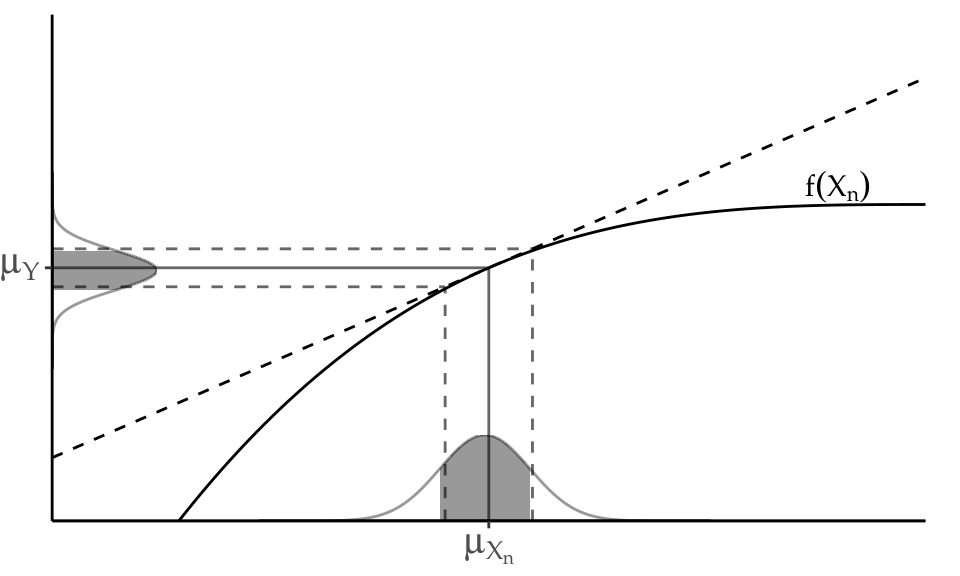
\includegraphics{03-testbed_files/figure-latex/propagation-1} 

}

\caption[Illustration of linearity in an interval \(\pm\) one
standard deviation around the mean.]{Illustration of linearity in an interval \(\pm\) one
standard deviation around the mean.}\label{fig:propagation}
\end{marginfigure}

The \emph{second assumption} presumes linearity, i.e., that \(f\) can be
approximated by a first-order Taylor series expansion around
\(\mu_{X_n}\) (see Figure \ref{fig:propagation}). Then, given a set of
\(n\) input variables \(X\) and a set of \(m\) output variables \(Y\),
the first-order \emph{error propagation law} establishes that
%
\begin{equation}
  \Sigma_Y = J_X \Sigma_X J_X^T \label{eq:assumption2}
\end{equation}
%
where \(\Sigma\) is the covariance matrix and \(J\) is the Jacobian
operator.

\pagebreak

Finally, the \emph{third assumption} supposes independency among the
uncertainty of the input variables. This means that the
cross-covariances are considered to be zero, and the equation above can
be simplified into the most well-known form of the first-order TSM:
%
\begin{equation}
  \left(\Delta y\right)^2 = \sum_i \left(\frac{\partial f}{\partial x_i}\right)^2\cdot \left(\Delta x_i\right)^2 \label{eq:TSM}
\end{equation}
%


In practice, as recommended in the GUM, this first-order approximation
is good even if \(f\) is non-linear, provided that the non-linearity is
negligible compared to the magnitude of the uncertainty, i.e.,
\(\mathbb{E}[f(X)]\approx f(\mathbb{E}[X])\). Also, this weaker
condition is distribution-free: no assumptions are needed on the
probability density functions (PDF) of \(X_n\), although they must be
reasonably symmetric.

\hypertarget{reporting-uncertainty}{%
\subsection{Reporting Uncertainty}\label{reporting-uncertainty}}

The GUM defines four ways of reporting standard uncertainty and combined
standard uncertainty. For instance, if the reported quantity is assumed
to be a mass \(m_S\) of nominal value 100 g:

\begin{quote}
\begin{enumerate}
\def\labelenumi{\arabic{enumi}.}
\tightlist
\item
  \(m_S = 100.02147\) g with (a combined standard uncertainty) \(u_c\) =
  0.35 mg.
\item
  \(m_S = 100.02147(35)\) g, where the number in parentheses is the
  numerical value of (the combined standard uncertainty) \(u_c\)
  referred to the corresponding last digits of the quoted result.
\item
  \(m_S = 100.02147(0.00035)\) g, where the number in parentheses is the
  numerical value of (the combined standard uncertainty) \(u_c\)
  expressed in the unit of the quoted result.
\item
  \(m_S = (100.02147 \pm 0.00035)\) g, where the number following the
  symbol \(\pm\) is the numerical value of (the combined standard
  uncertainty) \(u_c\) and not a confidence interval.
\end{enumerate}
\end{quote}

Schemes (2, 3) and (4) will be referred to as \emph{parenthesis}
notation and \emph{plus-minus} notation respectively. Although (4) is a
very extended notation, the GUM explicitly discourages its use to
prevent confusion with confidence intervals. Throughout this document,
we will be using (2) unless otherwise specified.

\hypertarget{automated-uncertainty-handling-in-r-the-errors-package}{%
\subsection{\texorpdfstring{Automated Uncertainty Handling in R: The
\texttt{errors}
Package}{Automated Uncertainty Handling in R: The errors Package}}\label{automated-uncertainty-handling-in-r-the-errors-package}}

Following the approach of the \texttt{units} package, this thesis
develops a framework for automatic propagation and reporting of
uncertainty: the \texttt{errors}
package\cite[0pt]{R-errors}\marginnote{\hypersetup{hidelinks}\color{white}\citet{R-errors}}.
This R package aims to provide easy and lightweight handling of
measurements with errors, including propagation using the first-order
TSM presented in the previous section and a formally sound
representation. Errors, given as (combined) standard uncertainties, can
be assigned to numeric vectors, matrices and arrays, and then all the
mathematical and arithmetic operations are transparently applied to both
the values and the associated errors. The following example sets a
simple vector with a 5\% of error:

\begin{Shaded}
\begin{Highlighting}[]
\KeywordTok{library}\NormalTok{(errors)}

\NormalTok{x <-}\StringTok{ }\DecValTok{1}\OperatorTok{:}\DecValTok{5}
\KeywordTok{errors}\NormalTok{(x) <-}\StringTok{ }\NormalTok{x }\OperatorTok{*}\StringTok{ }\FloatTok{0.05}
\NormalTok{x}
\end{Highlighting}
\end{Shaded}

\begin{verbatim}
## Errors: 0.05 0.10 0.15 0.20 0.25
## [1] 1 2 3 4 5
\end{verbatim}

The \texttt{errors()} function assigns or retrieves a vector of errors,
which is stored as an attribute of the class \texttt{errors}.
Internally, the package provides S3 methods\footnote{See ``Writing R
  Extensions'' for further details:
  \url{https://cran.r-project.org/doc/manuals/r-release/R-exts.html}}
for the generics belonging to the groups \texttt{Math}, \texttt{Ops} and
\texttt{Summary}, plus additional operations such as subsetting
(\texttt{{[}}, \texttt{{[}\textless{}-}, \texttt{{[}{[}},
\texttt{{[}{[}\textless{}-}), concatenation (\texttt{c()}),
differentiation (\texttt{diff}), row and column binding (\texttt{rbind},
\texttt{cbind}), or coercion to data frame and matrix.

\begin{Shaded}
\begin{Highlighting}[]
\KeywordTok{data.frame}\NormalTok{(x, }\DecValTok{3}\OperatorTok{*}\NormalTok{x, x}\OperatorTok{^}\DecValTok{2}\NormalTok{, }\KeywordTok{sin}\NormalTok{(x), }\KeywordTok{cumsum}\NormalTok{(x))}
\end{Highlighting}
\end{Shaded}

\begin{verbatim}
##         x  X3...x    x.2   sin.x. cumsum.x.
## 1 1.00(5)  3.0(2) 1.0(1)  0.84(3)   1.00(5)
## 2  2.0(1)  6.0(3) 4.0(4)  0.91(4)    3.0(1)
## 3  3.0(2)  9.0(5) 9.0(9)   0.1(1)    6.0(2)
## 4  4.0(2) 12.0(6)  16(2)  -0.8(1)   10.0(3)
## 5  5.0(2) 15.0(8)  25(2) -0.96(7)   15.0(4)
\end{verbatim}

It is worth noting that both values and errors are stored with all the
digits. However, when a single measurement or a column of measurements
in a data frame are printed, the output is properly formatted to show a
single significant digit for the error. This is achieved by providing S3
methods for \texttt{format()} and \texttt{print()}. The
\emph{parenthesis} notation is used by default, but this can be
overridden through the appropriate option in order to use the
\emph{plus-minus} notation instead.

\hypertarget{whole-device-measurements}{%
\section{Whole-Device Measurements}\label{whole-device-measurements}}

Figure \ref{fig:testbed} shows the proposed testbed for whole-device
measurements. It comprises two laptop computers ---the DUT and an access
point (AP)--- and a controller. The controller is a workstation with the
DAQ card installed and it performs the energy measurements. At the same
time, it sends commands to the DUT and AP through a wired connection and
monitors the wireless connection between DUT and AP through a probe.




\begin{figure}

{\centering 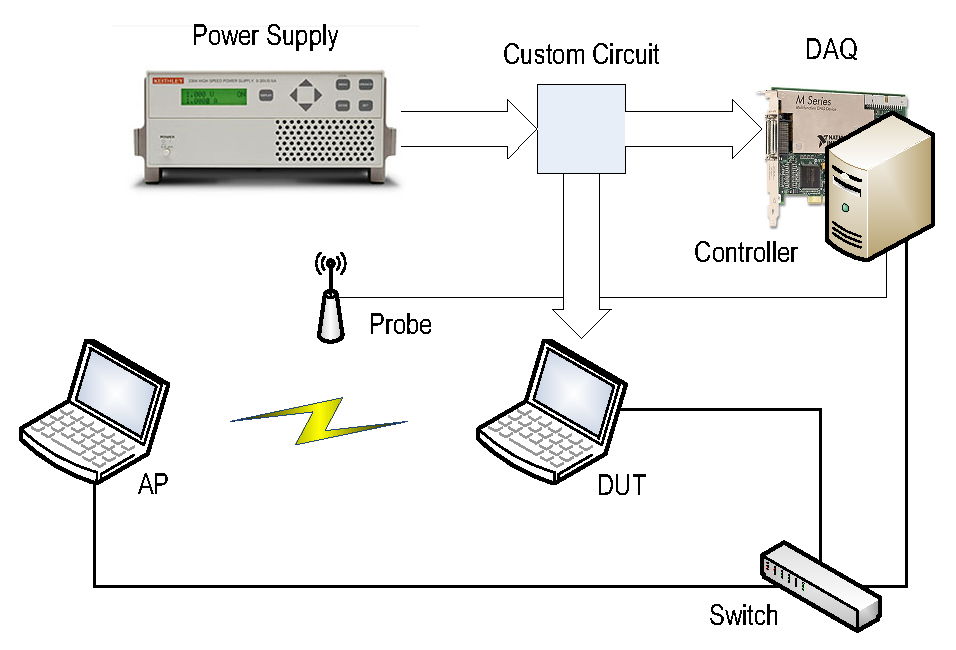
\includegraphics{img/03/testbed} 

}

\caption[Testbed for whole-device energy measurements. The
\emph{custom circuit} is the one sketched in Figure \ref{fig:circuit}.]{Testbed for whole-device energy measurements. The
\emph{custom circuit} is the one sketched in Figure \ref{fig:circuit}.}\label{fig:testbed}
\end{figure}

\newthought{The experimental methodology} to characterise the DUT's
energy parameters is as follows. Given a collection of network parameter
values (modulation coding scheme or MCS, transmission power, packet
size, framerate), we run steady experiments for several seconds in order
to gather averaged measures. Each experiment comprises the steps shown
in Figure \ref{fig:sequence}.




\begin{marginfigure}

{\centering 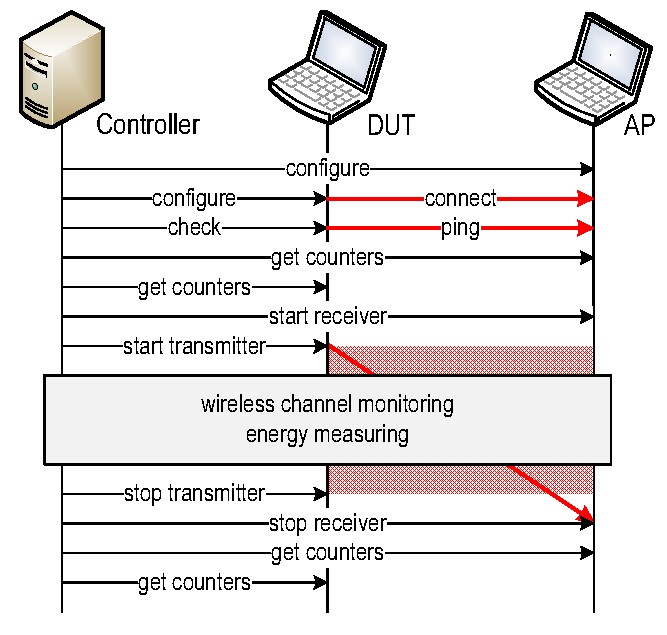
\includegraphics[width=1\linewidth]{img/03/sequence} 

}

\caption[Measurement methodology. Time sequence of a whole-device
experiment.]{Measurement methodology. Time sequence of a whole-device
experiment.}\label{fig:sequence}
\end{marginfigure}

\begin{enumerate}
\def\labelenumi{\arabic{enumi}.}
\tightlist
\item
  AP and DUT are configured. The DUT connects to the wireless network
  created by the AP and checks the connectivity. Setting up this network
  in a clear channel is highly advisable to avoid interference. The 5
  GHz band, with an 802.11a-capable card, has good candidates.
\item
  The packet counters of the wireless interfaces are saved for later
  use.
\item
  Receiver and transmitter are started. We use the
  \texttt{mgen}\footnote{\url{http://cs.itd.nrl.navy.mil/work/mgen}}
  traffic generator and a simple \texttt{netcat} at the receiver.
\item
  The controller monitors the wireless channel and collects an energy
  trace that will be averaged later.
\item
  Transmitter and Receiver are stopped.
\item
  Because of the unreliability of the wireless medium, the packet
  counters, together with the monitoring information, are used to ensure
  that the experiment was successful (i.e., the traffic seen agrees with
  the configured parameters).
\end{enumerate}

\hypertarget{validation}{%
\subsection{Validation}\label{validation}}

In order to validate our measurement framework, several experiments were
performed with one of the devices studied in \citet{Serrano2014} as DUT.
We selected the Soekris net4826-48 equipped with an Atheros AR5414-based
802.11a/b/g Mini-PCI card because it is the one with the largest
cross-factor. The operating system (OS) was Linux Voyage with kernel
2.6.30 and the MadWifi driver v0.9.4.

The first task was to perform the energy breakdown given in
\citet{Serrano2014} in transmission mode:

\begin{description}
\tightlist
\item[User space]
The Soekris generates packets using \texttt{mgen}, but they are
discarded before being delivered to the OS, by using the \texttt{sink}
device rather than \texttt{udp}.
\item[Kernel space]
Packets cross the network stack and are discarded in the driver, by
commenting the \texttt{hardstart} MadWifi command that performs the
actual delivery of the frame to the wireless network interface card
(NIC).
\item[Wireless NIC]
Packets are transmitted, i.e., are delivered to the wireless medium.
\end{description}

The NoACK functionality from 802.11e was activated in order to avoid ACK
receptions. Therefore, Equation \eqref{eq:new-energy-model} can be
simplified as follows to describe complete transmissions:
%
\begin{equation*}
 \overline{P}(\tau, \lambda) = \rho_{id} + \rho_{tx}\tau + \gamma_{xg}\lambda
 \label{eq:validation1}
\end{equation*}
%


Figure \ref{fig:validation1} represents the equation above (red lines)
and depicts how the energy toll splits across the processing chain with
different parameters (blue and green lines). The dashed line depicts the
idle consumption as a reference, \(\rho_{id}=3.65(1)\) W.





\begin{marginfigure}[-3.5in]

{\centering 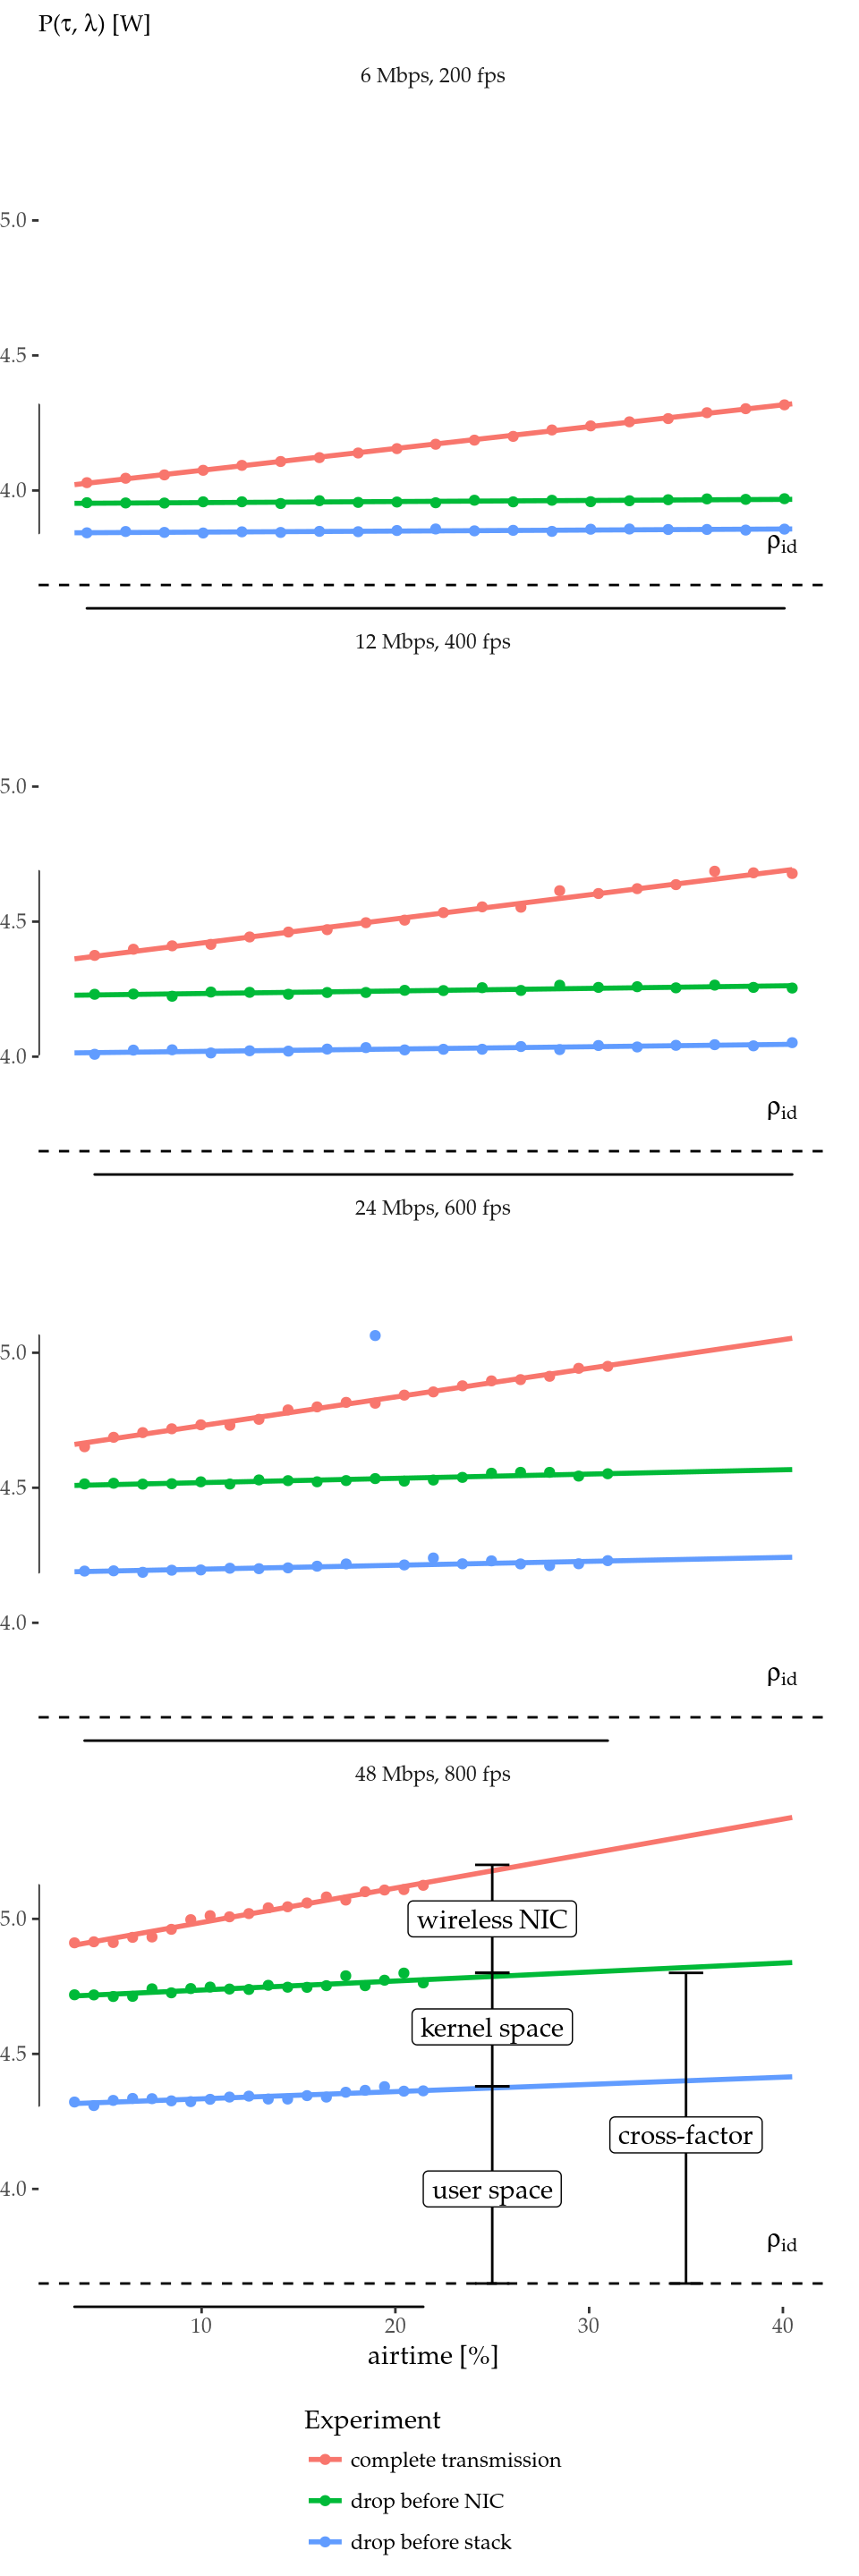
\includegraphics{03-testbed_files/figure-latex/validation1-1} 

}

\caption[Power consumption breakdown vs.~airtime.]{Power consumption breakdown vs.~airtime.}\label{fig:validation1}
\end{marginfigure}

\begin{figure}[b]

{\centering 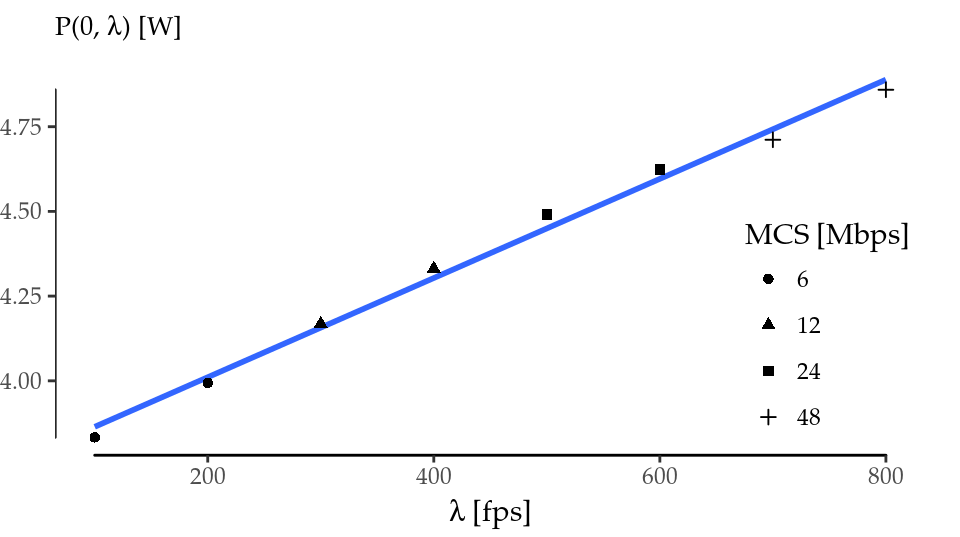
\includegraphics{03-testbed_files/figure-latex/validation2-1} 

}

\caption[Power consumption offset (\(\tau=0\)) vs.~framerate.]{Power consumption offset (\(\tau=0\)) vs.~framerate.}\label{fig:validation2}
\end{figure}

Indeed, these results are quite similar to \citet{Serrano2014} and
confirm that the cross-factor accounts for the largest part of the
energy consumption. Moreover, \citet{Serrano2014} reports that the
cross-factor is \emph{almost} independent of the packet size.
Interestingly, our results have captured a small dependence that can be
especially observed in the 600 fps case.

Finally, we can derive the cross-factor value and compare it. Taking the
offset of the red regression lines of Figure \ref{fig:validation1}, we
can plot Figure \ref{fig:validation2} and fit these points with
\(\tau=0\). This regression yields the values \(\rho_{id}=3.72(4)\) W
(\(3.65(1)\) W measured) and \(\gamma_{xg}=1.46(7)\) mJ, quite close to
the values reported in \citet{Serrano2014}.

\hypertarget{per-component-measurements}{%
\section{Per-Component Measurements}\label{per-component-measurements}}

Figure \ref{fig:testbed-card} shows the proposed testbed for
per-component measurements. The component (a wireless card) is attached
to the device through a flexible x1 PCI Express to Mini PCI Express
adapter from Amfeltec. This adapter connects the PCI bus' data channels
to the host and provides an ATX port so that the wireless card can be
supplied by an external power source.



\begin{marginfigure}

{\centering 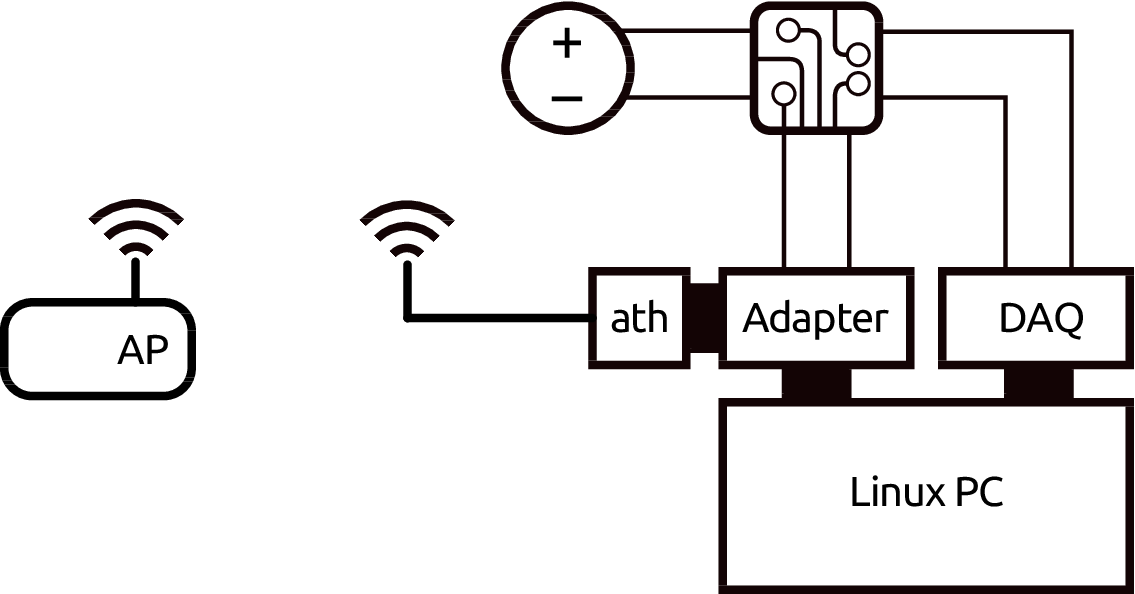
\includegraphics[width=1\linewidth]{img/03/testbed-card} 

}

\caption[Testbed for per-component energy measurements.]{Testbed for per-component energy measurements.}\label{fig:testbed-card}
\end{marginfigure}

Here, the same PC holds the DAQ card. In this way, the operations sent
to the wireless card and the energy measurements can be correlated using
the same timebase, which is required for the next section. For other
type of experiments, this requirement can be relaxed, and the DAQ card
can be hosted in a separate machine.

\hypertarget{characterisation-of-a-cots-device}{%
\subsection{Characterisation of a COTS
Device}\label{characterisation-of-a-cots-device}}

\hypertarget{state-consumption-parametrisation}{%
\paragraph{State Consumption
Parametrisation}\label{state-consumption-parametrisation}}
\addcontentsline{toc}{paragraph}{State Consumption Parametrisation}

In the following, we demonstrate a complete state parametrisation (power
consumption in transmission, reception, overhearing, idle and sleep) of
a commercial off-the-shelf (COTS) card: an Atheros AR9280-based
802.11a/b/g/n Half Mini-PCI Express card. All measurements (except for
the sleep state) were taken with the wireless card associated to the AP
in 11a mode to avoid any interfering traffic, and it was placed very
close to the node to obtain the best possible signal quality. The
reception of beacons is accounted in the baseline consumption (idle).

The card under test performed transmissions/receptions to/from the AP at
a constant rate and with fixed packet length. In order to avoid
artifacts from the reception/transission of ACKs, UDP was used and the
NoACK policy was enabled. Packet overhearing was tested by generating
traffic of the same characteristics from a secondary STA placed in the
same close range (\(\sim\)cm). Under these conditions, several values of
airtime percentage were swept. For each experiment, current and voltage
signals were sampled at 100 kHz and the average power consumption was
measured with a basic precision of 1 mW over intervals of 3 s.

\pagebreak

Regarding the sleep state, the card's \texttt{ath9k} driver internally
defines three states of operation: \emph{awake}, \emph{network sleep}
and \emph{full sleep}. A closer analysis reveals that the card is
\emph{awake}, or in \emph{active state}, when it is operational (i.e.,
transmitting, receiving or in idle state, whether as part of an SSID or
in monitor mode), and it is in \emph{full sleep} state when it is not
operational at all (i.e., interface down or up but not connected to any
SSID). The \emph{network sleep} state is used by the 802.11 Power Save
(PS) mechanism, but essentially works in the same way as \emph{full
sleep}, that is, it turns off the main reference clock and switches to a
secondary 32 kHz one. Therefore, we saw that \emph{full sleep} and
\emph{network sleep} are the same state in terms of energy: they consume
exactly the same power. The only difference is that \emph{network sleep}
sets up a tasklet to wake the interface periodically (to receive the
traffic indication map), as required by the PS mode.



\begin{figure}

{\centering 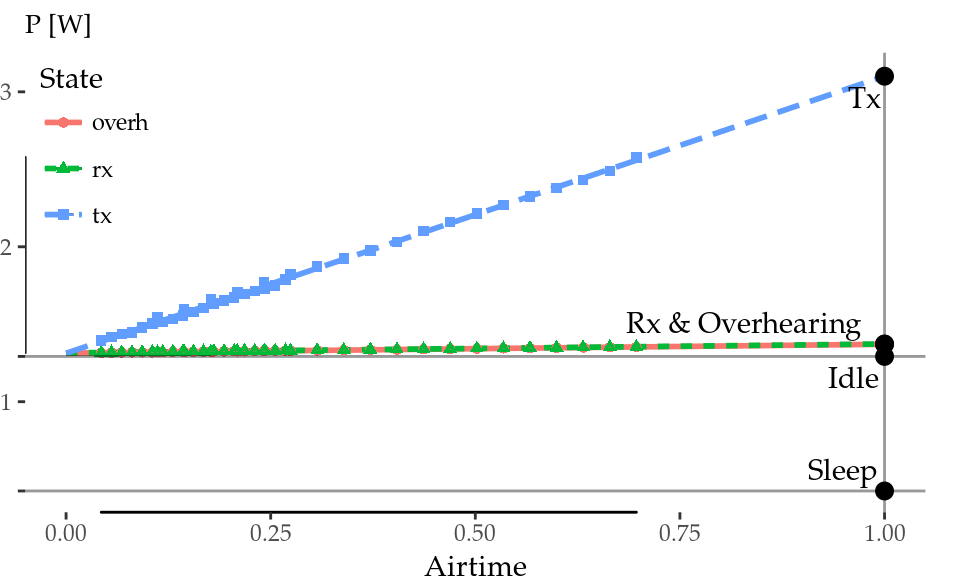
\includegraphics{03-testbed_files/figure-latex/power-1} 

}

\caption[Atheros AR9280 power consumption in 11a mode.]{Atheros AR9280 power consumption in 11a mode.}\label{fig:power}
\end{figure}

Figure \ref{fig:power} shows our results for transmission, reception and
overhearing. Idle and sleep consumptions were measured independently,
are depicted with gray horizontal lines for reference. As expected,
power consumptions in transmission/reception/overhearing state are
proportional to airtime, thus the power consumption of such operations
can be easily estimated by extrapolating the regression line to the
100\% of airtime (gray vertical line).

These average values are shown in Table \ref{tab:powert}. First of all,
reception and overhearing consumptions are the same within the error,
and they are close to idle consumption. Transmission power is more than
two times larger than reception. Finally, the sleep state saves almost
the 70\% of the energy compared to idle/reception.

\begin{table}

\begin{center}
\begin{tabular}{rcccl}
\toprule
State & Mode & Channel & MHz & Power [W]\\
\midrule
Transmission &  &  &  & 3.10(2)\\

Reception &  &  &  & 1.373(1)\\

Overhearing &  &  &  & 1.371(1)\\

Idle & \multirow{-4}{*}{\centering\arraybackslash 11a} & \multirow{-4}{*}{\centering\arraybackslash 44} & \multirow{-4}{*}{\centering\arraybackslash 20} & 1.292(2)\\
\cmidrule{1-5}
Sleep & - & - & - & 0.424(2)\\
\cmidrule{1-5}
 &  &  & 20 & 1.137(4)\\

\multirow{-2}{*}{\raggedleft\arraybackslash Idle} & \multirow{-2}{*}{\centering\arraybackslash 11n} & \multirow{-2}{*}{\centering\arraybackslash 11} & 40 & 1.360(4)\\
\bottomrule
\end{tabular}
\end{center}
\caption{\label{tab:powert}Atheros AR9280 power consumption.}
\end{table}

\hypertarget{downclocking-consumption-characterisation}{%
\paragraph{Downclocking Consumption
Characterisation}\label{downclocking-consumption-characterisation}}
\addcontentsline{toc}{paragraph}{Downclocking Consumption
Characterisation}

As the AR9280's documentation states, its reference clock runs at 44 MHz
for 20 MHz channels and at 88 MHz for 40 MHz channels in the 2.4 GHz
band, and at 40 MHz for 20 MHz channels and at 80 MHz for 40 MHz
channels in the 5 GHz band. Thus, as Table \ref{tab:powert} shows, we
measured two more results to gain additional insight into the behaviour
of the main reference clock, which is known to be
linear\cite[0pt]{Zhang2012}\marginnote{\hypersetup{hidelinks}\color{white}\citet{Zhang2012}}.

Using an 11n-capable AP, we measured the idle power in the 2.4 GHz band
with two channel widths, 20 and 40 MHz. Note that the idle power in 11a
mode (5 GHz band), with a 40 MHz clock, is higher than the idle power
with a 44 MHz clock. This is because both bands are not directly
comparable, as the 5 GHz one requires more amplification (the effect of
the RF amplifier is out of the scope of this work).

With these two points, we can assume a higher error (of about 10 mW) and
try to estimate a maximum and a minimum slope for the power consumed by
the main clock as a function of the frequency \(f\). The resulting
averaged regression formula is the following:
%
\begin{equation}
 P(f) = 0.91(3) + 0.0051(5)f \label{eq:Pf}
\end{equation}
%


This result, although coarse, enables us to estimate how a downclocking
approach should perform in COTS devices. It shows that the main
consumption of the clock goes to the baseline power (the power needed to
simply turn it on), and that the increment per MHz is low: 5.1(5)
mW/MHz. As a consequence, power-saving mechanisms based on idle
downclocking, such as the one developed by \citet{Zhang2012}, will not
save too much energy compared to the sleep state of COTS devices. For
instance, the x16 downclocking achieved by this mechanism applied to
this Atheros card throws an idle power consumption of 1.10(2) W in 11a
mode, i.e., about a 15\% of saving according to Table \ref{tab:powert},
which is low compared to the 70\% of its sleep state. This questions the
effectiveness of complex schemes based on downclocking compared to
simpler ones based on the already existing sleep state.

\hypertarget{summary}{%
\section{Summary}\label{summary}}

We have built and validated a comprehensive, high-accuracy and
high-precision energy measurement framework, which is capable of
measuring a wide range of wireless devices, as well as multiple
heterogeneous devices synchronously. Rigorous experimental methodologies
have been introduced to characterise the energy parameters of devices
and wireless components. Based on these, the framework has been
validated against previous results from \citet{Serrano2014}, and a COTS
wireless card, which will be used in further experiments throughout this
thesis, has been studied and parametrised.

At the same time, measurement handling has been systematised into
\texttt{errors}\cite[0pt]{contrib-03}\marginnote{\hypersetup{hidelinks}\color{white}\citet{contrib-03}},
a lightweight R package for managing numeric data with associated
standard uncertainties. The new class \texttt{errors} provides numeric
operations with automated propagation of uncertainty through a
first-order TSM, and a formally sound representation of measurements
with errors. Using this package makes the process of computing indirect
measurements easier and less error-prone.

Future work includes importing and exporting data with uncertainties,
and providing the user with an interface for plugging uncertainty
propagation methods from other packages. Finally, \texttt{errors}
enables ongoing developments\footnote{\emph{Quantities for R}, a project
  funded by the R Consortium (see
  \url{https://www.r-consortium.org/projects/awarded-projects})} for
integrating \texttt{units} and uncertainty handling into a complete
solution for quantity calculus. Having a unified workflow for managing
measurements with units and errors would be an interesting addition to
the R ecosystem with very few precedents in other programming languages.

\hypertarget{ch:04}{%
\chapter{Deseeding Energy Consumption of Network Stacks}\label{ch:04}}

\newthought{The cross-factor} is a per-frame energy toll that can be
ascribed to the fact that every frame received or transmitted through a
wireles interface requires some processing in the device's network
stack. The aim of this chapter is to break down the cross-factor into
its constituent parts in order to comprehend the underlying causes, all
within the scope of providing an accurate mathematical description of
the cross-factor which would give the energy model an unprecedented
specificity. This may enable us to evaluate old energy efficiency
strategies and to propose and test new schemes, both at a device and at
a network level.

Our proposal, with respect to the work by \citet{Serrano2014}, is to
switch to a more generic target platform, which will provide us an easy
access to powerful kernel instrumentation, as described in the previous
chapter, present in most general-purpose Linux-based distributions.

To be able to conduct fine-grained energy debugging of the network
stack, we must somehow isolate the network activity from the consumption
of the rest of the system. To this aim, the next section is devoted to
dissect and discuss the components of a laptop computer in order to
understand their implications in the global power consumption, and how
to minimise their impact. Then, subsequent sections explore the roots of
the cross-factor.

\hypertarget{anatomy-of-a-laptop-computer}{%
\section{Anatomy of a Laptop
Computer}\label{anatomy-of-a-laptop-computer}}

A laptop computer is a complex and power-hungry piece of hardware. It
comprises a number of components, both hardware (battery, screen, hard
disk drive, fan, wireless card, RAM memory, CPU) and software (services,
kernel, drivers), that require a thorough discussion. Some of them are
not present in other devices (e.g., the fan), and some others are
essentially different in terms of performance and power requirements.

\hypertarget{battery}{%
\paragraph{Battery}\label{battery}}
\addcontentsline{toc}{paragraph}{Battery}

The battery is a serious obstacle for energy measurements. Although
using it as power source is actually possible, it is totally impractical
because it prevents long term experiments, and the constant need for
recharging is a waste of time. Then, the use of an external power source
is highly advisable, but in this case the battery must be removed to
avoid noise coming from battery charging and discharging.

Nevertheless, usually supplying DC power through the power jack socket
is not enough. Most manufacturers are interested in forcing the user to
acquire and use original parts. As a consequence, most laptops are
capable of detecting the AC adapter and take unexpected\footnote{That
  is, unexpected\ldots{} for the user.} decisions. This is generally
done through a third connection in the power jack. For example, in the
case of Dell computers, this third wire goes to a transistor-shaped
component placed in the AC transformer. Actually, this component is a
small memory that can be read using a 1-wire protocol. It stores a
serial number that identifies the AC adapter.

Summing up, if the laptop does not detect this memory, the BIOS can do
improper\footnote{Again, improper\ldots{} from the user's standpoint.}
things. For instance, we detected that Dell computers' BIOS do not allow
the OS to control CPU frequency scaling. Fortunately, it is very
straightforward to \emph{borrow} such a component from an official AC
adapter and attach it permanently to the third connection of the power
jack socket. In this way, any power source looks as an original part to
the BIOS, and the OS kernel can freely manage all the system's
capabilities.

\hypertarget{screen}{%
\paragraph{Screen}\label{screen}}
\addcontentsline{toc}{paragraph}{Screen}

Same as for
smartphones\cite[0pt]{Carroll2010}\marginnote{\hypersetup{hidelinks}\color{white}\citet{Carroll2010}},
the screen is the most energy-hungry component in a laptop computer. It
typically accounts for more than a half of the total energy consumed
when the computer is just powered on and idling. Thus, the screen
constitutes a very high and variable (as it depends on the GPU activity)
baseline consumption that must be avoided in wireless experiments. In
Linux, this can be done by finding the backlight device entry in the
\texttt{/sys/class} subsystem and simply resetting it, so that the
screen is permanently powered off.

\hypertarget{hard-disk-drive}{%
\paragraph{Hard Disk Drive}\label{hard-disk-drive}}
\addcontentsline{toc}{paragraph}{Hard Disk Drive}

Regarding the system's non-volatile memory, we cannot get rid of it
because it is needed for the OS storage. Commonly, laptops are equipped
with hard disk drives (HDD), which are mechanical devices powered with
voltages ranging from 5 to 12 V. HDDs are proven to be energy-hungry
devices\cite[-1cm]{Hylick2008}\marginnote{\hypersetup{hidelinks}\color{white}\citet{Hylick2008}}
with a consumption variability in ascending order of tens of Watts. As a
consequence, every read/write during an experiment generates an
intractable noise.

On the other hand, all the devices studied in \citet{Serrano2014} use
flash memories. This kind of non-volatile memory is the best option,
because its consumption variability is three orders of magnitude below
HDD's\cite[0pt]{Grupp2009}\marginnote{\hypersetup{hidelinks}\color{white}\citet{Grupp2009}}.
In our experiments, we replaced the original HDD by a solid-state disk
(SSD). Given that an SSD is composed of NAND flash units, its
consumption is much smaller and far more stable.

\hypertarget{fan}{%
\paragraph{Fan}\label{fan}}
\addcontentsline{toc}{paragraph}{Fan}

The thermal characteristics of a laptop computer require a cooling
subsystem: heat sinks (CPU and GPU), air ducts and typically one fan (at
least). The fan is regulated dynamically with a pulse-width modulation
(PWM) technique. This component becomes an unpredictable source of
electrical noise, as its operation point depends on the computer's
thermal state.

Suppressing the fan is not an option because, at some point, the CPU
will heat and the computer will turn off. Our solution was to set it at
fixed medium speed with the help of the \texttt{i8k} kernel module and
the \texttt{i8kfan} user-space application.

\hypertarget{wireless-card}{%
\paragraph{Wireless Card}\label{wireless-card}}
\addcontentsline{toc}{paragraph}{Wireless Card}

This is the last part of the wireless transmission chain and the first
of the reception one. In principle, the energy models in the literature
assure us that a linear behaviour is expected, independently of the
manufacturer or model. However, there are a couple of factors that may
lead us to select a particular card.

\begin{description}
\tightlist
\item[Supported capabilities]
Nowadays, it is very difficult to perform interference-free wireless
experiments over ISM bands without an anechoic chamber\footnote{Especially
  when all your fellows work in similar research topics.}. The 2.4 GHz
band is typically overcrowded, while in the 5 GHz band we have better
chances to find a clear channel. Thus, an 802.11a-capable card is
advisable.
\item[Manufacturer]
Distinct manufacturers (and models) have better or worse driver support
in the Linux kernel. For instance, Intel PRO/Wireless cards are known
for requiring a binary firmware to operate. On the other hand, Atheros
released some source from their binary HAL to help the open-source
community add support for their chips. As a result, there are completely
free and open-source \emph{FullMAC}\footnote{See
  \url{https://wireless.wiki.kernel.org/en/developers/documentation/glossary}
  for the definition of \emph{FullMAC} and \emph{SoftMAC} drivers.}
drivers available for all Atheros chipsets.
\end{description}

All our experiments were conducted using the Atheros AR9280-based
802.11a/b/g/n Half Mini-PCI Express card that was characterised in
Section \ref{characterisation-of-a-cots-device}.

\hypertarget{ram-memory}{%
\paragraph{RAM Memory}\label{ram-memory}}
\addcontentsline{toc}{paragraph}{RAM Memory}

The random-access memory is a fundamental peripheral device in a
computer system: it holds the instructions of the running programs
---the OS kernel included--- and the data associated. Therefore, our
first guess was that the RAM memory could play a meaningful role in the
energy consumption of a wireless communication.

\hypertarget{cpu}{%
\paragraph{CPU}\label{cpu}}
\addcontentsline{toc}{paragraph}{CPU}

The CPU is another power-hungry component. For many years, the first
CPUs were like bulbs: they were consuming the same power whether they
were doing something useful or not. In fact, they executed \emph{junk
code} (i.e., a loop of NOPs) during idle time. Later, CPU architects
realised that more intelligent things can be done in such periods of
time (for instance, enabling some kind of energy-saving mechanism).



\begin{marginfigure}

{\centering 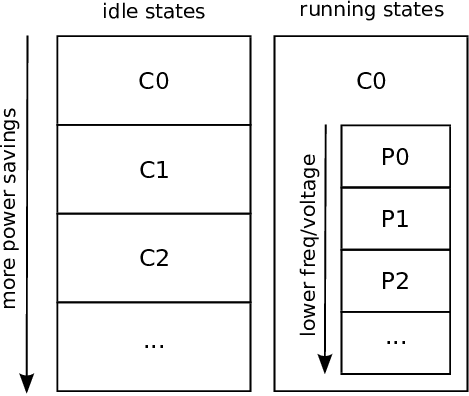
\includegraphics[width=1\linewidth]{img/04/states} 

}

\caption[CPU P- and C-states.]{CPU P- and C-states.}\label{fig:states}
\end{marginfigure}

Nowadays, CPUs are becoming more and more complex. Without seeking to be
exhaustive, a modern CPU has arithmetic control units (ALUs), pipelines,
a control unit, registers, several levels of cache, some clocks,
etcetera. But more interestingly, modern CPUs implement several power
management mechanisms (see Figure \ref{fig:states}), which are covered
by the Advanced Configuration and Power Interface (ACPI).

\begin{description}
\tightlist
\item[P-states]
Also known as \emph{frequency scaling}. When the CPU is running (i.e.,
executing instructions), one of these states apply. P0 means maximum
power and frequency. As Px increases, the voltage is lower and, thus,
the frequency of the clock, and thus the energy consumed, is scaled
down.
\item[C-states]
When the CPU is idle, it enters a Cx state. C0 means maximum power,
because junk code is being executed. This can be a little bit confusing
because, as Figure \ref{fig:states} shows, the CPU is also in C0 when it
is running. In general, C0 means \emph{the CPU is busy doing something},
whether executing actual programs (running) or something not useful
(idle). In C1, the CPU is halted, and can return to an executing state
almost instantaneously. In C2, the main clock is stopped and, as Cx
increases, more and more functional units are shut off. As a
consequence, returning from a deep C-state is very expensive in terms of
latency.
\end{description}

For example, Intel Haswell processors support up to eight C-states: C1,
C1E, C3, C6, C7s, C8, C9, C10. However, the BIOS just reports two
C-states to the ACPI driver, which are called C1 and C2. We have
verified, by comparing idle consumptions for each C-state, that the
correspondence is as follows:

\begin{itemize}
\tightlist
\item
  ACPI C1 corresponds to Intel C1: the CPU is halted and stops executing
  instructions when it enters into idle mode.
\item
  ACPI C2 corresponds to Intel C6: this is a new sleep state introduced
  in the Haswell architecture.
\end{itemize}

Finally, multicore systems introduce additional complexity, because the
OS decides how many cores become active at any time, and each core has
its own power management subsystem (i.e., P- and C-states). Therefore,
our experiments are always carried out in single-core mode to simplify
the analysis.

\hypertarget{services}{%
\paragraph{Services}\label{services}}
\addcontentsline{toc}{paragraph}{Services}

There may be a lot of active user-space services (also called
\emph{daemons}) in a Linux system by default. They can add noise to our
measurements in two ways: by consuming CPU time and writing logs to
disk. Hence, identifying and disabling not essential services is
desirable.

\hypertarget{kernel}{%
\paragraph{Kernel}\label{kernel}}
\addcontentsline{toc}{paragraph}{Kernel}

There exist two power management subsystems for each CPU in the Linux
kernel: \texttt{cpufreq}\footnote{\url{https://www.kernel.org/doc/Documentation/cpu-freq}}
controls P-states and \texttt{cpuidle}\footnote{\url{https://www.kernel.org/doc/Documentation/cpuidle}}
controls C-states. Both subsystems have a similar architecture,
separating mechanism (driver\footnote{It provides the platform-dependent
  state detection capability and the mechanisms to support entry/exit
  into/from different states. By default, there exists an ACPI driver
  that implements standard APIs. Usually, CPU-specific drivers are
  capable of detecting more states than ACPI-compliant ones.}) from
policy (governor\footnote{It is an algorithm that takes in several
  system parameters as input and decides the state to activate.}).

\begin{description}
\tightlist
\item[The \texttt{cpufreq} governor]
has several policies that focus on certain P-states or frequencies to
the detriment of others, e.g., \texttt{performance} (high frequencies)
or \texttt{powersave} (low frequencies). It is also possible to manually
fix certain frequency or range of frequencies.
\item[The \texttt{cpuidle} governor]
takes in the next timer event as main input. Each C-state has a certain
energy cost and exit latency. Thus, intuitively there are two decision
factors that the governor must consider: the energy break-even point and
the performance impact. The next timer event is a good predictor in many
cases, but not perfect since there are other sources of wake-ups (e.g.,
interrupts). Therefore, it computes a correction factor using an array
of 12 independent factors through a running average. Moreover, it is
possible to manually disable the C-states (excepting C0).
\end{description}

\hypertarget{drivers}{%
\paragraph{Drivers}\label{drivers}}
\addcontentsline{toc}{paragraph}{Drivers}

All Linux drivers are compiled as separate modules. In particular,
wireless drivers\footnote{\url{http://wireless.kernel.org}}, along with
the entire 802.11 subsystem, can be compiled out-of-tree within the
\emph{backports} project\footnote{\url{https://backports.wiki.kernel.org}}.
This is very useful in order to use the latest drivers on older kernels.

The wireless driver module interacts directly with the network interface
controller (NIC). In our case, the selected card uses the \texttt{ath9k}
driver. The function \texttt{ath9k\_tx()} is the entry point for the
transmission path. The driver fills the transmission descriptors, copies
the buffer into the NIC memory and sets up several registers that
trigger the transmission.

\newthought{In order to conduct} energy breakdowns like the one depicted
in Figure \ref{fig:validation1}, \citet{Serrano2014} claim that their
methodology discards packets \emph{right after the driver}. This
statement becomes uncertain when a closer look at any wireless driver is
taken. According to our experiments, discarding a frame \emph{before}
the buffer is copied into the NIC implies that \emph{only} half of the
driver is actually taken into account for the cross-factor value. On the
other hand, if we try to discard it in the very last instruction of the
driver (i.e., avoiding setting the register that triggers the hardware
transmission), then the module crashes if the NIC's memory is not
cleaned up, a non-trivial task that anyway would consume more energy.
Due to this, and combined to the fact that drivers differ greatly from
one to another, we do not include the driver into the definition of
cross-factor, given the difficulty of isolating driver and NIC
consumptions.

As with the variety of drivers mentioned above, a similar argument can
be wield against the user-space consumption. Therefore and from here on,
we define \emph{kernel cross-factor} as the energy consumed from the
system call that delivers the message until the driver is reached.
\emph{Cross-factor}, as is, maintains the original definition given by
\citet{Serrano2014} to avoid confusion.

We would also like to highlight that our way of interrupting the
transmission path by discarding a frame in the driver is a bit different
from \citet{Serrano2014}. They conducted this breakdown by commenting a
driver function. This method implies the need for recompiling the
driver, which is time-consuming and not very portable\footnote{Think,
  for instance, about a similar task for a function contained in the
  kernel core.}.

For our part, we generate packets with a short string at the beginning
of packet payloads. The presence of this \emph{magic string} triggers
the packet drop. Our method, despite introducing a very small overhead,
is agile and portable (for instance, it can be implemented on the fly
using SystemTap).

\newthought{The laptop computer} selected for our experiments is a Dell
Latitude E5540 with Intel Core i5-4300U CPU at 1.9 GHz and 8 GB of
SODIMM DDR3 RAM at 1.6 GHz, equipped with an Atheros AR9280-based
802.11a/b/g/n Half Mini-PCI Express card. In our measurements, we use
Fedora-default pre-compiled kernels. We arranged two separate
partitions: one with Fedora 12 and kernel version 2.6.32 and the other
with Fedora 20 and kernel 3.14. Only the latter supports Intel-specific
drivers, thus we use ACPI drivers only in order to operate under similar
conditions.

\hypertarget{cross-factor-separating-the-wheat-from-the-chaff}{%
\section{Cross-Factor: Separating the Wheat from the
Chaff}\label{cross-factor-separating-the-wheat-from-the-chaff}}

We have identified the two main components suspected of being
responsible of the cross-factor: CPU and RAM memory. Our first priority
is to isolate and quantify the impact of the RAM. It is not possible to
regulate its activity, but this can be done for the CPU. For this
purpose, the CPU was fixed at P0-C0 states, i.e., always running at
maximum frequency, maximum energy consumption. We performed an energy
breakdown using this configuration in kernel 3.14 and the results are
shown in Figure \ref{fig:c0}.



\begin{figure*}

{\centering 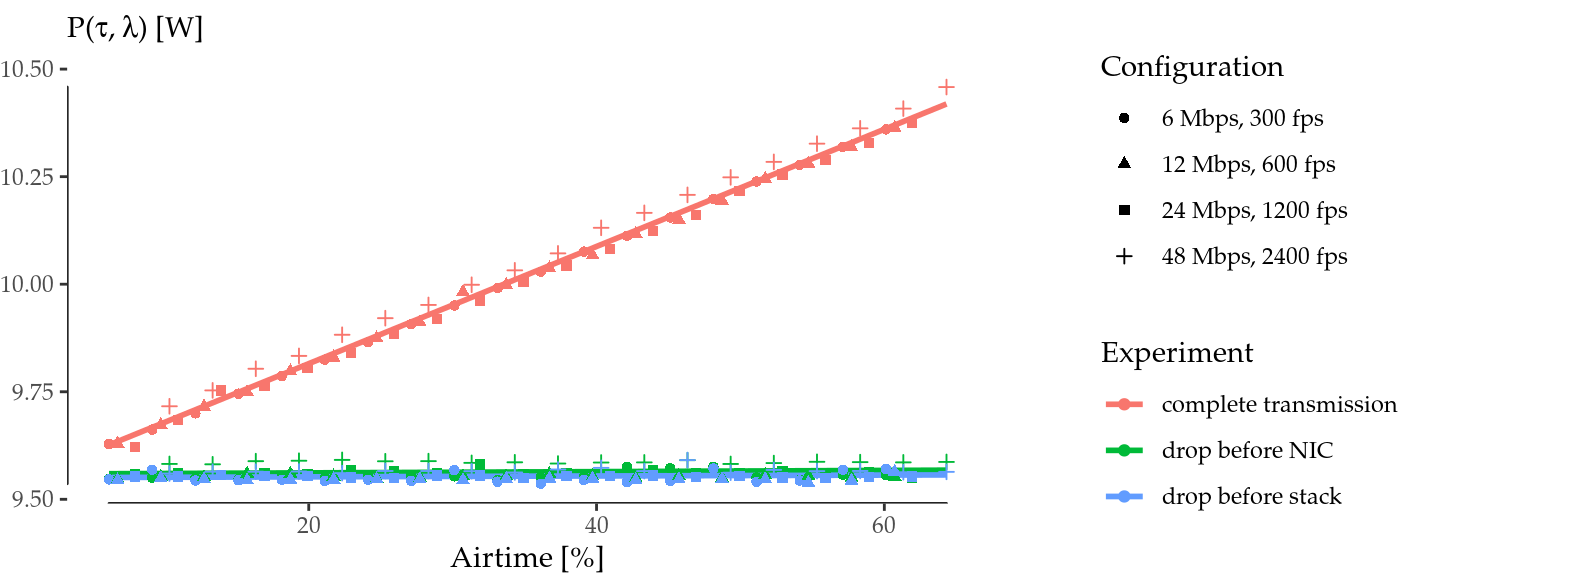
\includegraphics{04-netstacks_files/figure-latex/c0-1} 

}

\caption[Energy breakdown with the CPU fixed at P0-C0 states.]{Energy breakdown with the CPU fixed at P0-C0 states.}\label{fig:c0}
\end{figure*}

The lines appear superimposed: the laptop is consuming the same power
among different parameters, different packet rates. Hence, one important
conclusion to be drawn is that the RAM memory has no significant impact
in the overall energy consumption of wireless transmissions. The noise
can be ascribed to the fact that not all the instructions consume
exactly the same
energy\cite[0pt]{Tiwari1996}\marginnote{\hypersetup{hidelinks}\color{white}\citet{Tiwari1996}}.
Other possible sources of noise are cache and pipeline flushes.

With this simple experiment, we have demonstrated that the CPU is the
leading cause of cross-factor in laptops, and it is clear that the
\texttt{cpuidle} subsystem has a central role, because a CPU spends most
of the time in idle
mode\cite[0pt]{Barroso2007}\marginnote{\hypersetup{hidelinks}\color{white}\citet{Barroso2007}}.
From now on, and in order to take a deeper look at C-states, we remove a
variable by keeping the P-state fixed at P0 (maximum frequency).

\hypertarget{power-consumption-in-unattended-idle-mode}{%
\section{Power Consumption in Unattended Idle
Mode}\label{power-consumption-in-unattended-idle-mode}}

The Soekris net4826-48 used in Section \ref{validation} is equipped with
an AMD Geode SC1100 CPU that supports ACPI C1, C2 and C3
states\footnote{\url{http://datasheets.chipdb.org/upload/National/SC1100.pdf}}.
Unfortunately, it seems that Linux distributions for embed devices, such
as Voyage Linux, disable \texttt{cpuidle} in their kernels, which means
that the OS has no control over the idle mode. In such conditions, we
know now that the CPU cannot be in C0 all the time, because the device
does not consume the same power with different parameters. What is
happening then?

\newthought{Back to our laptop}, it is possible to disable
\texttt{cpuidle} through the kernel command-line. The idle power
consumption in this situation, which we call \emph{unattended idle
mode}, reveals that the laptop is entering C1. This fact can be
extrapolated to the Soekris case, which makes sense, since there is no
governor to resolve which C-state is the more suitable at any given
time. Thus, the processor simply halts when there is no work to do.




\begin{figure*}

{\centering 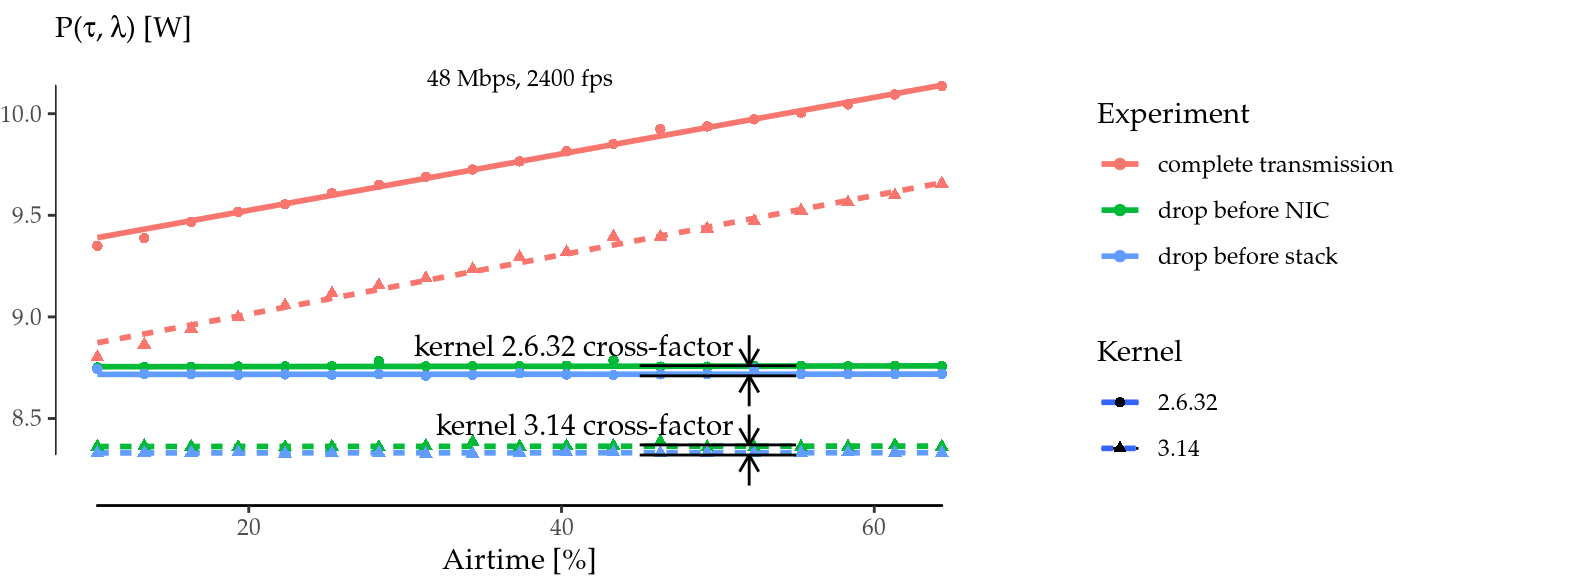
\includegraphics{04-netstacks_files/figure-latex/c1-1} 

}

\caption[Power consumption breakdown vs.~airtime with fixed C1 state for
kernels 2.6.32 and 3.14.]{Power consumption breakdown vs.~airtime with fixed C1 state for
kernels 2.6.32 and 3.14.}\label{fig:c1}
\end{figure*}

Figure \ref{fig:c1} shows the energy breakdown for both kernels, 2.6.32
and 3.14, when only the C1 state is enabled. As can be seen, the
obtained kernel cross-factor is almost negligible, which suggests that
Intel Haswell's C1 state saves a very small amount of power, unlike the
Soekris' C1 state as shown in Figure \ref{fig:validation1}.

There is also a baseline power difference between kernels. This offset
can be ascribed to several factors. For instance, a lot of code has
changed ---and probably improved--- between those kernel versions. In
particular, the scheduler and the \texttt{cpuidle} algorithms have
evolved. Moreover, the compiler used has changed also.

At this respect, we can calculate the complete cross-factor (including
the user-space, as done in Section \ref{validation}) by extracting the
slopes of the regressions of Figure \ref{fig:c1-cfactor}. These values
are comparable to the Linksys case reported by \citet{Serrano2014}:
\(0.51(2)\) mJ (kernel 2.6.32) and \(0.38(2)\) mJ (kernel 3.14).




\begin{figure}

{\centering 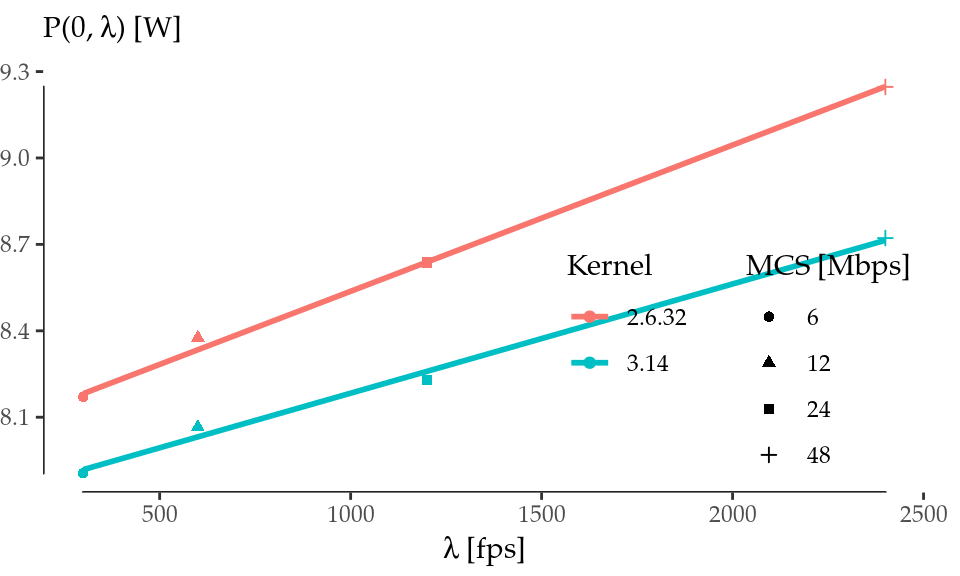
\includegraphics{04-netstacks_files/figure-latex/c1-cfactor-1} 

}

\caption[Power consumption offset (\(\tau=0\)) vs.~framerate
with fixed C1 state for kernels 2.6.32 and 3.14.]{Power consumption offset (\(\tau=0\)) vs.~framerate
with fixed C1 state for kernels 2.6.32 and 3.14.}\label{fig:c1-cfactor}
\end{figure}

It is also important to note that, unlike the results from Figure
\ref{fig:validation1}, there is absolutely no dependence on the frame
size in this case. Our guess is that RAM memory consumption would be
proportional to the frame size and may have a small but still
perceptible impact in low-power devices, but it is negligible compared
to the consumption of a laptop's CPU. As a consequence, the frame size
can be removed as a parameter from the cross-factor analysis in laptops.

\hypertarget{power-consumption-with-full-cpuidle-subsystem}{%
\section{\texorpdfstring{Power Consumption with Full \texttt{cpuidle}
Subsystem}{Power Consumption with Full cpuidle Subsystem}}\label{power-consumption-with-full-cpuidle-subsystem}}

With the knowledge acquired so far, we can move onto a more realistic
scenario by enabling the whole \texttt{cpuidle} subsystem, i.e., keeping
both ACPI C-states enabled and letting the governor decide.




\begin{figure*}

{\centering 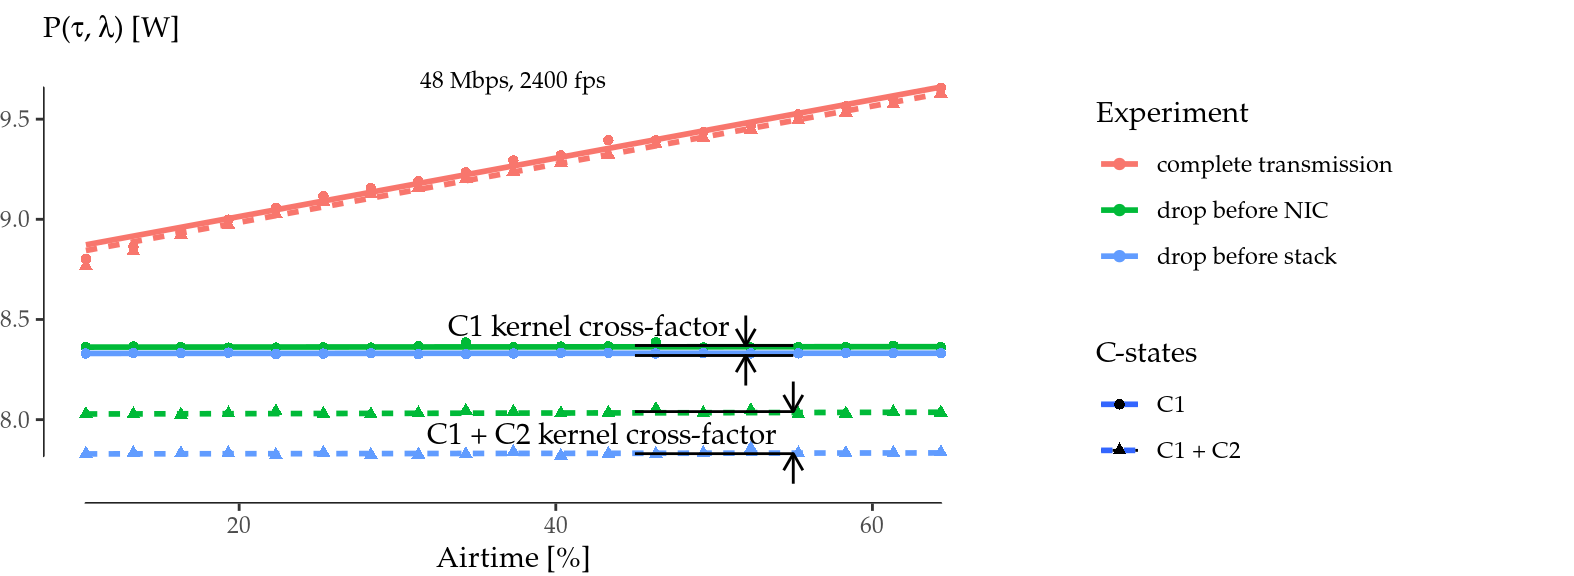
\includegraphics{04-netstacks_files/figure-latex/c12-1} 

}

\caption[Power consumption breakdown vs.~airtime with two
\texttt{cpuidle} configurations for kernel 3.14.]{Power consumption breakdown vs.~airtime with two
\texttt{cpuidle} configurations for kernel 3.14.}\label{fig:c12}
\end{figure*}

Figure \ref{fig:c12} depicts the energy breakdown for kernel 3.14 with
full \texttt{cpuidle} subsystem (C1+C2 enabled) and compares it to the
previous case (C1 only). By enabling C2, the consumption appears to be
always lower up to driver level (blue and green lines). Nevertheless,
the consumption of complete transmissions (red lines) is lower in the
300 fps case (not shown here), but it is the same in the 2400 fps case.




\begin{figure}

{\centering 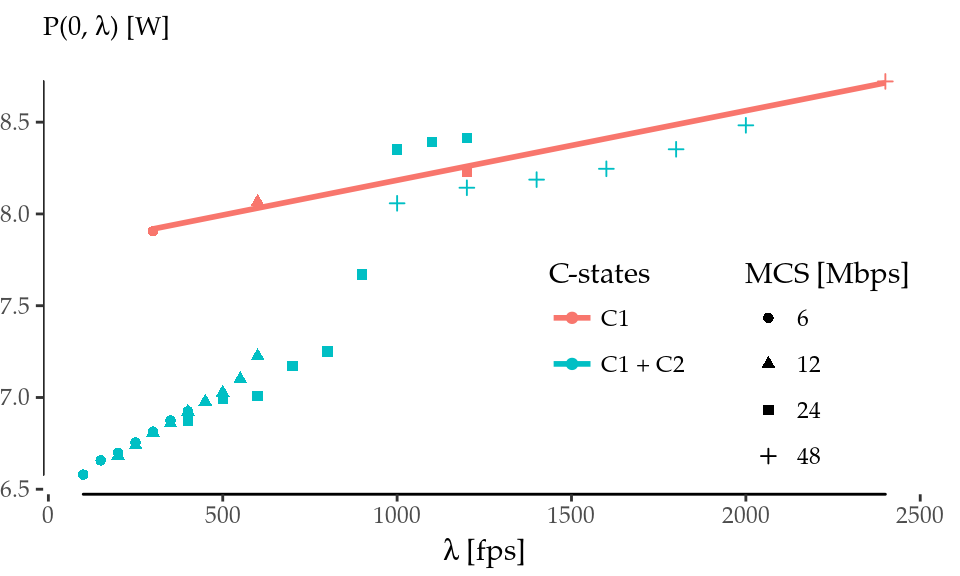
\includegraphics{04-netstacks_files/figure-latex/c12-cfactor-1} 

}

\caption[Power consumption offset (\(\tau=0\)) vs.~framerate
with two \texttt{cpuidle} configurations for kernel 3.14.]{Power consumption offset (\(\tau=0\)) vs.~framerate
with two \texttt{cpuidle} configurations for kernel 3.14.}\label{fig:c12-cfactor}
\end{figure}

Figure \ref{fig:c12-cfactor} compares the offsets of complete
transmissions in Figure \ref{fig:c12} for both cases: C1+C2 and C1 only.
The red line corresponds to C1: as expected, its behaviour is linear as
seen in Figure \ref{fig:c1-cfactor}. On the other hand, the C1+C2 case
(blue points) is not linear globally. It comprises three clearly
distinct parts: when the framerate is low, there is an approximately
linear behaviour because the CPU only uses C2; when the framerate is
high, C2 is no longer used, and the slope matches the red line; between
them, the behaviour becomes unpredictable because of the mix of C1 and
C2. Therefore, the cross-factor as defined by \citet{Serrano2014} makes
no sense anymore. When all the C-states are active, there is no linear
behaviour anymore: we cannot talk neither about a slope nor a fixed
energy toll per frame.

Furthermore, we had assumed, as \citet{Serrano2014}, that we can simply
drop the packets at certain points, measure the mean power up to those
points and represent all this as an energy breakdown. But obviously this
is not true either. For instance, Figure \ref{fig:c12} shows that the
CPU is not entering C2 when complete transmissions are performed, and
the consumption is the same as in the C1-only case. On the other hand,
the CPU is clearly spending some time in C2 when the frames are dropped
earlier. Even it seems that the network stack is consuming more power
because the energy gap (between green and blue lines) is larger.
Evidently, it should be the opposite: the stack would be consuming less
power as soon as it enters a lower C-state.

\hypertarget{exploring-the-cpuidle-subsystem}{%
\section{\texorpdfstring{Exploring the \texttt{cpuidle}
Subsystem}{Exploring the cpuidle Subsystem}}\label{exploring-the-cpuidle-subsystem}}

As stated in previous sections, the \texttt{cpuidle} subsystem is a very
complex component. Kernel timer events are the main input for the
governor algorithm as they often indicate the next wake-up of the CPU,
but the running average used to scale the latter makes it unpredictable,
since it depends on the recent state of the whole machine. The purpose
of this section is to shed some light on the linkage between the
residence time of C-states, the number of wake-ups per second, the CPU
load and the transmission of wireless frames.

We implemented a very simple application\footnote{Available at
  \url{https://github.com/Enchufa2/udperf}} with two modes of operation:
it is capable of setting a kernel timer at a given constant rate and,
when this timer is triggered, it (i) does nothing or (ii) sends a UDP
packet. At the same time, it calculates the mean residence time of each
C-state over the whole execution.

Figures \ref{fig:residency-wakeups} have been compiled using this tool.
The additional CPU load was added on top of the latter using a modified
version of \texttt{lookbusy}\footnote{\url{http://www.devin.com/lookbusy}}.
Figure \ref{fig:power-wakeups} compares the two previous figures in
terms of power consumption.





\begin{figure*}

{\centering 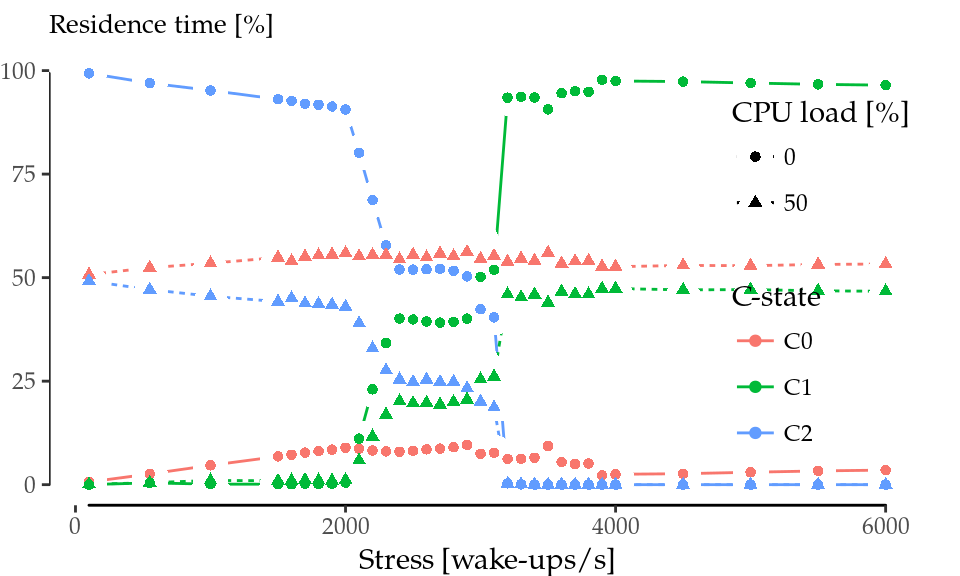
\includegraphics[width=0.49\linewidth]{04-netstacks_files/figure-latex/residency-wakeups-1} 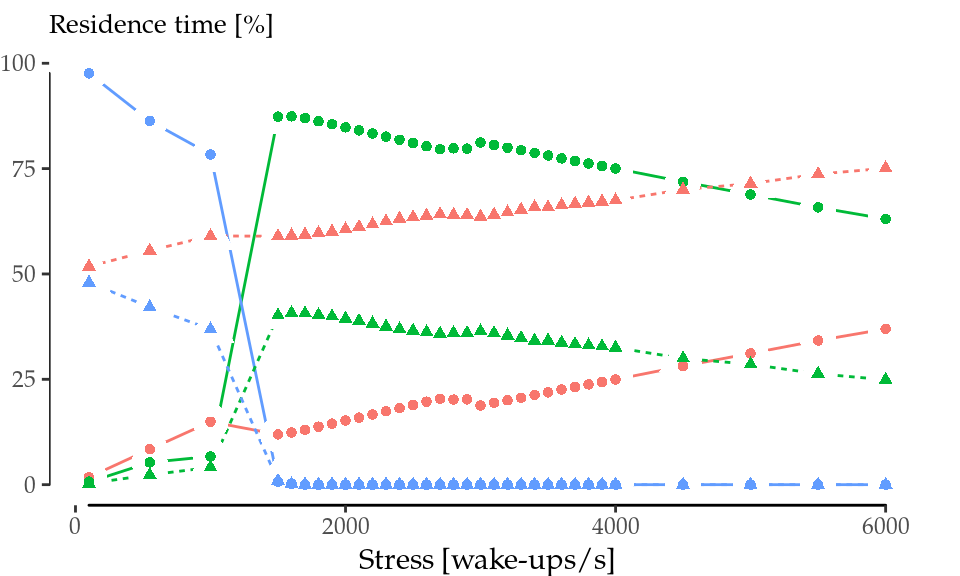
\includegraphics[width=0.49\linewidth]{04-netstacks_files/figure-latex/residency-wakeups-2} 

}

\caption[Residence time of each C-state vs.~wake-ups/s
for kernel 3.14. Each wake-up does nothing (left) or performs a UDP
transmission (right).]{Residence time of each C-state vs.~wake-ups/s
for kernel 3.14. Each wake-up does nothing (left) or performs a UDP
transmission (right).}\label{fig:residency-wakeups}
\end{figure*}




\begin{figure}

{\centering 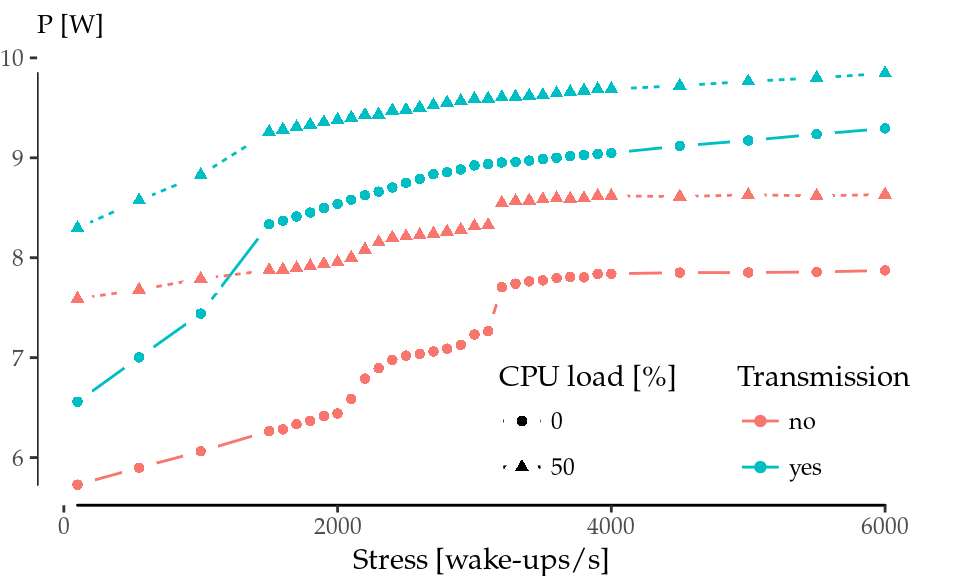
\includegraphics{04-netstacks_files/figure-latex/power-wakeups-1} 

}

\caption[Power consumption offset vs.~wake-ups/s for kernel
3.14.]{Power consumption offset vs.~wake-ups/s for kernel
3.14.}\label{fig:power-wakeups}
\end{figure}

In Figure \ref{fig:residency-wakeups} (left), the only source of
wake-ups is the kernel timer that our tool sets. Each C-state is
represented by a different colour, and shapes and line types distinguish
between CPU loads. The first observation is that the addition of a
substantial source of CPU load has no impact on the distribution of
residence times. Another important observation is that, up to 2000 and
from 3500 wake-ups/s onwards, there is only one active idle state (C2 or
C1 respectively), and the behaviour is linear. This fact can be verified
by checking the power consumption (Figure \ref{fig:power-wakeups}, red
lines). From 2000 to 3500 wake-ups/s, the transition between C-states
occurs in a non-linear way.

In Figure \ref{fig:residency-wakeups} (right), on other hand, there is
another source of wake-ups: hardware interrupts caused by the wireless
card each time a packet is sent. The transition between states occurs
earlier because there is actually twice the number of wake-ups. And,
again, the CPU load shows no impact on the distribution of residence
times.

\newthought{These are partial results} and are limited to constant rate
wake-ups, but these findings are in line with the non-linearities
previously discovered in the cross-factor and they confirms the enormous
complexity we face.

\hypertarget{summary-1}{%
\section{Summary}\label{summary-1}}

This chapter follows the path set out by \citet{Serrano2014} with the
discovery of the cross-factor, an energy toll not accounted by classical
energy models and associated to the very fact that frames are processed
along the network stack. We have introduced the laptop as a more
suitable device to perform whole-device energy measurements in order to
deseed the root causes of the cross-factor by taking advantage of the
wide range of debugging tools that such platform enables.

Our
results\cite[0pt]{contrib-04a,contrib-04b}\marginnote{\hypersetup{hidelinks}\color{white}\citet{contrib-04a,contrib-04b}},
albeit preliminary, provide several fundamental insights on this matter:

\begin{itemize}
\tightlist
\item
  We have identified the CPU as the leading cause of the cross-factor in
  laptops. Thus, the cross-factor shows absolutely no dependence on the
  frame size, because the RAM memory has no significant impact in the
  overall energy consumption of wireless transmissions. On the other
  hand, low-powered devices, like the Soekris, show a very small but
  perceptible dependency that can be ascribed to the RAM memory.
\item
  The CPU's C-state management plays a central role in the energy
  consumption, because a CPU spends most of the time in idle mode.
\item
  When the C-state management subsystem is not present in the OS, the
  device enters C1 in idle mode (halted) and cannot benefit from lower
  idle states.
\item
  In contrast to low-powered devices, the C1 state of a laptop's CPU
  saves a very small amount of power.
\item
  With a fully functional C-state management subsystem, the linear
  behaviour disappears. In consequence, we cannot talk about
  cross-factor as a fixed energy toll per frame.
\item
  A non-linear behaviour implies that we cannot perform energy
  breakdowns by dropping packets inside the transmission chain.
  Therefore, new methodologies and techniques are required to enable
  energy debugging.
\item
  C-state residence times depend primarily on the number of wake-ups per
  second produced by software and hardware interrupts. However, they
  show no dependence on the CPU load.
\end{itemize}

Further research is needed in order to fully understand the key role of
the C-state subsystem in the energy consumption of wireless
communications, as well as to investigate other processor capabilities
not accounted for in this work, such as P-states and multicore support.

\hypertarget{ch:05}{%
\chapter{Leveraging Micro-Sleep Opportunities in 802.11}\label{ch:05}}

\newthought{In this chapter}, we revisit the idea of packet overhearing
as a trigger for sleep opportunities, and we take it one step further to
the range of microseconds. To this end, we experimentally explore the
timing limitations of 802.11 cards. Then, we analyse 802.11 to identify
potential micro-sleep opportunities, taking into account practical
CSMA-related issues (e.g., capture effect, hidden nodes) not considered
in prior work.

Building on this knowledge, we design \(\mu\)Nap, a local
standard-compliant energy-saving mechanism for 802.11 WLANs. With
\(\mu\)Nap, a station is capable of saving energy during packet
overhearing autonomously, with full independence from the 802.11
capabilities supported or other power saving mechanisms in use, which
makes it backwards compatible and incrementally deployable.

Finally, the performance of the algorithm is evaluated based on our
measurements and real wireless traces. In a brief discussion of the
impact and applicability of our mechanism, we draw attention to the need
for standardising hardware capabilities in terms of energy in 802.11.

\hypertarget{state-transition-times}{%
\section{State Transition Times in 802.11
Cards}\label{state-transition-times}}

From the hardware point of view, the standard Power Save (PS) mechanism
requires supporting two states of operation: the \emph{awake state} and
the \emph{sleep state}. The latter is implemented using a secondary
low-frequency clock. Indeed, it is well-known that the power consumption
of digital devices is proportional to the clock
rate\cite[0pt]{Zhang2012}\marginnote{\hypersetup{hidelinks}\color{white}\citet{Zhang2012}}.
In fact, other types of devices, such as microcontroller-based devices
or modern general-purpose CPUs, implement sleep states in the same way.

For any microcontroller-based device with at least an idle state and a
sleep state, one would expect the following behaviour for an ideal
sleep. The device was in idle state, consuming \(P_\mathrm{idle}\),
when, at an instant \(t_\mathrm{off}\), the sleep state is triggered and
the consumption falls to \(P_\mathrm{sleep}\). A secondary low-power
clock decrements a timer of duration
\(\Delta t_\mathrm{sleep} = t_\mathrm{on} - t_\mathrm{off}\), and then
the expiration of this timer triggers the wake-up at \(t_\mathrm{on}\).
The switching between states would be instantaneous and the energy
saving would be
%
\begin{equation}
 E_\mathrm{save} = (P_\mathrm{idle} - P_\mathrm{sleep}) \cdot \Delta t_\mathrm{sleep}
 \label{eq:idealsleep}
\end{equation}
%


This estimate could be considered valid for a time scale in the range of
tens of milliseconds at least, but this is no longer true for
micro-sleeps. Instead, Figure \ref{fig:timing} presents a conceptual
breakdown of a generic micro-sleep.



\begin{figure}

{\centering 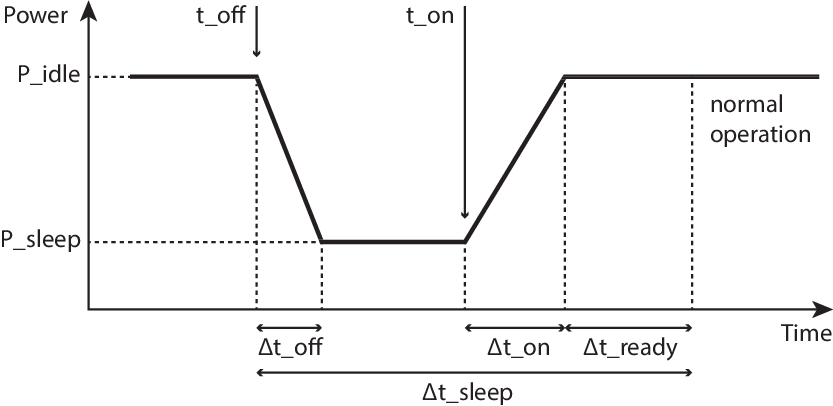
\includegraphics{img/05/timing} 

}

\caption[Generic sleep breakdown.]{Generic sleep breakdown.}\label{fig:timing}
\end{figure}

After the sleep state is triggered at \(t_\mathrm{off}\), it takes
\(\Delta t_\mathrm{off}\) before the power consumption actually reaches
\(P_\mathrm{sleep}\). Similarly, after the wake-up is triggered at
\(t_\mathrm{on}\), it takes some time, \(\Delta t_\mathrm{on}\), to
reach \(P_\mathrm{idle}\). Finally, the circuitry might need some
additional time \(\Delta t_\mathrm{ready}\) to stabilise and operate
normally. Thus, the most general expression for the energy saved in a
micro-sleep is the following:
%
\begin{equation}
\begin{split}
 E'_\mathrm{save} =&~ E_\mathrm{save} - E_\mathrm{waste} \\
 =&~ (P_\mathrm{idle} - P_\mathrm{sleep}) \cdot (\Delta t_\mathrm{sleep} -\Delta t_\mathrm{ready}) \\
 &- \int_{\Delta t_\mathrm{off} \cup \Delta t_\mathrm{on}} (P - P_\mathrm{sleep}) \cdot dt
\end{split}
\label{eq:realsleep}
\end{equation}
%
where we have considered a general waveform \(P(t)\) for the transients
\(\Delta t_\mathrm{off}\) and \(\Delta t_\mathrm{on}\).
\(E_\mathrm{waste}\) represents an energy toll per sleep when compared
to the ideal case.

\newthought{Our next objective} is to quantify these limiting
parameters, which can be defined as follows:

\begin{description}
\tightlist
\item[\(\Delta t_\mathrm{off}\)]
is the time required to switch from idle power and to sleep power
consumption.
\item[\(\Delta t_\mathrm{on}\)]
is the time required to switch from sleep power to idle power
consumption.
\item[\(\Delta t_\mathrm{ready}\)]
is the time required for the electronics to stabilise and become ready
to transmit/receive.
\end{description}

The sum of this set of parameters defines the minimum sleep time,
\(\Delta t_\mathrm{sleep,min}\), for a given device:
%
\begin{equation}
 \Delta t_\mathrm{sleep,min} = \Delta t_\mathrm{off} + \Delta t_\mathrm{on} + \Delta t_\mathrm{ready}
 \label{eq:sleepmin}
\end{equation}
%


Performing this experimental characterisation requires the ability to
timely trigger the sleep mode on demand. As stated in Section
\ref{anatomy-of-a-laptop-computer}, most COTS cards are not suitable for
this task, because they implement all the low-level operations in an
internal proprietary binary firmware. However, those cards based on the
open-source driver \texttt{ath9k}, like the one presented in previous
chapters\footnote{Atheros AR9280.} are well suited for our needs. The
driver has access to very low level functionality (e.g., supporting
triggering the sleep mode by just writing into a register).

\newthought{This characterisation} follows the setup depicted in Section
\ref{per-component-measurements}, Figure \ref{fig:testbed-card}. The
card under test is associated to an access point (AP) in 11a mode to
avoid any interfering traffic from neighbouring networks. This AP is
placed very close to the node to obtain the best possible signal
quality, as we are simply interested in not losing the connectivity for
this experiment. With this setup, the idea is to trigger the sleep
state, then bring the interface back to idle and finally trigger the
transmission of a buffered packet as fast as possible, in order to find
the timing constraints imposed by the hardware in the power signature.
From an initial stable power level, with the interface associated and in
idle mode, we would expect a falling edge to a lower power level
corresponding to the sleep state. Then the power level would raise again
to the idle level and, finally, a big power peak would mark the
transmission of the packet. By correlating the timestamps of our
commands and the timestamps of the measured power signature, we will be
able to measure the limiting parameters
\(\Delta t_\mathrm{off}, \Delta t_\mathrm{on}, \Delta t_\mathrm{ready}\).

The methodology to reproduce these steps required hacking the
\texttt{ath9k} driver to timely trigger write operations in the proper
card registers, and to induce a transmission of a pre-buffered packet
directly in the device without going through the entire network stack. A
simple hack in the \texttt{ath9k} module\footnote{Available at
  \url{https://github.com/Enchufa2/crap/tree/master/ath9k/downup}.}
allows us to perform the following experiment:

\begin{enumerate}
\def\labelenumi{\arabic{enumi}.}
\setcounter{enumi}{-1}
\tightlist
\item
  Initially, the card is in idle state, connected to the AP.
\item
  A RAW socket (Linux \texttt{AF\_PACKET} socket) is created and a
  socket buffer is prepared with a fake packet.
\item
  \(t_\mathrm{off}\) is triggered by writing a register in the card,
  which has proved to be almost instantaneous in kernel space.
\item
  A micro-delay of 60 \(\mu\)s is introduced in order to give the card
  time to react.
\item
  \(t_\mathrm{on}\) is triggered with another register write.
\item
  Another timer sets a programmable delay.
\item
  The fake frame is sent using a low-level interface, i.e., calling the
  function \texttt{ndo\_start\_xmit()} from the \texttt{net\_device}
  operations directly. By doing this, we try to spend very little time
  in kernel.
\end{enumerate}

The power signature recorded as a result of this experiment is shown in
Figure \ref{fig:sleep-tx} (left).



\begin{figure*}

{\centering 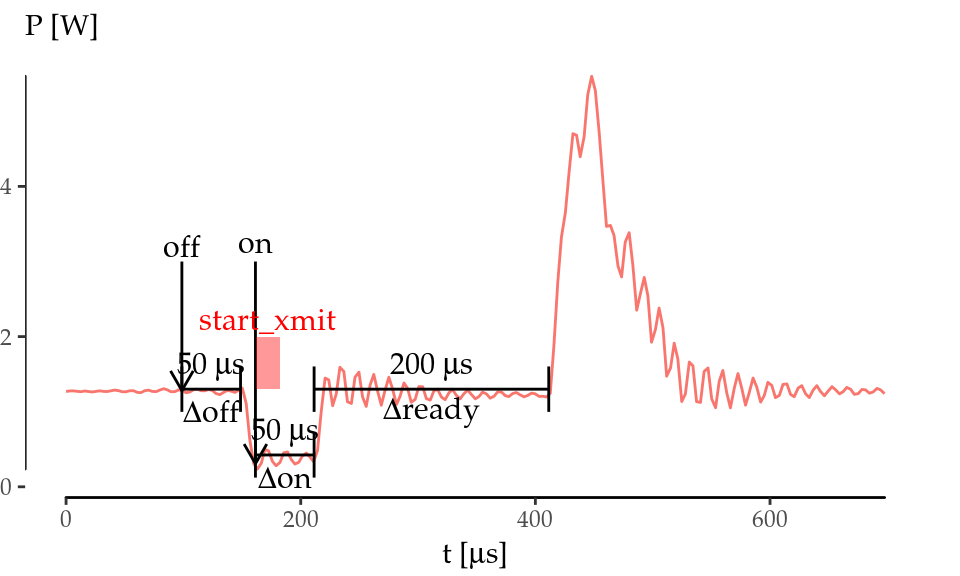
\includegraphics[width=0.49\linewidth]{05-unap_files/figure-latex/sleep-tx-1} 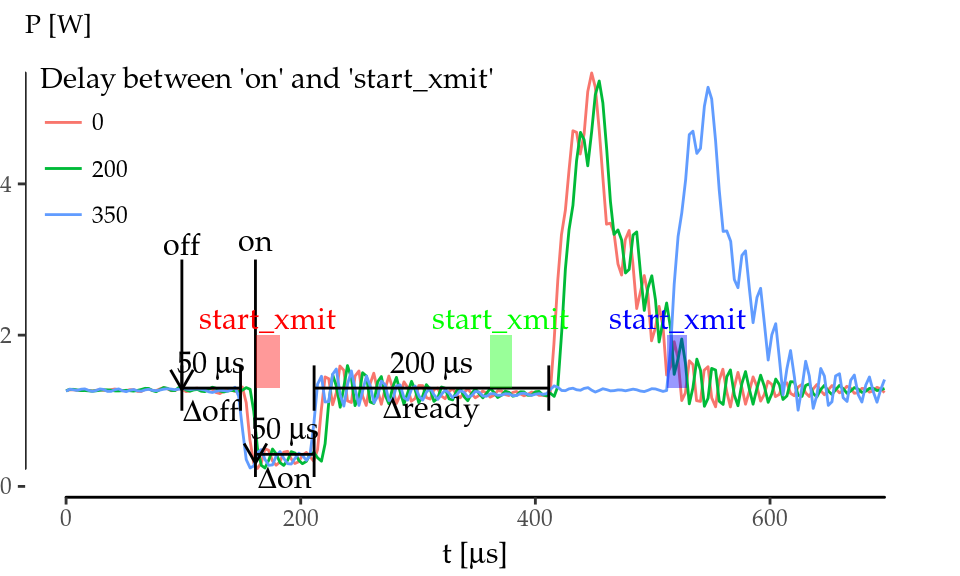
\includegraphics[width=0.49\linewidth]{05-unap_files/figure-latex/sleep-tx-2} 

}

\caption[Atheros AR9280 timing characterisation.]{Atheros AR9280 timing characterisation.}\label{fig:sleep-tx}
\end{figure*}

As we can see, the card spends \(\Delta t_\mathrm{off} = 50\) \(\mu\)s
consuming \(P_\mathrm{idle}\) and then it switches off to
\(P_\mathrm{sleep}\) in only 10 \(\mu\)s. Then, \(t_\mathrm{on}\) is
triggered. Similarly, the card spends \(\Delta t_\mathrm{on} = 50\)
\(\mu\)s consuming \(P_\mathrm{sleep}\) and it wakes up almost
instantaneously. Note that the transmission of the packet is triggered
right after the \(t_\mathrm{on}\) event and the frame spends very little
time at the kernel (the time spent in kernel corresponds to the width of
the rectangle labelled as \texttt{start\_xmit} in the graph).
Nonetheless, the card sends the packet 200 \(\mu\)s after returning to
idle, even though the frame was ready for transmission much earlier.

To understand the reasons for the delay in the frame transmission
observed above, we performed an experiment in which frame transmissions
were triggered at different points in time by introducing different
delays between the \(t_\mathrm{on}\) and \texttt{start\_xmit} events.
Figure \ref{fig:sleep-tx} (right) shows that the card starts
transmitting always in the same instant whenever the kernel triggers the
transmission within the first 250 \(\mu\)s right after the
\(t_\mathrm{on}\) event (lines 0 and 200). Otherwise, the card starts
transmitting almost instantaneously (line 350). This experiments
demonstrate that the device needs \(\Delta t_\mathrm{ready} = 200\)
\(\mu\)s to get ready to transmit/receive after returning to idle.

\newthought{Summing up}, our experiments show that, if we want to bring
this card to sleep during a certain time \(\Delta t_\mathrm{sleep}\), we
should take into account that it requires a minimum sleep time
\(\Delta t_\mathrm{sleep,min}=300\) \(\mu\)s. Therefore,
\(\Delta t_\mathrm{sleep} \geq \Delta t_\mathrm{sleep,min}\) must be
satisfied, and we must program the \(t_\mathrm{on}\) interrupt to be
triggered \(\Delta t_\mathrm{on} + \Delta t_\mathrm{ready}=250\)
\(\mu\)s before the end of the sleep. Note also that the card wastes a
fixed time \(\Delta t_\mathrm{waste}\) consuming \(P_\mathrm{idle}\):
%
\begin{equation}
 \Delta t_\mathrm{waste} = \Delta t_\mathrm{off} + \Delta t_\mathrm{ready}
 \label{eq:twaste}
\end{equation}
%
which is equal to 250 \(\mu\)s also. Thus, the total time in sleep state
is \(\Delta t_\mathrm{sleep} - \Delta t_\mathrm{waste}\), and the energy
toll from Equation \eqref{eq:realsleep} can be simplified as follows:
%
\begin{equation}
 E_\mathrm{waste} \approx (P_\mathrm{idle} - P_\mathrm{sleep})\cdot\Delta t_\mathrm{waste}
 \label{eq:Ewaste}
\end{equation}
%
\hypertarget{protocol-analysis-and-practical-issues}{%
\section{Protocol Analysis and Practical
Issues}\label{protocol-analysis-and-practical-issues}}

The key idea of this chapter is to put the interface to sleep during
packet overhearing while meeting the constraint
\(\Delta t_\mathrm{sleep,min}\) identified in the previous section.
Additionally, such a mechanism should be local in order to be
incrementally deployable, standard-compliant, and should take into
account real-world practical issues. For this purpose, we first identify
potential micro-sleep opportunities in 802.11, and explore well-known
practical issues of WLAN networks that had not been addressed by
previous energy-saving schemes.

\hypertarget{identifying-potential-micro-sleep-opportunities}{%
\subsection{Identifying Potential Micro-Sleep
Opportunities}\label{identifying-potential-micro-sleep-opportunities}}

Due to the CSMA mechanism, an 802.11 station (STA) receives every single
frame from its Service Set Identifier (SSID) or from others in the same
channel (even some frames from overlapping channels). Upon receiving a
frame, a STA checks the Frame Check Sequence (FCS) for errors and then,
and only after having received the entire frame, it discards the frame
if it is not the recipient. In 802.11 terminology, this is called
\emph{packet overhearing}. Since packet overhearing consumes the power
corresponding to a full packet reception that is not intended for the
station, it represents a source of inefficiency. Thus, we could avoid
this unnecessary power consumption by triggering micro-sleeps that bring
the wireless card to a low-energy state.

Indeed, the Physical Layer Convergence Procedure (PLCP) carries the
necessary information (rate and length) to know the duration of the PLCP
Service Data Unit (PSDU), which consists of a MAC frame or an aggregate
of frames. And the first 10 bytes of a MAC frame indicate the intended
receiver, so a frame could be discarded very early, and the station
could be brought to sleep if the hardware allows for such a short
sleeping time. Therefore, the most naive micro-sleep mechanism could
determine, given the constraint \(\Delta t_\mathrm{sleep,min}\), whether
the interface could be switched off in a frame-by-frame basis. And
additionally, this behaviour can be further improved by leveraging the
802.11 virtual carrier-sensing mechanism.

Virtual carrier-sensing allows STAs not only to seize the channel for a
single transmission, but also to signal a longer exchange with another
STA. For instance, this exchange can include the acknowledgement sent by
the receiver, or multiple frames from a station in a single transmission
opportunity (TXOP). MAC frames carry a duration value that updates the
Network Allocation Vector (NAV), which is a counter indicating how much
time the channel will be busy due to the exchange of frames triggered by
the current frame. This duration field is, for our benefit, enclosed in
the first 10 bytes of the MAC header too. Therefore, the NAV could be
exploited to obtain substantial gains in terms of energy.

\newthought{In order to unveil} potential sleeping opportunities within
the different states of operation in 802.11, first of all we review the
setting of the NAV. 802.11 comprises two families of channel access
methods. Within the legacy methods, the Distributed Coordination
Function (DCF) is the basic mechanism with which all STAs contend
employing CMSA/CA with binary exponential backoff. In this scheme, the
duration value provides single protection: the setting of the NAV value
is such that protects up to the end of one frame (data, management) plus
any additional overhead (control frames)\footnote{For instance, this
  could be the ACK following a data frame or the CTS + data + ACK
  following an RTS.}.

When the Point Coordination Function (PCF) is used, time between beacons
is rigidly divided into contention and contention-free periods (CP and
CFP, respectively). The AP starts the CFP by setting the duration value
in the beacon to its maximum value\footnote{Which is 32 768; see
  \citet[Table 8-3]{80211} for further details about the duration/ID
  field encoding}. Then, it coordinates the communication by sending
CF-Poll frames to each STA. As a consequence, a STA cannot use the NAV
to sleep during the CFP, because it must remain CF-pollable, but it
still can doze during each individual packet transmission. In the CP,
DCF is used.

802.11e introduces traffic categories (TC), the concept of TXOP, and a
new family of access methods called Hybrid Coordination Function (HCF),
which includes the Enhanced Distributed Channel Access (EDCA) and the
HCF Controlled Channel Access (HCCA). These two methods are the
QoS-aware versions of DCF and PCF respectively.

Under EDCA, there are two classes of duration values: single protection,
as in DCF, and multiple protection, where the NAV protects up to the end
of a sequence of frames within the same TXOP. By setting the appropriate
TC, any STA may start a TXOP, which is zero for background and
best-effort traffic, and of several milliseconds for video and audio
traffic as defined in the standard\footnote{See \citet[Table
  8-105]{80211}.}. A non-zero TXOP may be used for dozing, as 11ac does,
but these are long sleeps and the AP needs to support this feature,
because a TXOP may be truncated at any moment with a CF-End frame, and
it must keep buffering any frame directed to any 11ac dozing STA until
the NAV set at the start of the TXOP has expired.

HCCA works similarly to PCF, but under HCCA, the CFP can be started at
almost any time. In the CFP, when the AP sends a CF-poll to a STA, it
sets the NAV of other STAs for an amount equal to the TXOP.
Nevertheless, the AP may reclaim the TXOP if it ends too early (e.g.,
the STA has nothing to transmit) by resetting the NAV of other STAs with
another CF-Poll. Again, the NAV cannot be locally exploited to perform
energy saving during a CFP.

Finally, there is another special case in which the NAV cannot be
exploited either. 802.11g was designed to bring the advantages of 11a to
the 2.4 GHz band. In order to interoperate with older 11b deployments,
it introduces CTS-to-self frames (also used by more recent amendments
such as 11n and 11ac). These are standard CTS frames, transmitted at a
legacy rate and not preceded by an RTS, that are sent by a certain STA
to itself to seize the channel before sending a data frame. In this
case, the other STAs cannot know which will be the destination of the
next frame. Therefore, they should not use the duration field of a CTS
for dozing.

\hypertarget{impact-of-capture-effect}{%
\subsection{Impact of Capture Effect}\label{impact-of-capture-effect}}

It is well-known that a high-power transmission can totally blind
another one with a lower SNR. Theoretically, two STAs seizing the
channel at the same time yields a collision. However, in practice, if
the power ratio is sufficiently high, a wireless card is able to decode
the high-power frame without error, thus ignoring the other
transmission. This is called \emph{capture effect}, and although not
described by the standard, it must be taken into account as it is
present in real deployments.

According to \citet{Lee2007}\cite{Lee2007}, there are two types of
capture effect depending on the order of the frames: if the high-power
frame comes first, it is called \emph{first} capture effect; otherwise,
it is called \emph{second} capture effect. The first one is equivalent
to receiving a frame and some noise after it, and then it has no impact
in our analysis. In the second capture effect, the receiving STA stops
decoding the PLCP of the low-power frame and switches to another with
higher power. If the latter arrives \emph{before} a power-saving
mechanism makes the decision to go to sleep, the mechanism introduces no
misbehaviour.

However, \citet{Lee2007} suggests that a high-power transmission could
blind a low-power one \emph{at any time}, even when the actual data
transmission has begun. This is called \emph{Message in Message} (MIM)
in the
literature\cite[0pt]{mim1,mim2}\marginnote{\hypersetup{hidelinks}\color{white}\citet{mim1,mim2}},
and it could negatively impact the performance of an interface
implementing an energy-efficiency mechanism based on packet overhearing.
In the following, we will provide new experimental evidence supporting
that this issue still holds in modern wireless cards.

\newthought{We evaluated} the properties of the MIM effect with an
experimental setup consisting of a card under test, a brand new 802.11ac
three-stream Qualcomm Atheros QCA988x card, and three additional helper
nodes. These are equipped with Broadcom KBFG4318 802.11g cards, whose
behaviour can be changed with the open-source firmware
OpenFWWF\cite[0pt]{openfwwfweb}\marginnote{\hypersetup{hidelinks}\color{white}\citet{openfwwfweb}}.
We disable the carrier sensing and back-off mechanisms so that we can
decide the departure time of every transmitted frame with 1 \(\mu\)s
granularity with respect to the internal 1MHz clock.



\begin{marginfigure}

{\centering 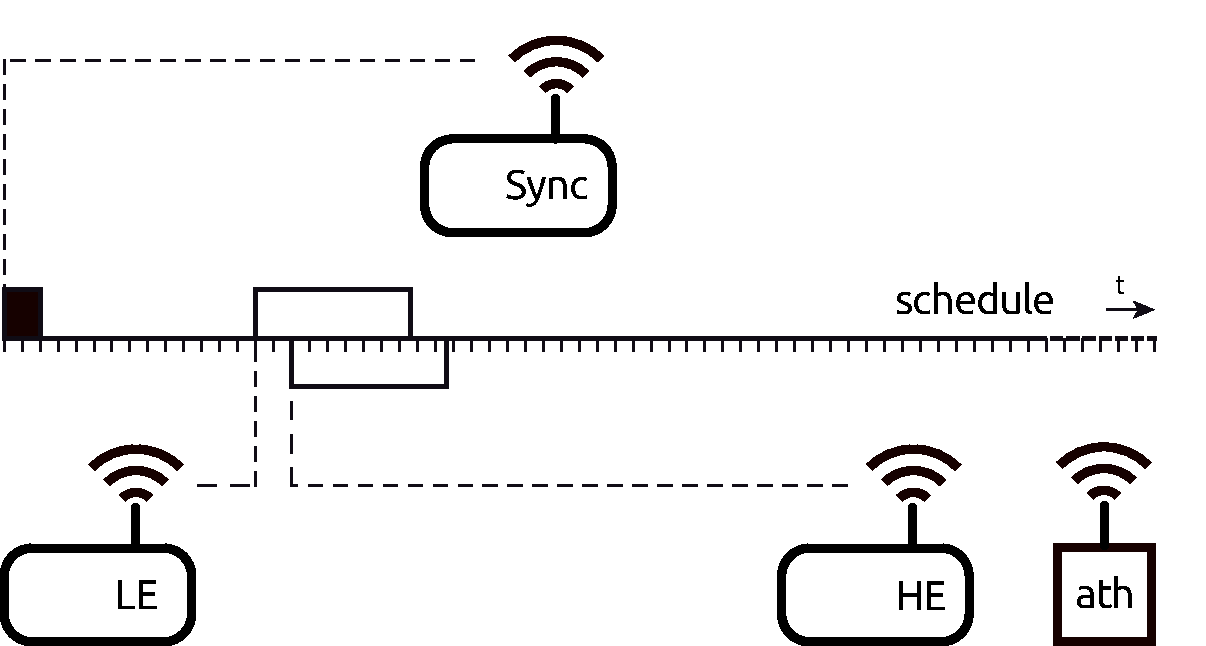
\includegraphics[width=1\linewidth]{img/05/testbed-francesco} 

}

\caption[Measurement setup for the MIM effect.]{Measurement setup for the MIM effect.}\label{fig:secondcapture}
\end{marginfigure}

Figure \ref{fig:secondcapture} depicts the measurement setup, which
consists of a node equipped with our Atheros card under test
(\emph{ath}), a synchronization (Sync) node, a \emph{high energy} (HE)
node and a \emph{low energy} (LE) node. These two HE and LE nodes were
manually carried around at different distances with respect to the
\emph{ath} node until we reached the desired power levels.

The Sync node transmits 80-byte long beacon-like frames periodically at
48 Mbps, one beacon every 8192 \(\mu\)s: the time among consecutive
beacons is divided in 8 schedules of 1024 \(\mu\)s. Inside each
schedule, time is additionally divided into 64 micro-slots of 16
\(\mu\)s. We then program the firmware of the HE and LE nodes to use the
beacon-like frames for keeping their clocks synchronised and to transmit
a single frame (138-\(\mu\)s long) per schedule starting at a specific
micro-slot. This allows us to always start the transmission of the
\emph{low energy} frame from the LE node before the \emph{high energy}
frame from the HE node, and to configure the exact delay \(\Delta t\) as
a multiple of the micro-slot duration.

For instance, we set up a \(\Delta t = 32\) \(\mu\)s by configuring LE
node to transmit at slot 15, HE node at slot 17. By moving LE node away
from the \emph{ath} node while the HE node is always close, we are able
to control the relative power difference \(\Delta P\) received by the
\emph{ath} node between frames coming from the LE and HE nodes. With the
configured timings, we are able to replicate the reception experiment at
the \emph{ath} node approximately 976 times per second, thus collecting
meaningful statistics in seconds.

\begin{table}

\begin{center}
\begin{tabular}{crrrrr}
\toprule
\multicolumn{2}{c}{ } & \multicolumn{2}{c}{LE frames} & \multicolumn{2}{c}{HE frames} \\
\cmidrule(l{2pt}r{2pt}){3-4} \cmidrule(l{2pt}r{2pt}){5-6}
$\Delta P$ [dB] & $\Delta t$ [$\mu$s] & $\%$ rx & $\%$ err & $\%$ rx & $\%$ err\\
\midrule
 & 0 & 0.04 & 50.00 & 92.00 & 17.67\\

 & 16 & 0.40 & 0.00 & 2.15 & 0.00\\

 & 32 & 99.32 & 99.96 & 0.24 & 0.00\\

 & $\geq$ 48 & 99.10 & 99.75 & 0.34 & 0.00\\

\multirow{-5}{*}{\centering\arraybackslash $\leq$ 5} & $\geq$ 144 & 98.94 & 0.00 & 97.32 & 0.00\\
\cmidrule{1-6}
 & 0 & 0.18 & 0.00 & 99.37 & 0.00\\

 & 16 & 0.37 & 1.11 & 91.87 & 0.00\\

 & 32 & 0.39 & 78.95 & 89.89 & 0.00\\

 & 48 & 1.54 & 68.00 & 95.58 & 0.00\\

 & 64 & 3.22 & 98.73 & 89.83 & 0.00\\

 & 128 & 60.35 & 99.96 & 39.24 & 0.00\\

\multirow{-7}{*}{\centering\arraybackslash $\geq$ 35} & $\geq$ 144 & 95.33 & 0.00 & 99.64 & 0.00\\
\bottomrule
\end{tabular}
\end{center}
\caption{\label{tab:secondcapturet}Message-in-message effect.}
\end{table}

\newthought{We obtained} the results shown in Table
\ref{tab:secondcapturet}. When the energy gap is small (\(\le\) 5 dB),
the MIM effect never enters into play as we can see from the first part
of Table \ref{tab:secondcapturet}. If the two frames are transmitted at
the same time, then the QCA card receives the majority of the HE frames
(92\%) despite some of them are broken (17\%); almost no LE frames are
received. By increasing the delay to 16 \(\mu\)s, the QCA card stops
working: the short delay means that the HE frame collide with the LE one
at the PLCP level. The energy gap does not allow the QCA correlator to
restart decoding a new PLCP and, in fact, only a few frames are
sporadically received. Further increasing the delay allows the QCA card
to correctly receive the PLCP preamble of the LE frame, but then the PDU
decoding is affected by errors (e.g., delay set to 48 \(\mu\)s) because
of collision. Finally, if the delay is high enough so that both frames
fit into a schedule, the QCA card receives everything correctly (\(\ge\)
144 \(\mu\)s).

When the energy gap exceeds a threshold (i.e., more than 35 dB), then
the behaviour of the QCA card changes radically as we can see from the
second part of Table \ref{tab:secondcapturet}: first, with no delay, all
high energy frames are received (expected given that they overkill the
others); second, when both frame types fit in the schedule, all of them
are received, which confirms that the link between LE node and the QCA
is still very good. But, unlike the previous case, HE frames are
received regardless of the delay, which means that the correlator
restarts decoding the PLCP of the second frame because of the higher
energy, enough for distinguishing it from the first frame that simply
turns into a negligible noise.

Thus, our experiments confirm that the MIM effect actually affects
modern wireless cards, and therefore it should be taken into account in
any micro-sleep strategy. Let us consider, for instance, a common
infrastructure-based scenario in which certain STA receives low-power
frames from a distant network in the same channel. If the AP does not
see them, we are facing the hidden node problem. It is clear that none
of these frames will be addressed to our STA, but, if it goes to sleep
during these transmissions, it may lose potential high-power frames from
its BSSID. Therefore, if we perform micro-sleeps under hidden node
conditions, in some cases we may lose frames that we would receive
otherwise thanks to the capture effect. The same situation may happen
within the local BSSID (the low-power frames belong to the same
network), but this is far more rare, as such a hidden node will become
disconnected sooner or later.

\newthought{In order to circumvent} these issues, a STA should only
exploit micro-sleep opportunities arising from its own network. To
discard packets originating from other networks, the algorithm looks at
the BSSID in the receiver address within frames addressed to an AP. If
the frame was sent by an AP, it only needs to read 6 additional bytes
(in the worst case), which are included in the transmitter address. Even
so, these additional bytes do not necessarily involve consuming more
time, depending on the modulation. For instance, for OFDM 11ag rates,
this leads to a time increase of 8 \(\mu\)s at 6 and 9 Mbps, 4 \(\mu\)s
at 12, 18 and 36 Mbps, and no time increase at 24, 48 and 54 Mbps.

\hypertarget{impact-of-errors-in-the-mac-header}{%
\subsection{Impact of Errors in the MAC
Header}\label{impact-of-errors-in-the-mac-header}}

Taking decisions without checking the FCS (placed at the end of the
frame) for errors or adding any protection mechanism may lead to
performance degradation due to frame loss. This problem was firstly
identified by \citet{Balaji2010}\cite{Balaji2010} and
\citet{Prasad2014}\cite{Prasad2014} which, based on purely qualitative
criteria, reached opposite conclusions. The first work advocates for the
need for a new CRC to protect the header bits while the latter dismisses
this need. This section is devoted to analyse quantitatively the impact
of errors.

\newthought{At a first stage}, we need to identify, field by field,
which cases are capable of harming the performance of our algorithm due
to frame loss. The duration/ID field (2 bytes) and the MAC addresses (6
bytes each) are an integral part of our algorithm. According to its
encoding, the duration/ID field will be interpreted as an actual
duration \emph{if and only if the bit 15 is equal to 0}. Given that the
bit 15 is the most significant one, this condition is equivalent to the
value being smaller than 32 768. Therefore, we can distinguish the
following cases in terms of the possible errors:

\begin{itemize}
\tightlist
\item
  \emph{An error changes the bit 15 from 0 to 1}. The field will not be
  interpreted as a duration and hence we will not go to sleep. We will
  be missing an opportunity to save energy, but there will be no frame
  loss and, therefore, the network performance will not be affected.
\item
  \emph{An error changes the bit 15 from 1 to 0}. The field will be
  wrongly interpreted as a duration. The resulting \emph{sleep} will be
  up to 33 ms longer than required, with the potential frame loss
  associated.
\item
  \emph{With the bit 15 equal to 0, an error affects the previous bits}.
  The resulting \emph{sleep} will be shorter or longer that the real
  one. In the first case, we will be missing an opportunity to save
  energy; in the second case, there is again a potential frame loss.
\end{itemize}

Regarding the receiver address field, there exist the following
potential issues:

\begin{itemize}
\tightlist
\item
  \emph{A multicast address changes but remains multicast}. The frame
  will be received and discarded, i.e., the behaviour will be the same
  as with no error. Hence, it does not affect.
\item
  \emph{A unicast address changes to multicast}. The frame will be
  received and discarded after detecting the error. If the unicast frame
  was addressed to this host, it does not affect. If it was addressed to
  another host, we will be missing an opportunity to save energy.
\item
  \emph{A multicast address changes to unicast}. If the unicast frame is
  addressed to this host, it does not affect. If it is addressed to
  another host, we will save energy with a frame which would be
  otherwise received and discarded.
\item
  \emph{Another host's unicast address changes to your own}. This case
  is very unlikely. The frame will be received and discarded, so we will
  be missing an opportunity to save energy.
\item
  \emph{Your own unicast address changes to another's}. We will save
  energy with a frame otherwise received and discarded.
\end{itemize}

As for the transmission address field, this is checked as an additional
protection against the undesirable effects of the already discussed
intra-frame capture effect. If the local BSSID in a packet changes to
another BSSID, we will be missing an opportunity to save energy. It is
extremely unlikely that an error in this field could lead to frame loss:
a frame from a foreign node (belonging to another BSSID and hidden to
our AP) should contain an error that matches the local BSSID in the
precise moment in which our AP tries to send us a frame\footnote{Note
  that this frame might be received because of the MIM effect explained
  previously.}.

Henceforth, we draw the following conclusions:

\begin{itemize}
\tightlist
\item
  Errors at the MAC addresses \emph{do not produce frame loss}, because
  under no circumstances they imply frame loss. The only impact is that
  there will be several new opportunities to save energy and several
  others will be wasted.
\item
  Errors at the duration/ID field, however, \emph{may produce frame
  loss} due to frame loss in periods of time up to 33 ms. Also several
  energy-saving opportunities may be missed without yielding any frame
  loss.
\item
  An error burst affecting both the duration/ID field and the receiver
  address may potentially change the latter in a way that the frame
  would be received (multicast bit set to 1) and discarded, and thus
  preventing the frame loss.
\end{itemize}

\newthought{From the above}, we have that the only case that may yield
performance degradation in terms of frame loss is when we have errors in
the duration/ID field. In the following, we are going to analytically
study and quantify the probability of frame loss in this case. For our
analysis, we first consider statistically independent single-bit errors.
Each bit is considered the outcome of a Bernoulli trial with a success
probability equal to the bit error probability \(p_{b}\). Thus, the
number of bit errors, \(X\), in certain field is given by a Binomial
distribution \(X\sim \operatorname{B}(N, p_b)\), where \(N\) is the
length of that field.

With these assumptions, we can compute the probability of having more
than one erroneous bit, \(\Pr(X \geq 2)\), which is three-four orders of
magnitude smaller than \(p_b\) with realistic \(p_b\) values. Therefore,
we assume that we never have more than one bit error in the frame
header, so the probability of receiving an erroneous duration value with
a single-bit error, \(p_{e,b}\), is the following:
%
\begin{equation}
 p_{e,b} \approx 1 - (1 - p_b)^{15} \label{eq:peb}
\end{equation}
%


However, not all the errors imply a duration value greater than the
original one, but only those which convert a zero into a one. Let us
call \(\operatorname{Hw}(i)\) the Hamming weight, i.e., the number of
ones in the binary representation of the integer \(i\). The probability
of an erroneous duration value greater than the original, \(p_{eg,b}\),
is the following:
%
\begin{equation}
 p_{eg,b}(i) = p_{e,b}\cdot \frac{15 -\operatorname{Hw}(i)}{15}
 \label{eq:pegb}
\end{equation}
%
which represents a fraction of the probability \(p_{e,b}\) and depends
on the original duration \(i\) (before the error).

In order to understand the implications of the above analysis in real
networks, we have analysed the SIGCOMM'08 data
set\cite[0pt]{umd-sigcomm2008-2009-03-02}\marginnote{\hypersetup{hidelinks}\color{white}\citet{umd-sigcomm2008-2009-03-02}}
and gathered which duration values are the most common. In the light of
the results depicted in Table \ref{tab:duration}, it seems reasonable to
approximate \(p_{eg,b}/p_{e,b} \approx 1\), because it is very likely
that the resulting duration will be greater than the original.

\begin{table}

\begin{center}
\begin{tabular}{rrrl}
\toprule
Duration & $\%$ & $p_{eg,b}/p_b$ & Cause\\
\midrule
44 & 62.17 & 0.88 & SIFS + ACK at 24 Mbps\\
0 & 25.23 & 1.00 & Broadcast, multicast frames\\
60 & 6.54 & 0.73 & SIFS + ACK at 6 Mbps\\
48 & 5.82 & 0.87 & SIFS + ACK at 12 Mbps\\
\bottomrule
\end{tabular}
\end{center}
\caption{\label{tab:duration}Most frequent duration values.}
\end{table}

Finally, we can approximate \(p_b\) by the BER and, based on the above
data and considerations, the frame loss probability,
\(p_{\mathrm{loss}}\), due to an excessive sleep interval using a
single-bit error model is the following:
%
\begin{equation}
 p_{\mathrm{loss}} = p_{eg,b} \approx p_{e,b} \approx 1 - (1 - \mathrm{BER})^{15}
 \label{eq:plossbit}
\end{equation}
%


\newthought{This analysis assumes} independent errors. However, it is
well known that errors typically occur in bursts. In order to understand
the impact of error bursts in our scheme, we analyse a scenario with
independent error bursts of length \(X\) bits, where \(X\) is a random
variable. To this end, we use the Neyman-A contagious
model\cite[-10mm]{neyman1939new}\marginnote{\hypersetup{hidelinks}\color{white}\citet{neyman1939new}},
which has been successfully applied in telecommunications to describe
burst error distributions\footnote{E.g., by \citet{s614},
  \citet{becam1985validite} and \citet{irvin1991monitoring}.}. This
model assumes that both the bursts and the burst length are
Poisson-distributed. Although assuming independency between errors in
the same burst may not be accurate, it has been shown that the Neyman-A
model performs well for short
intervals\cite[0pt]{cornaglia1996letter}\marginnote{\hypersetup{hidelinks}\color{white}\citet{cornaglia1996letter}},
which is our case.

The probability of having \(k\) errors in an interval of \(N\) bits,
given the Neyman-A model, is the following:
%
\begin{equation}
 p_N(k) = \frac{\lambda_b^k}{k!}e^{-\lambda_B}\sum_{i=0}^\infty\frac{i^k}{i!}\lambda_B^i e^{-i\lambda_b}
 \label{eq:pNk}
\end{equation}
%
where

\begin{description}
\tightlist
\item[\(\lambda_b\)]
is the average number of bits in a burst.
\item[\(\lambda_B\)]
\(= Np_b/\lambda_b\) is the average number of bursts.
\end{description}

This can be transformed into a recursive formula with finite sums:
%
\begin{equation}
\begin{split}
 p_N(k) &= \frac{\lambda_B\lambda_b e^{-\lambda_b}}{k}\sum_{j=0}^{k-1} \frac{\lambda_b^j}{j!}p_N(k-1-j) \\
 p_N(0) &= e^{-\lambda_B\left(1-e^{-\lambda_b}\right)} 
\end{split}
\label{eq:pN0}
\end{equation}
%


Following the same reasoning as for the single-bit case, we can assume
one burst at a time which will convert the duration value into a higher
one. Then, the frame loss probability is the following:
%
\begin{equation}
 p_{\mathrm{loss}} = \sum_{k=1}^{15} p_{15}(k)
 \label{eq:plossburst}
\end{equation}
%
with parameters \(\lambda_b\) and \(p_b \approx \mathrm{BER}\).

Figure \ref{fig:ploss} evaluates both error models as a function of BER.
As expected, the single-bit error model is an upper bound for the error
burst model and represents a worst-case scenario. At most, the frame
loss probability is one order of magnitude higher than BER. Therefore,
we conclude that the frame loss is negligible for reasonable BERs and,
consequently, the limited benefit of an additional CRC does not
compensate the issues.



\begin{marginfigure}

{\centering 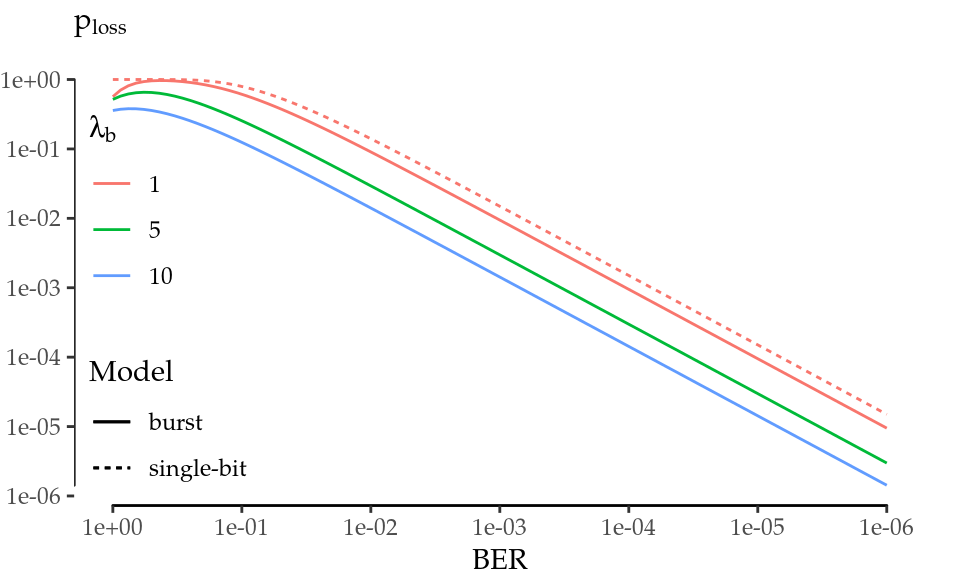
\includegraphics{05-unap_files/figure-latex/ploss-1} 

}

\caption[Frame loss probability given a BER level.]{Frame loss probability given a BER level.}\label{fig:ploss}
\end{marginfigure}

\section{\texorpdfstring{$\mu$}{\textmu}Nap Algorithm}\label{munap-algorithm}

In the following, we present \(\mu\)Nap, which builds upon the insights
provided in previous sections and tries to save energy during the
channel transmissions in which the STA is not involved. However, not all
transmissions addressed to other stations are eligible for dozing, as
the practical issues derived from the capture effect may incur in
performance degradation. Therefore, the algorithm must check both the
receiver as well as the transmitter address in the MAC header in order
to determine whether the incoming frame is addressed to another station
\emph{and} it comes from within the same network.

If these conditions are met, a basic micro-sleep will last the duration
of the rest of the incoming frame plus an inter-frame space (SIFS).
Unfortunately, the long times required to bring an interface back and
forth from sleep, as discovered in Section \ref{state-transition-times},
shows that this basic micro-sleep may not be long enough to be
exploitable. Thus, the algorithm should take advantage of the NAV field
whenever possible. Our previous analysis shows that this duration
information stored in the NAV is not exploitable in every circumstance:
the interface can leverage this additional time during CPs and it must
avoid any NAV set by a CTS packet.

Finally, after a micro-sleep, two possible situations arise:

\begin{itemize}
\tightlist
\item
  The card wakes up at the end of a frame exchange. For instance, after
  a data + ACK exchange. In this case, all STAs should wait for a DIFS
  interval before contending again.
\item
  The card wakes up in the middle of a frame exchange. For instance, see
  Figure \ref{fig:fragments}, where an RTS/CTS-based fragmented
  transmission is depicted.
\end{itemize}




\begin{figure}

{\centering 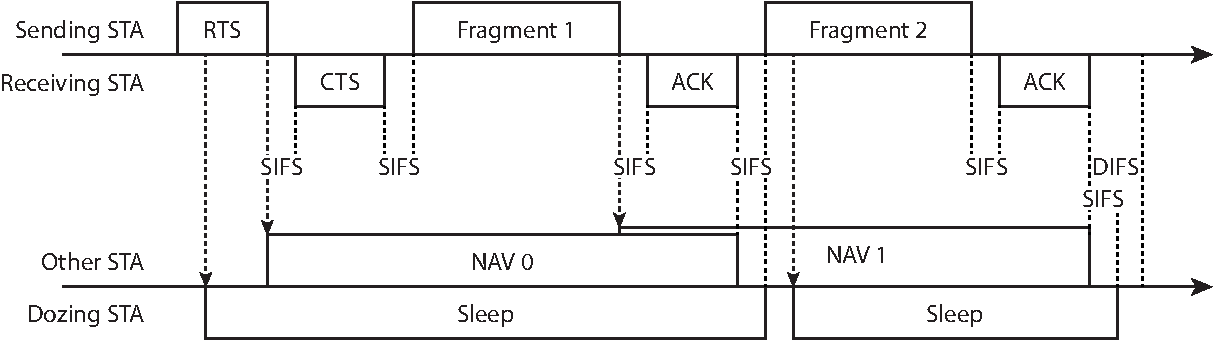
\includegraphics{img/05/fragments} 

}

\caption[RTS/CTS-based fragmented transmission example and
\(\mu\)Nap's behaviour.]{RTS/CTS-based fragmented transmission example and
\(\mu\)Nap's behaviour.}\label{fig:fragments}
\end{figure}

In the latter example, an RTS sets the NAV to the end of a fragment, and
our algorithm triggers the sleep. This first fragment sets the NAV to
the end of the second fragment, but it is not seen by the dozing STA.
When the latter wakes up, it sees a SIFS period of silence and then the
second fragment, which sets its NAV again and may trigger another sleep.
This implies that the STA can doze for an additional SIFS, as Figure
\ref{fig:fragments} shows, and wait in idle state until a DIFS is
completed before trying to contend again.

\newthought{Based on the above}, Algorithm \ref{fig:unap} describes the
main loop of a wireless card's microcontroller that would implement our
mechanism. When the first 16 bytes of the incoming frame are received,
all the information needed to take the decision is available: the
duration value (\(\Delta t_\mathrm{NAV}\)), the receiver address
(\(R_A\)) and the transmitter address (\(T_A\)). The ability to stop a
frame's reception at any point has been demonstrated to be
feasible\cite[0pt]{berger2014}\marginnote{\hypersetup{hidelinks}\color{white}\citet{berger2014}}.
Note that MAC addresses can be efficiently compared in a streamed way,
so that the first differing byte (if the first byte of the \(R_A\) has
the multicast bit set to zero, i.e., \(R_A\) is unicast) triggers our
sleep procedure (\texttt{Set\_Sleep} in Algorithm \ref{fig:unap}). In
addition, the main loop should keep up to date a global variable (\(C\))
indicating whether the contention is currently allowed (CP) or not
(CFP). This is straightforward, as every CFP starts and finishes with a
beacon frame.

The \texttt{Set\_Sleep} procedure takes as input the remaining time
until the end of the incoming frame (\(\Delta t_\mathrm{DATA}\)) and the
duration value (\(\Delta t_\mathrm{NAV}\)). The latter is used only if
it is a valid duration value and a CP is active. Then, the card may doze
during \(\Delta t_\mathrm{sleep}\) (if this period is greater than
\(\Delta t_\mathrm{sleep,min}\)), wait for a DIFS to complete and return
to the main loop.

Finally, it is worth noting that this algorithm is deterministic, as it
is based on a set of conditions to trigger the sleep procedure. It works
locally with the information already available in the protocol headers,
without incurring in any additional control overhead and without
impacting the normal operation of 802.11. Specifically, our analytical
study of the impact of errors in the first 16 bytes of the MAC header
shows that the probability of performance degradation is comparable to
the BER under normal channel conditions. Therefore, the overall
performance in terms of throughput and delay is completely equivalent to
normal 802.11.

\PSalgorithm{!h}{fig:unap}{$\mu$Nap implementation. Main loop modification to leverage micro-sleeps.}

\cleardoublepage

\hypertarget{performance-evaluation}{%
\section{Performance Evaluation}\label{performance-evaluation}}

This section is devoted to evaluate the performance of \(\mu\)Nap.
First, through trace-driven simulation, we show that \(\mu\)Nap
significantly reduces the overhearing time and the energy consumption in
a real network. Secondly, we analyse the impact of the timing
constraints imposed by the hardware, which are specially bad in the case
of the AR9280, and we discuss the applicability of \(\mu\)Nap in terms
of those parameters and the evolution trends in the 802.11 standard.

\hypertarget{evaluation-with-real-traces}{%
\subsection{Evaluation with Real
Traces}\label{evaluation-with-real-traces}}

In the following, we conduct an evaluation to assess how much energy
might be saved in a real network if all STAs implement \(\mu\)Nap using
the AR9280. The reasons for this are twofold. On the one hand, the
timing properties of this interface are particularly bad if we think of
typical frame durations in 802.11, which means that many micro-sleep
opportunities will be lost due to hardware constraints. On the other
hand, it does not support newer standards that could potentially lead to
longer micro-sleep opportunities through mechanisms such as frame
aggregation. Therefore, an evaluation based on an 11a/g network and the
AR9280 chip represents a worst case scenario for our algorithm.

For this purpose, we used 802.11a wireless traces with about 44 million
packets, divided in 43 files, from the SIGCOMM'08 data
set\cite[0pt]{umd-sigcomm2008-2009-03-02}\marginnote{\hypersetup{hidelinks}\color{white}\citet{umd-sigcomm2008-2009-03-02}}.
The methodology followed to parse each trace file is as follows.
Firstly, we discover all the STAs and APs present. Each STA is mapped
into its BSSID and a bit array is developed in order to hold the status
at each point in time (online or offline). It is hard to say when a
certain STA is offline from a capture, because they almost always
disappear without sending a disassociation frame. Thus, we use the
default rule in \texttt{hostapd}, the daemon that implements the AP
functionality in Linux: a STA is considered online if it transmitted a
frame within the last 5 min.

Secondly, we measure the amount of time that each STA spends (without
our algorithm) in the following states: transmission, reception,
overhearing and idle. We consider that online STAs are always awake;
i.e., even if a STA announces that it is going into PS mode, we ignore
this announcement. We measure also the amount of time that each STA
would spend (with our algorithm) in transmission, reception,
overhearing, sleep and idle. Transmission and reception times match the
previous case, as expected. As part of idle time, we account separately
the wasted time in each micro-sleep as a consequence of hardware
limitations (the fixed toll \(\Delta t_\mathrm{waste}\)). After this
processing, there are a lot of duplicate unique identifiers (MAC
addresses), i.e., STAs appearing in more than one trace file. Those
entries are summarised by aggregating the time within each state.

\newthought{At this point}, let us define the \emph{activity} time as
the sum of transmission, reception, overhearing, sleep and wasted time.
We do not take into account the idle time since our goal is to
understand how much power we can save in the periods of activity, which
are the only ones that consume power in wireless transmissions (the
scope of our mechanism). Using the definition above, we found that the
majority of STAs reveals very little activity (they are connected for a
few seconds and disappear). Therefore, we took the upper decile in terms
of activity, thus obtaining the 42 more active STAs.




\begin{figure*}

{\centering 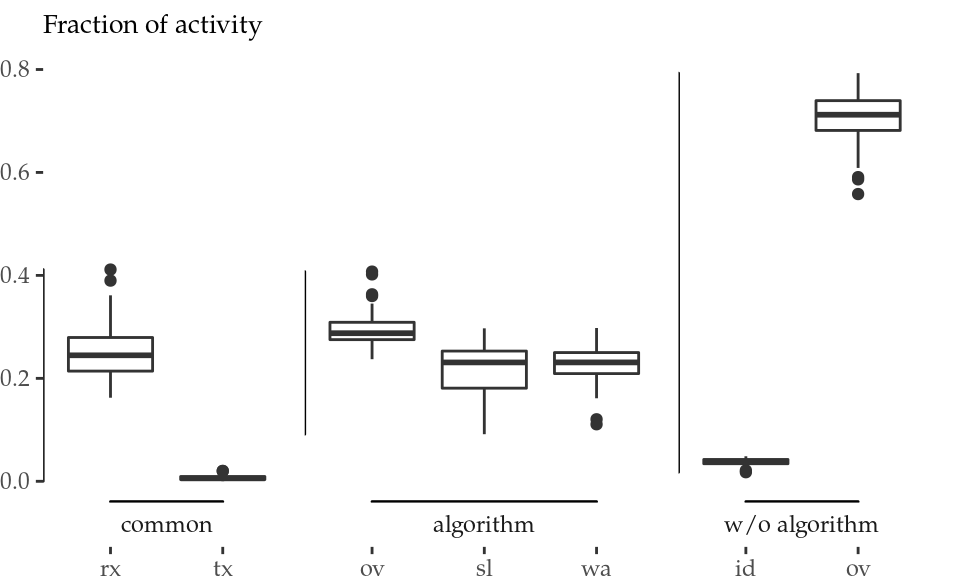
\includegraphics[width=0.49\linewidth]{05-unap_files/figure-latex/eval-agg-1} 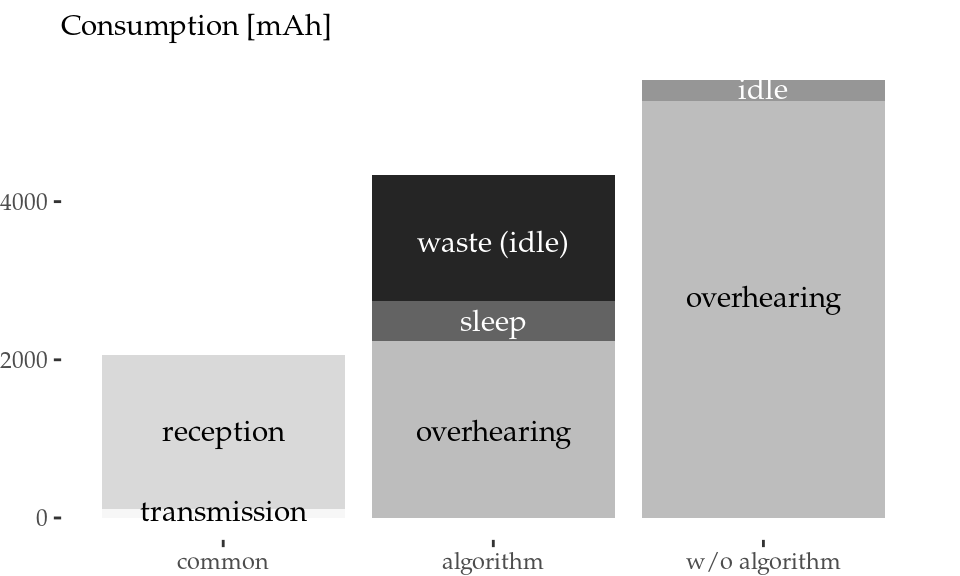
\includegraphics[width=0.49\linewidth]{05-unap_files/figure-latex/eval-agg-2} 

}

\caption[Normalised activity aggregation (left) and energy
consumption aggregation (right) of all STAs.]{Normalised activity aggregation (left) and energy
consumption aggregation (right) of all STAs.}\label{fig:eval-agg}
\end{figure*}

The activity aggregation of all STAs is normalised and represented in
Figure \ref{fig:eval-agg} (left). Transmission (tx) and reception (rx)
times are labelled as \emph{common}, because STAs spend the same time
transmitting and receiving both with and without our algorithm. It is
clear that our mechanism effectively reduces the total overhearing (ov)
time from a median of 70\% to a 30\% approximately (a 57\% reduction).
The card spends consistently less time in overhearing because this
overhearing time difference, along with some idle (id) time from
inter-frame spaces, turns into micro-sleeps, that is, sleep (sl) and
wasted (wa) time.

This activity aggregation enables us to calculate the total energy
consumption using the power values from the thorough characterisation
presented in Section \ref{characterisation-of-a-cots-device}. Figure
\ref{fig:eval-agg} (right) depicts the energy consumption in units of
mAh (assuming a typical 3.7-V battery). The energy savings overcome 1200
mAh even with the timing limitations of the AR9280 card, which (i)
prevents the card from going to sleep when the overhearing time is not
sufficiently long, and (ii) wastes a long fixed time in idle during each
successful micro-sleep. This reduction amounts to a 21.4\% of the energy
spent in overhearing and a 15.8\% of the total energy during the
activity time, when the transmission and reception contributions are
also considered.




\begin{figure*}

{\centering 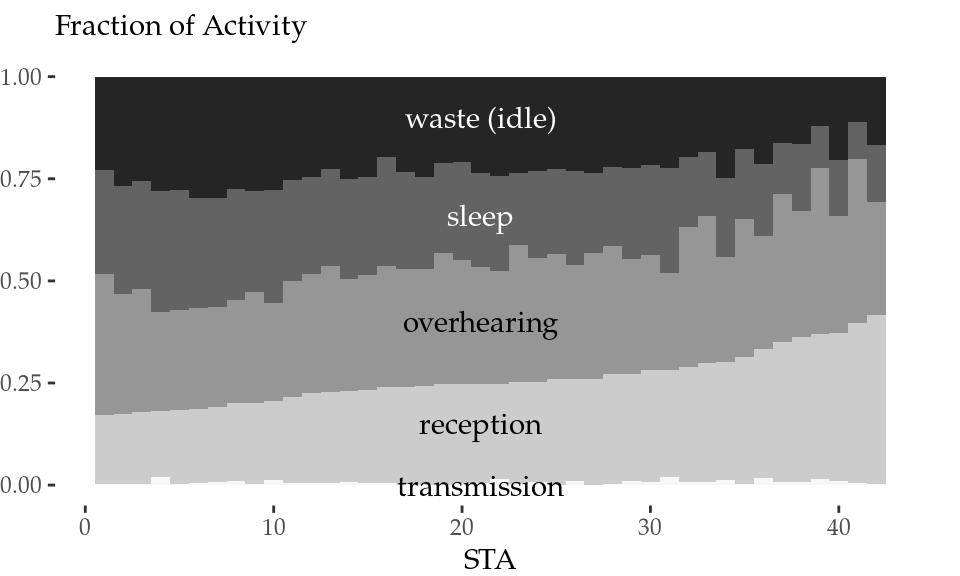
\includegraphics[width=0.49\linewidth]{05-unap_files/figure-latex/eval-sta-1} 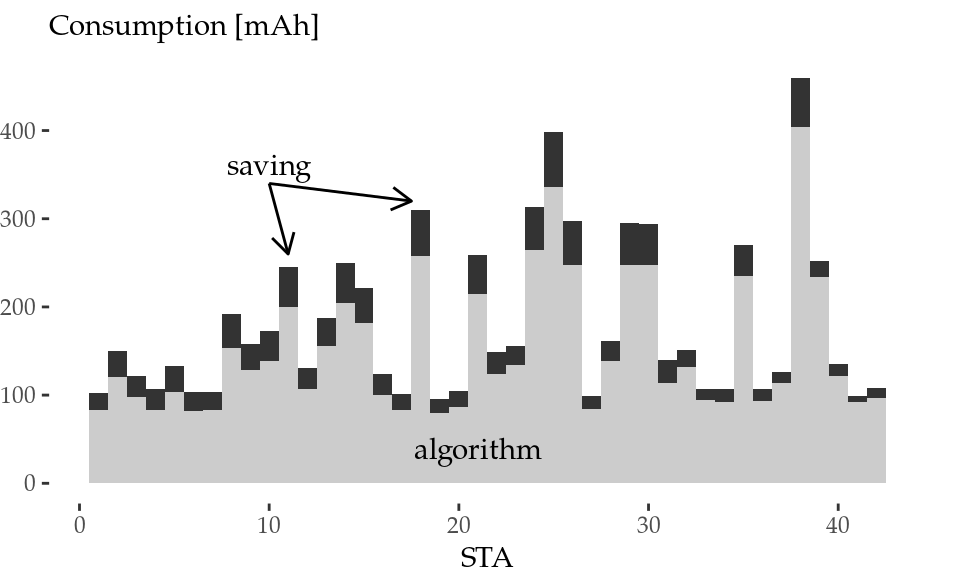
\includegraphics[width=0.49\linewidth]{05-unap_files/figure-latex/eval-sta-2} 

}

\caption[Normalised activity (left) and energy consumption (right)
per STA.]{Normalised activity (left) and energy consumption (right)
per STA.}\label{fig:eval-sta}
\end{figure*}

Figure \ref{fig:eval-sta} provides a breakdown of the data by STA. The
lower graph shows the activity breakdown per STA for our algorithm
(transmission bars, in white, are very small). Overhearing time is
reduced to a more or less constant fraction for all STAs (i.e., with the
algorithm, the overhearing bars represent more or less a 30\% of the
total activity for all STAs), while less participative STAs (left part
of the graph) spend more time sleeping. The upper graph shows the energy
consumption per STA with our algorithm along with the energy-saving in
dark gray, which is in the order of tens of mAh per STA.

\hypertarget{impact-of-timing-constraints}{%
\subsection{Impact of Timing
Constraints}\label{impact-of-timing-constraints}}

The performance gains of \(\mu\)Nap depend on the behaviour of the
circuitry. Its capabilities, in terms of timing, determine the maximum
savings that can be achieved. Particularly, each micro-sleep has an
efficiency (in comparison to an ideal scheme in which the card stays in
sleep state over the entire duration of the micro-sleep) given by
%
\begin{equation}
 \frac{E'_\mathrm{save}}{E_\mathrm{save}} = \frac{E_\mathrm{save} - E_\mathrm{waste}}{E_\mathrm{save}} \approx 1 - \frac{\Delta t_\mathrm{waste}}{\Delta t_\mathrm{sleep}}
 \label{eq:fracsave}
\end{equation}
%
which results from the combination of Equations \eqref{eq:idealsleep},
\eqref{eq:realsleep} and \eqref{eq:Ewaste}.

Figure \ref{fig:savings} represents this sleep efficiency for the AR9280
card (\(\Delta t_\mathrm{waste}=250\)) along with other values. It is
clear that an improvement of \(\Delta t_\mathrm{waste}\) is fundamental
to boost performance in short sleeps.




\begin{marginfigure}[-6in]

{\centering 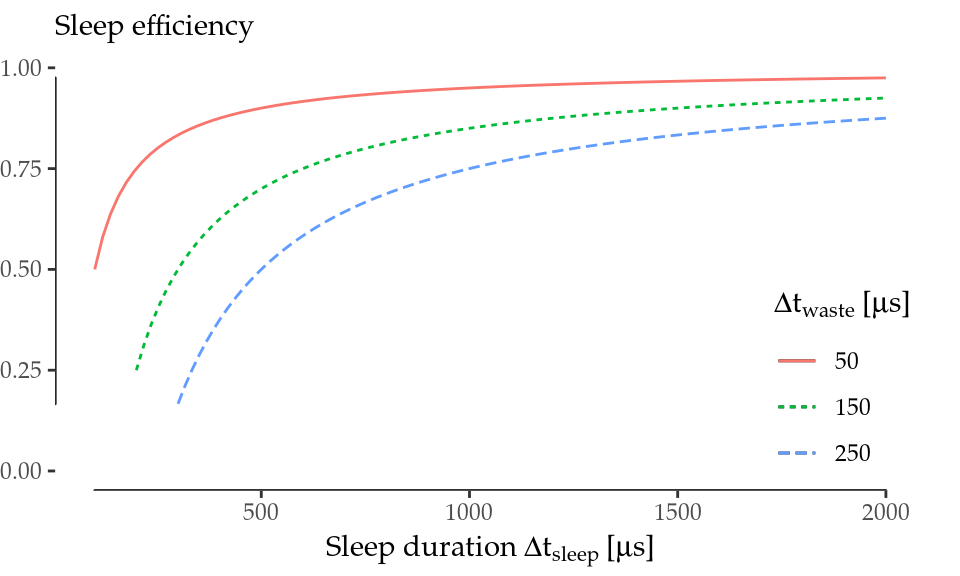
\includegraphics{05-unap_files/figure-latex/savings-1} 

}

\caption[Sleep efficiency \(E'_\mathrm{save}/E_\mathrm{save}\) as
\(\Delta t_\mathrm{waste}\) decreases.]{Sleep efficiency \(E'_\mathrm{save}/E_\mathrm{save}\) as
\(\Delta t_\mathrm{waste}\) decreases.}\label{fig:savings}
\end{marginfigure}

Similarly, the constraint \(\Delta t_\mathrm{sleep,min}\) limits the
applicability of \(\mu\)Nap, especially in those cases where the NAV
cannot be used to extend the micro-sleep. For instance, let us consider
the more common case in 11a/b/g networks: the transmission of a frame
(up to 1500 bytes long) plus the corresponding ACK. Then,
%
\begin{equation}
 \Delta t_\mathrm{sleep,min} \le \Delta t_\mathrm{DATA} + \Delta t_\mathrm{SIFS} + \Delta t_\mathrm{ACK} + \Delta t_\mathrm{SIFS} \label{eq:tsleepmin}
\end{equation}
%
and expanding the right side of the inequality,
%
\begin{equation*}
 \Delta t_\mathrm{sleep,min} \le \frac{8(14+l_\mathrm{min}+4)}{\lambda_\mathrm{DATA}} + \Delta t_\mathrm{PLCP} + \frac{8(14+2)}{\lambda_\mathrm{ACK}} + 2\Delta t_\mathrm{SIFS}
\end{equation*}
%


Here, we can find \(l_\mathrm{min}\), which is the minimum amount of
data (in bytes, and apart from the MAC header and the FCS) that a frame
must contain in order to last \(\Delta t_\mathrm{sleep,min}\). Based on
this \(l_\mathrm{min}\), Figure \ref{fig:applicability} defines the
applicability in 802.11a DCF in terms of frame sizes (\(\le 1500\)
bytes) that last \(\Delta t_\mathrm{sleep,min}\) at least. Again, an
improvement in \(\Delta t_\mathrm{waste}\) would boost not only the
energy saved per sleep, but also the general applicability defined in
this way.




\begin{figure*}

{\centering 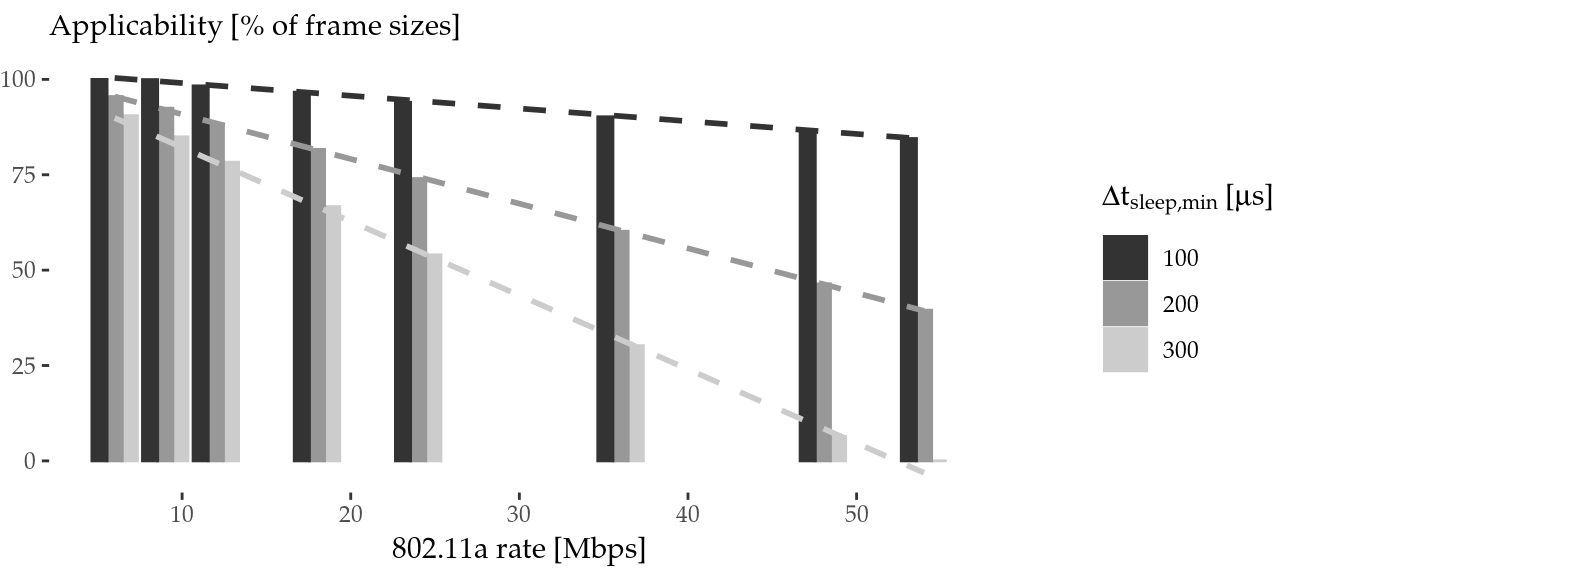
\includegraphics{05-unap_files/figure-latex/applicability-1} 

}

\caption[Algorithm applicability for common transmissions
(\(\le 1500\) bytes \(+\) ACK) in 802.11a DCF mode.]{Algorithm applicability for common transmissions
(\(\le 1500\) bytes \(+\) ACK) in 802.11a DCF mode.}\label{fig:applicability}
\end{figure*}

The applicability of \(\mu\)Nap may also be affected by the evolution of
the standard. Particularly, 802.11n introduced, and 802.11ac followed, a
series of changes enabling high and very high throughput respectively,
up to Gigabit in the latter case. This improvement is largely based on
MIMO and channel binding: multiple spatial and frequency streams.
Nevertheless, a single 20-MHz spatial stream is more or less equivalent
to 11ag. Some enhancements (shorter guard interval and coding
enhancements) may boost the throughput of a single stream from 54 to 72
Mbps under optimum conditions. Yet it is also the case that the PLCP is
much longer to accommodate the complexity of the new modulation coding
schemes (MCSs). This overhead not only extends each transmission, but
also encourages the use of frame aggregation. Thus, the increasing
bandwidth, in current amendments or future ones, does not necessarily
imply a shorter airtime in practice, and our algorithm is still valid.

\newthought{Reducing} PHY's timing requirements is essential to boost
energy savings, but its feasibility should be further investigated.
Nonetheless, there are some clues that suggest that there is plenty of
room for improvement. In the first place, \(\Delta t_\mathrm{off}\) and
\(\Delta t_\mathrm{on}\) should depend on the internal firmware
implementation (i.e., the complexity of saving/restoring the state).
Secondly, Figure \ref{fig:sleep-tx} (left) indicates that a transmission
is far more aggressive, in terms of a sudden power rise, than a return
from sleep. From this standpoint, \(\Delta t_\mathrm{ready} = 200\)
\(\mu\)s would be a pessimistic estimate of the time required by the
circuitry to stabilise. Last, but not least, the 802.3 standard goes
beyond 802.11 and, albeit to a limited extent, it defines some timing
parameters\footnote{E.g., \(\Delta t_\mathrm{w_{phy}}\) would be
  equivalent to our \(\Delta t_\mathrm{on}+\Delta t_\mathrm{ready}\).}
of the PHYs, which are in the range of tens of \(\mu\)s in the worst
case\footnote{See \citet[Table 78-4]{8023}}.

Due to these reasons, WiFi card manufacturers should push for a better
power consumption behaviour, which is necessary to boost performance
with the power-saving mechanism presented in this paper. Furthermore, it
is necessary for the standardisation committees and the manufacturers to
collaborate to agree on power consumption behaviour guidelines for the
hardware (similarly to what has been done with 802.3). Indeed, strict
timing parameters would allow researchers and developers to design more
advanced power-saving schemes.

\hypertarget{summary-2}{%
\section{Summary}\label{summary-2}}

Based on a thorough characterisation of the timing constraints and
energy consumption of 802.11 interfaces, we have exhaustively analysed
the micro-sleep opportunities that are available in current WLANs. We
have unveiled the practical challenges of these opportunities,
previously unnoticed in the literature, and, building on this knowledge,
we have proposed
\(\mu\)Nap\cite[0pt]{contrib-05a,contrib-05b}\marginnote{\hypersetup{hidelinks}\color{white}\citet{contrib-05a,contrib-05b}}
an energy-saving scheme that is orthogonal to the existing standard PS
mechanisms. Unlike previous attempts, our scheme takes into account the
non-zero time and energy required to move back and forth between the
active and sleep states, and decides when to put the interface to sleep
in order to make the most of these opportunities while avoiding frame
losses.

We have demonstrated the feasibility of our approach using a robust
methodology and high-precision instrumentation, showing that, despite
the limitations of COTS hardware, the use of our scheme would result in
a 57\% reduction in the time spent in overhearing, thus leading to an
energy saving of 15.8\% of the activity time according to our
trace-based simulation. Finally, based on these results, we have made
the case for the strict specification of energy-related parameters of
802.11 hardware, which would enable the design of platform-agnostic
energy-saving strategies.

\addtocontents{toc}{\partseparator}

\hypertarget{part-mathematical-modelling}{%
\part{Mathematical
Modelling}\label{part-mathematical-modelling}}

\hypertarget{ch:06}{%
\chapter{Rate Adaptation and Power Control in 802.11}\label{ch:06}}

\newthought{Rate adaptation} is a fundamental technique in 802.11
networks by which wireless transmistters adapt their transmission data
rate to the prevailing channel conditions. As we have learnt from
previous chapters, the energy consumption of wireless interfaces depends
on the chosen modulation and coding scheme, which defines the data rate.
On the other hand, \emph{transmission power control}, which has gained
increase attention due to network densification, tries to minimise the
amount of radiated power (and, indirectly, the energy consumption) given
a set of radio conditions.

These two competing techniques are typically assessed in terms of
throughput achieved, while it is assumed that optimality in terms of
this performance figure implies optimality in terms of energy
efficiency. This chapter tackles the latter question from a formal
standpoint. For this purpose, and we first present a joint goodput
(i.e., the throughtput delivered on top of 802.11) and energy
consumption model. Building on this model, we numerically study the
relationship between energy consumption and throughput performance in
802.11.

\hypertarget{joint-goodput-energy-model}{%
\section{Joint Goodput-Energy Model}\label{joint-goodput-energy-model}}

With the aim of isolating the variables of interest, namely, modulation
and coding scheme (MCS) and transmission power (TXP), in the following
we develop a joint goodput-energy model for a single 802.11 spatial
stream in the absence of interfering traffic. This model will let us
delve into the fundamental relationship between goodput and energy
consumption optimality without confounding effects such as collisions or
MIMO.

Beyond this primary intent, it is worth noting that these assumptions
conform with real-world scenarios in the scope of recent trends in the
IEEE 802.11 standard development (e.g., amendments 11ac and 11ad), where
device-to-device communications (mainly through beamforming and MU-MIMO)
are of paramount importance.

\pagebreak

We base our study on the work by \citet{Qiao2002}\cite{Qiao2002}, which
develops a robust goodput model that meets the established requirements.
This model analyses the IEEE 802.11a Distributed Coordination Function
(DCF) over the assumption of additive white Gaussian noise (AWGN)
channel without interfering traffic.

\newthought{Let us briefly introduce} the reader to the main concepts,
essential to our analysis, of the goodput model by \citet{Qiao2002}.
Given a packet of length \(l\) ready to be sent, a frame retry limit
\(n_\mathrm{max}\) and a set of channel conditions
\(\hat{s}=\{s_1, \ldots, s_{n_\mathrm{max}}\}\) and modulations
\(\hat{m}=\{m_1, \ldots, m_{n_\mathrm{max}}\}\) used during the
potential transmission attempts, the \emph{expected effective goodput}
\(\mathcal{G}\) is modelled as the ratio between the expected delivered
data payload and the expected transmission time as follows:
%
\begin{equation}
 \mathcal{G}(l, \hat{s}, \hat{m}) = \frac{{\mathbb E}\left[ \mathrm{data} \right]}{{\mathbb E}\left[ \mathcal{D}_\mathrm{data} \right]} = \frac{\Pr[\mathrm{succ} \mid l, \hat{s}, \hat{m}]\cdot l}{{\mathbb E}\left[ \mathcal{D}_\mathrm{data} \right]}
 \label{eq:goodput}
\end{equation}
%
where \(\Pr[\mathrm{succ} \mid l, \hat{s}, \hat{m}]\) is the probability
of successful transmission conditioned to \(l, \hat{s}, \hat{m}\), given
in \citet[Equation (5)]{Qiao2002}. This model is valid as long as the
coherence time is equal or greater than a single retry, i.e., the
channel condition \(s_i\) is constant.

The expected transmission time is defined as follows:
%
\begin{equation}
\begin{split}
 {\mathbb E}\left[ \mathcal{D}_\mathrm{data} \right] = \left(1 - \Pr[\mathrm{succ} \mid l, \hat{s}, \hat{m}]\right) \cdot \mathcal{D}_{\mathrm{fail} \mid l, \hat{s}, \hat{m}} \\
 + \Pr[\mathrm{succ} \mid l, \hat{s}, \hat{m}] \cdot \mathcal{D}_{\mathrm{succ} \mid l, \hat{s}, \hat{m}}
\end{split}
\label{eq:Ddata}
\end{equation}
%
where
%
\begin{equation}
\begin{split}
 \mathcal{D}_{\mathrm{succ} \mid l, \hat{s}, \hat{m}} = &\sum_{n=1}^{n_\mathrm{max}} \Pr[n \mathrm{~succ} \mid l, \hat{s}, \hat{m}] \cdot \biggl\lbrace \overline{T}_\mathrm{bkoff}(1) \biggr. \\
 &+ \sum_{i=2}^{n_\mathrm{max}} \left[\overline{T}_\mathrm{bkoff}(i)\right.+ \left.T_\mathrm{data}(l, m_i) + \overline{\mathcal{D}}_\mathrm{wait}(i)\right] \\
 &+ T_\mathrm{data}(l, m_1) + T_\mathrm{SIFS} + \biggl.T_\mathrm{ACK}(m'_n) + T_\mathrm{DIFS} \biggr\rbrace
\end{split}
\label{eq:Dsucc}
\end{equation}
%
is the average duration of a successful transmission and
%
\begin{equation}
 \mathcal{D}_{\mathrm{fail} \mid l, \hat{s}, \hat{m}} = \sum_{i=1}^{n_\mathrm{max}} \left[\overline{T}_\mathrm{bkoff}(i) + T_\mathrm{data}(l, m_i) + \overline{\mathcal{D}}_\mathrm{wait}(i+1)\right] 
\label{eq:Dfail}
\end{equation}
%
is the average time wasted during the \(n_\mathrm{max}\) attempts when
the transmission fails.

\(\Pr[n \mathrm{~succ} \mid l, \hat{s}, \hat{m}]\) is the probability of
successful transmission at the \(n\)-th attempt conditioned to
\(l, \hat{s}, \hat{m}\), and \(\overline{\mathcal{D}}_\mathrm{wait}(i)\)
is the average waiting time before the \(i\)-th attempt. Their
expressions are given in \citet[Equations (7)--(8)]{Qiao2002}. The
transmission time (\(T_\mathrm{data}\)), ACK time (\(T_\mathrm{ACK}\))
and average backoff time (\(\overline{T}_\mathrm{bkoff}\)) are given in
\citet[Equations (1)--(3)]{Qiao2002}. Finally, \(T_\mathrm{SIFS}\) and
\(T_\mathrm{DIFS}\) are 802.11a parameters, and they can be found also
in \citet[Table 2]{Qiao2002}.

\newthought{The selected energy model} is again the work by
\citet{Serrano2014}\cite{Serrano2014}, which stands as the most accurate
energy model for 802.11 devices published so far. While classical models
focused on the wireless interface solely, this one demonstrates
empirically that the energy consumed by the device itself cannot be
neglected as a device-dependent constant contribution. Conversely,
devices incur an energy cost derived from the frame processing, which
may impact the relationship that we want to evaluate in this paper.

\newthought{Putting together both models}, we are now in a position to
build a joint goodput-energy model for 802.11a DCF. Let us consider the
average durations \eqref{eq:Dsucc} and \eqref{eq:Dfail}. Based on their
expressions, we multiply the idle time
(\(\overline{\mathcal{D}}_\mathrm{wait}\),
\(\overline{T}_\mathrm{bkoff}\), \(T_\mathrm{SIFS}\),
\(T_\mathrm{DIFS}\)) by \(\rho_\mathrm{id}\), the transmission time
(\(T_\mathrm{data}\)) by \(\rho_\mathrm{tx}\), and the reception time
(\(T_\mathrm{ACK}\)) by \(\rho_\mathrm{rx}\). The resulting expressions
are the average energy consumed in a successful transmission
\(\mathcal{E}_{\mathrm{succ} \mid l, \hat{s}, \hat{m}}\) and the average
energy wasted when a transmission fails
\(\mathcal{E}_{\mathrm{fail} \mid l, \hat{s}, \hat{m}}\):
%
\begin{equation}
\begin{split}
 \mathcal{E}_{\mathrm{succ} \mid l, \hat{s}, \hat{m}} = &\sum_{n=1}^{n_\mathrm{max}} \Pr[n \mathrm{~succ} \mid l, \hat{s}, \hat{m}] \cdot \biggl\lbrace \rho_\mathrm{id}\overline{T}_\mathrm{bkoff}(1) \biggr. \\
 &+ \sum_{i=2}^{n_\mathrm{max}} \left[\rho_\mathrm{id}\overline{T}_\mathrm{bkoff}(i)\right.+ \left.\rho_\mathrm{tx}T_\mathrm{data}(l, m_i) + \rho_\mathrm{id}\overline{\mathcal{D}}_\mathrm{wait}(i)\right] \\
 &+ \rho_\mathrm{tx}T_\mathrm{data}(l, m_1) + \rho_\mathrm{id}T_\mathrm{SIFS} + \biggl.\rho_\mathrm{rx}T_\mathrm{ACK}(m'_n) + \rho_\mathrm{id}T_\mathrm{DIFS} \biggr\rbrace
\end{split}
\label{eq:Esucc}
\end{equation}
%
\begin{equation}
 \mathcal{E}_{\mathrm{fail} \mid l, \hat{s}, \hat{m}} = \sum_{i=1}^{n_\mathrm{max}} \left[\rho_\mathrm{id}\overline{T}_\mathrm{bkoff}(i) + \rho_\mathrm{tx}T_\mathrm{data}(l, m_i) + \rho_\mathrm{id}\overline{\mathcal{D}}_\mathrm{wait}(i+1)\right]
\label{eq:Efail}
\end{equation}
%


Then, by analogy with \eqref{eq:Ddata}, the \emph{expected energy consumed
per frame transmitted},
\({\mathbb E}\left[ \mathcal{E}_\mathrm{data} \right]\), can be written
as follows:
%
\begin{equation}
\begin{split}
 {\mathbb E}\left[ \mathcal{E}_\mathrm{data} \right] = \gamma_\mathrm{xg} + \left(1 - \Pr[\mathrm{succ} \mid l, \hat{s}, \hat{m}]\right) \cdot \mathcal{E}_{\mathrm{fail} \mid l, \hat{s}, \hat{m}} \\
 + \Pr[\mathrm{succ} \mid l, \hat{s}, \hat{m}] \cdot \mathcal{E}_{\mathrm{succ} \mid l, \hat{s}, \hat{m}}
\end{split}
\label{eq:energyperframe}
\end{equation}
%


It is noteworthy that the receiving cross-factor does not appear in this
expression because ACKs (acknowledgements) are processed in the network
card exclusively, and thus its processing toll is negligible.

Finally, we define the \emph{expected effective energy efficiency}
\(\mu\) as the ratio between the expected delivered data payload and the
expected energy consumed per frame, which can be expressed in \emph{bits
per Joule} (bpJ):
%
\begin{equation}
 \mu(l, \hat{s}, \hat{m}) = \frac{{\mathbb E}\left[ \mathrm{data} \right]}{{\mathbb E}\left[ \mathcal{E}_\mathrm{data} \right]}
 \label{eq:efficiency}
\end{equation}
%
\hypertarget{numerical-results}{%
\section{Numerical Results}\label{numerical-results}}

Building on the joint model presented in the previous section, here we
explore the relationship between optimal goodput and energy efficiency
in 802.11a. More specifically, our objective is to understand the
behaviour of the energy efficiency of a single spatial stream as the MCS
and TXP change following our model to meet the optimal goodput.

\hypertarget{optimal-goodput}{%
\subsection{Optimal Goodput}\label{optimal-goodput}}

We note that the main goal of RA, generally, is to maximise the
effective goodput that a station can achieve by varying the parameters
of the interface. In terms of the model discussed in the previous
section, a rate adaptation algorithm would aspire to fit the following
curve:
%
\begin{equation}
 \max{\mathcal{G}(l, \hat{s}, \hat{m})} \label{eq:maxgoodput}
\end{equation}
%


We provide the numerical results for this goodput maximisation problem
in Figure \ref{fig:maxgoodput}, which are in good agreement with those
obtained in \citet{Qiao2002}. For the sake of simplicity but without
loss of generality we fix \(l=1500\) octets and \(n_\mathrm{max}=7\)
retries, and assume that the channel conditions and the transmission
strategy are constant across retries (\(\hat{s}=\{s_1, \ldots, s_1\}\)
and \(\hat{m}=\{m_1, \ldots, m_1\}\)).

Figure \ref{fig:maxgoodput} illustrates which mode (see Table
\ref{tab:modes}) is optimal in terms of goodput, given an SNR level. We
next address the question of whether this optimisation is aligned with
energy efficiency maximisation.



\begin{figure}

{\centering 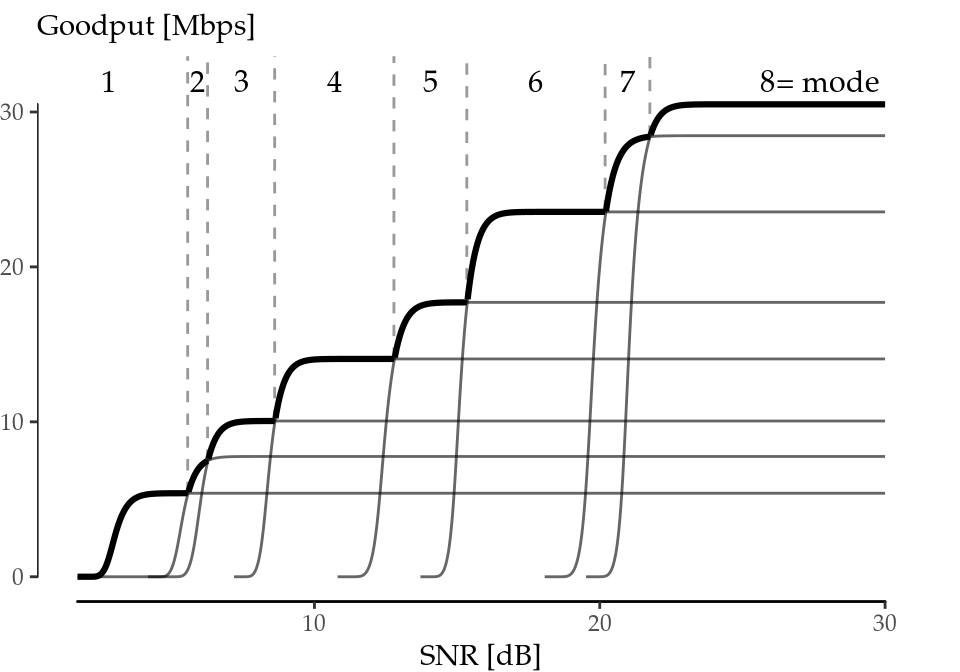
\includegraphics{06-ra-tpc_files/figure-latex/maxgoodput-1} 

}

\caption[Optimal goodput (bold envelope) as a function of SNR.]{Optimal goodput (bold envelope) as a function of SNR.}\label{fig:maxgoodput}
\end{figure}

\begin{margintable}[-2.68in]

\begin{center}
\resizebox{\linewidth}{!}{
\begin{tabular}{rrr}
\toprule
  & Mode Index & MCS [Mbps]\\
\midrule
 & 1 & 6\\
 & 2 & 9\\
 & 3 & 12\\
 & 4 & 18\\
 & 5 & 24\\
 & 6 & 36\\
 & 7 & 48\\
 & 8 & 54\\
\bottomrule
\end{tabular}}
\end{center}
\caption{\label{tab:modes}IEEE 802.11a PHY.}
\end{margintable}

\hypertarget{extension-of-the-energy-parametrisation}{%
\subsection{Extension of the Energy
Parametrisation}\label{extension-of-the-energy-parametrisation}}

The next step is to delve into the energy consumption of wireless
devices. \citet{Serrano2014} provides real measurements for five
devices: three AP-like platforms (Linksys WRT54G, Raspberry Pi and
Soekris net4826-48) and two hand-held devices (HTC Legend and Samsung
Galaxy Note 10.1). Two of the four parameters needed are constant
(\(\rho_\mathrm{id}, \gamma_\mathrm{xg}\)), and the other two
(\(\rho_\mathrm{tx}, \rho_\mathrm{rx}\)) depend on the MCS and the TXP
used. However, the characterisation done by \citet{Serrano2014} is
performed for a subset of the MCS and TXP available, so we next detail
how we extend the model to account for a larger set of operation
parameters.

A detailed analysis of the numerical figures presented in
\citet{Serrano2014} suggests that \(\rho_\mathrm{rx}\) depends linearly
on the MCS, and that \(\rho_\mathrm{tx}\) depends linearly on the MCS
and the TXP (in mW). Based on these observations, we define the
following linear models:
%
\begin{equation}
\begin{split}
 \rho_\mathrm{tx} &= \alpha_0 + \alpha_1\cdot\mathrm{MCS} + \alpha_2\cdot\mathrm{TXP} \\
 \rho_\mathrm{rx} &= \beta_0 + \beta_1\cdot\mathrm{MCS}
\end{split}
\label{eq:linearmodels}
\end{equation}
%


The models are fed with the data reported in \citet{Serrano2014}, and
the resulting fitting is illustrated in Figure \ref{fig:rho-tx-rx},
while Table \ref{tab:regressions-tx} collects the model estimates for
each device (with errors between parentheses), as well as the adjusted
r-squared. Since these linear models show a very good fit, they support
the generation of synthetic data for the different MCS and TXP required.





\begin{figure*}

{\centering 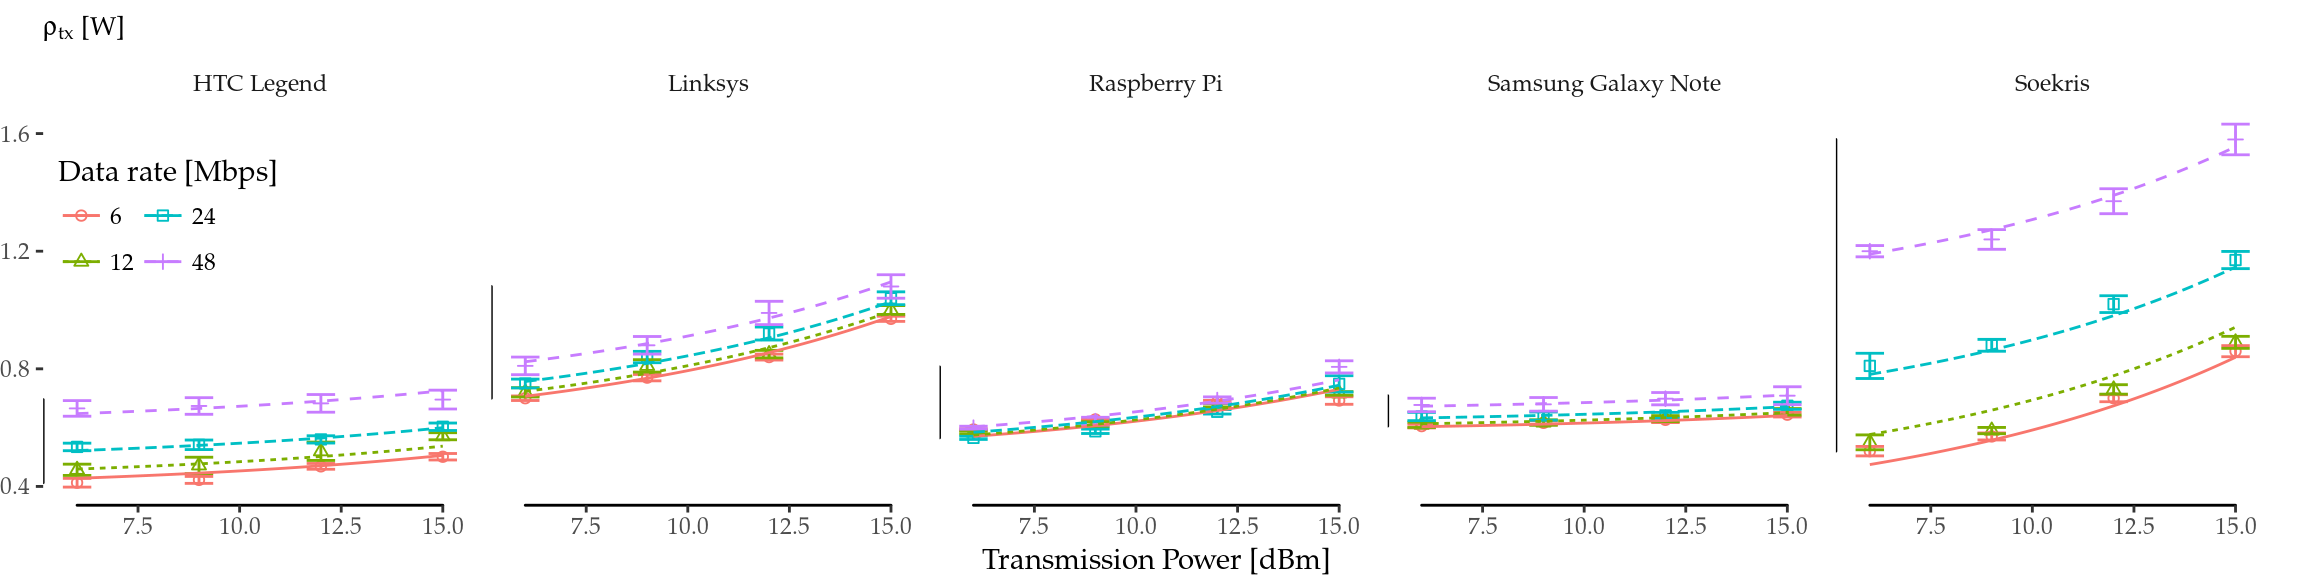
\includegraphics{06-ra-tpc_files/figure-latex/rho-tx-rx-1} 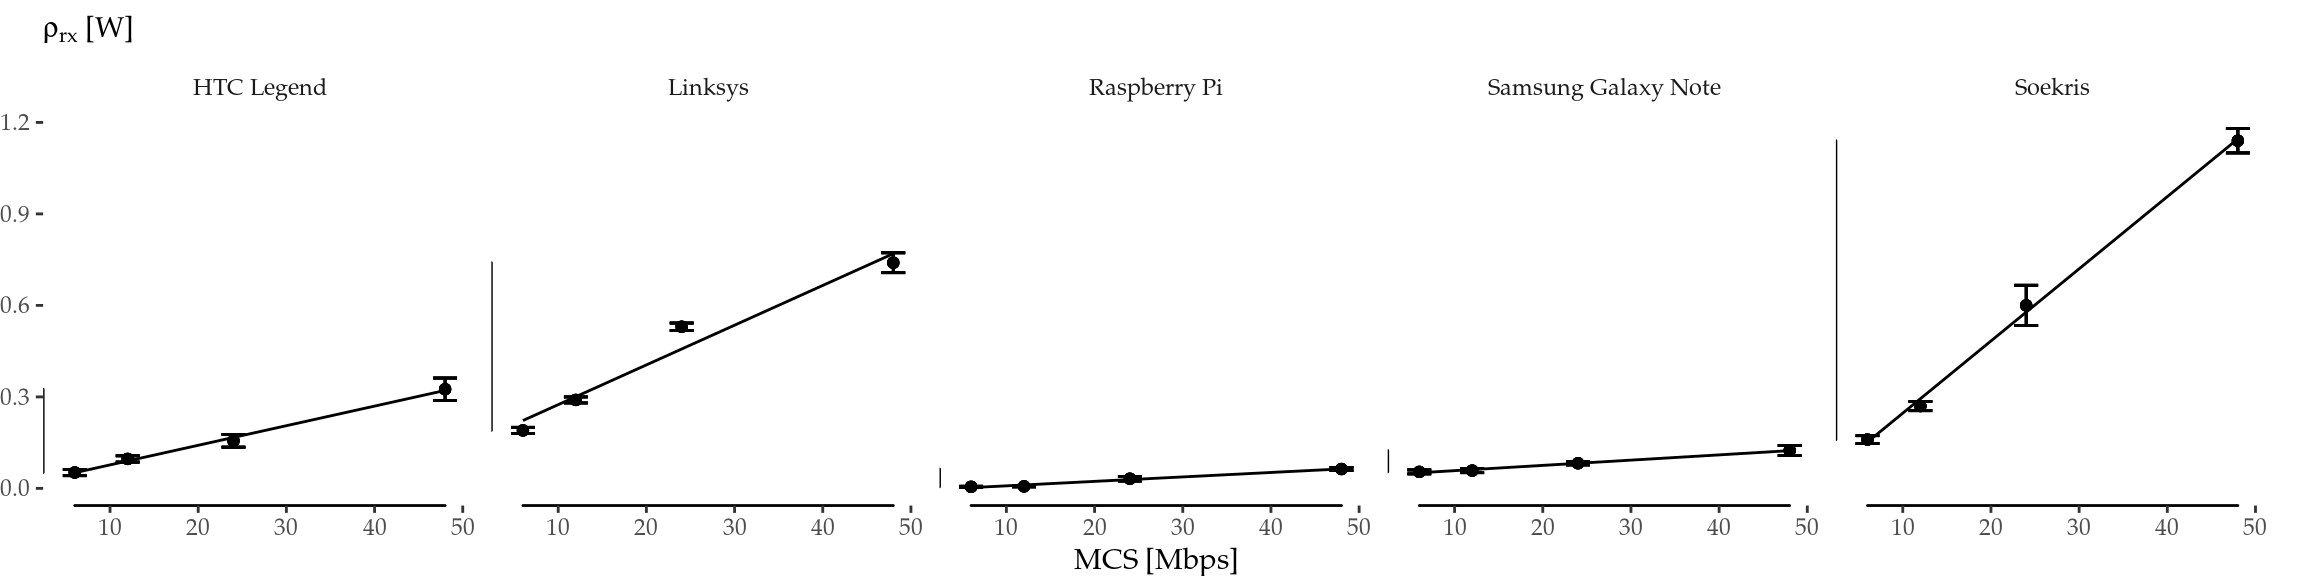
\includegraphics{06-ra-tpc_files/figure-latex/rho-tx-rx-2} 

}

\caption[Linear regressions. \(\rho_\mathrm{tx}\) fit as a
function of MCS and TXP (top) and \(\rho_\mathrm{rx}\) fit as a function
of MCS (bottom).]{Linear regressions. \(\rho_\mathrm{tx}\) fit as a
function of MCS and TXP (top) and \(\rho_\mathrm{rx}\) fit as a function
of MCS (bottom).}\label{fig:rho-tx-rx}
\end{figure*}

\begin{table*}

\begin{center}
\resizebox{\linewidth}{!}{
\begin{tabular}{rlllcllc}
\toprule
\multicolumn{1}{c}{ } & \multicolumn{4}{c}{$\rho_\mathrm{tx}$ model estimates} & \multicolumn{3}{c}{$\rho_\mathrm{rx}$ model estimates} \\
\cmidrule(l{2pt}r{2pt}){2-5} \cmidrule(l{2pt}r{2pt}){6-8}
Device & $\alpha_0$ [W] & $\alpha_1$ [W/Mbps] & $\alpha_2$ [W/mW] & adj. $r^2$ & $\beta_0$ [W] & $\beta_1$ [W/Mbps] & adj. $r^2$\\
\midrule
HTC Legend & 0.35(1) & 0.0052(3) & 0.021(3) & 0.966 & 0.013(3) & 0.0064(1) & 0.995\\
Linksys & 0.54(1) & 0.0028(2) & 0.075(3) & 0.982 & 0.14(2) & 0.0130(7) & 0.957\\
Raspberry Pi & 0.48(2) & 0.0008(4) & 0.044(5) & 0.866 & -0.006(1) & 0.00146(5) & 0.982\\
Samsung Galaxy Note & 0.572(4) & 0.00166(8) & 0.0105(9) & 0.975 & 0.041(1) & 0.00173(4) & 0.993\\
Soekris & 0.17(3) & 0.0170(6) & 0.101(7) & 0.986 & 0.010(8) & 0.0237(3) & 0.998\\
\bottomrule
\end{tabular}}
\end{center}
\vspace*{2mm}
\caption{\label{tab:regressions-tx}Linear regressions.}
\end{table*}

\hypertarget{energy-consumption}{%
\subsection{Energy Consumption}\label{energy-consumption}}

To compute the energy consumption using the above parametrisation, first
we have to define the assumptions for the considered scenario. We assume
for simplicity a device-to-device communication, with fixed and
reciprocal channel conditions during a sufficient period of time (i.e.,
low or no mobility). As we have discussed before, our primary goal is to
isolate MCS and TXP as variables of interest, but we must not forget
that these are also reasonable assumptions in scenarios targeted by
recent 802.11 standard developments (11ac, 11ad).

For instance, given channel state information from a receiver, the
transmitter may decide to increase the TXP in order to increase the
receiver's SNR (and thus the expected goodput), or to decrease it if the
channel quality is high enough. Although the actual relationship between
TXP and SNR depends on the specific channel model (e.g., distance,
obstacles, noise), without loss of generality, we choose a noise floor
of \(N=-85\) dBm in an office scenario with a link distance of \(d=18\)
m in order to explore numerically the whole range of SNR while using
reasonable values of TXP. The ITU model for indoor
attenuation\cite[-10mm]{iturp1238-2015}\marginnote{\hypersetup{hidelinks}\color{white}\citet{iturp1238-2015}}
gives a path loss of \(L\approx 85\) dBm. Then, we can use
\eqref{eq:energyperframe} to obtain the expected energy consumed per frame
and MCS mode, with TXP being directly related to the SNR level.




\begin{figure*}

{\centering 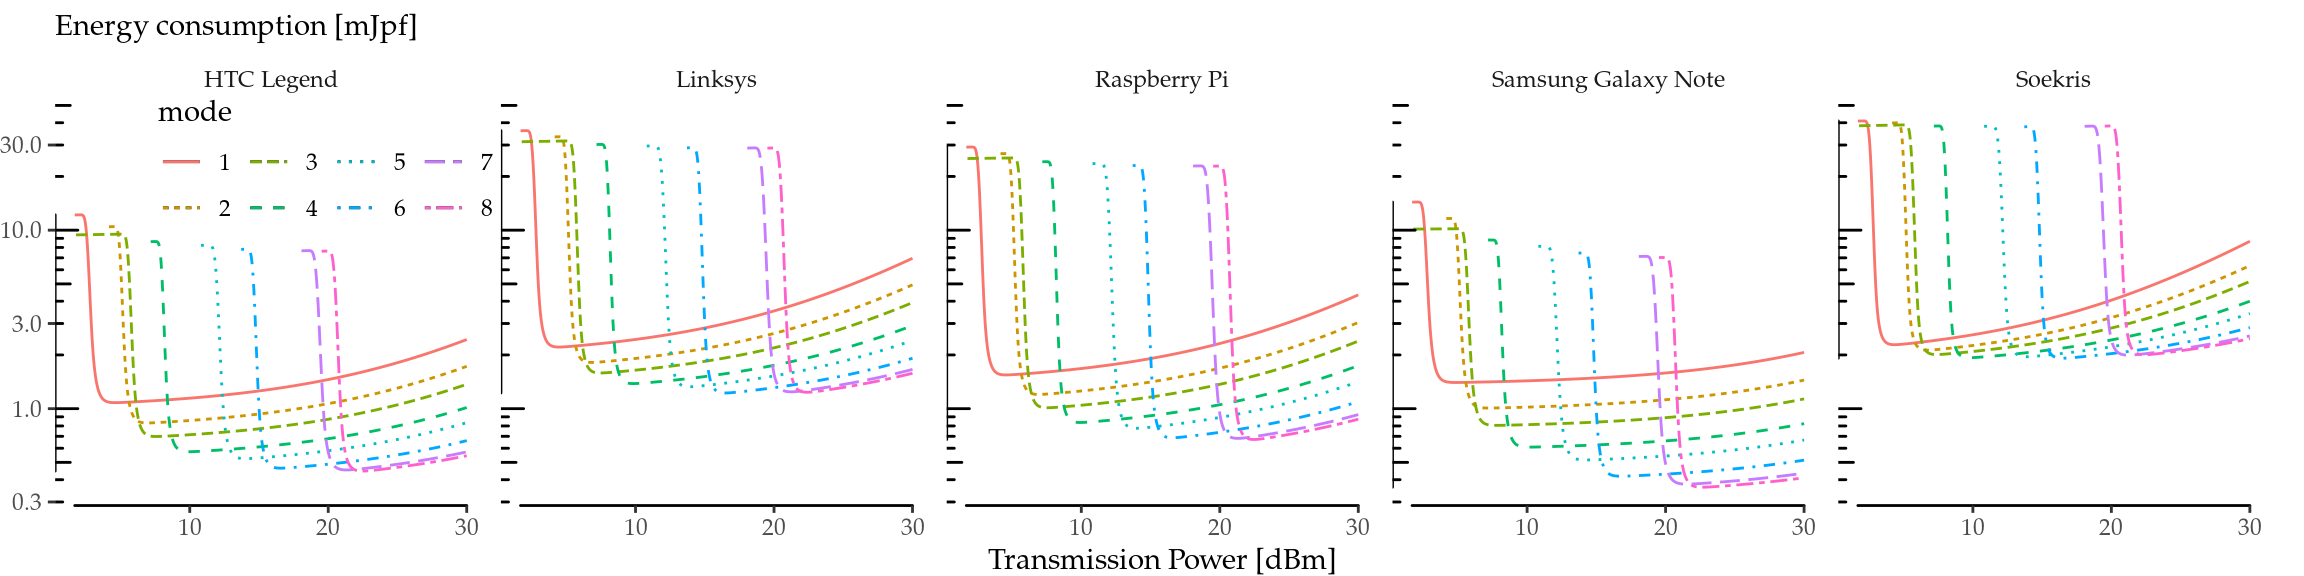
\includegraphics{06-ra-tpc_files/figure-latex/consumption-1} 

}

\caption[Expected energy consumption per frame in
\emph{millijoules per frame} (mJpf) under fixed channel conditions.]{Expected energy consumption per frame in
\emph{millijoules per frame} (mJpf) under fixed channel conditions.}\label{fig:consumption}
\end{figure*}

The results are reported in Figure \ref{fig:consumption}. As the figure
illustrates, consumption first falls abruptly as the TXP increases for
all modes, which is caused when the SNR reaches a sharp threshold level
such that the number of retransmissions changes from 6 to 0 (i.e., no
frame is discarded). From this threshold on, the consumption increases
with TXP because, although the number of retransmissions is 0, the
wireless interface consumes more power. We note that the actual value of
the TXP when the consumption drops depends on the specifics of the
scenario considered, but the qualitative conclusions hold for a variety
of scenarios.

\hypertarget{energy-efficiency-vs.optimal-goodput}{%
\subsection{Energy Efficiency vs.~Optimal
Goodput}\label{energy-efficiency-vs.optimal-goodput}}

We can finally merge previous numerical analyses and confront energy
efficiency, given by \eqref{eq:efficiency}, and optimal goodput, given by
\eqref{eq:maxgoodput}, for all devices and under the aforementioned
assumptions. To this aim, we plot in the same figure the energy
efficiency for the configuration that maximises goodput given an SNR
value vs.~the obtained goodput, with the results being depicted in
Figure \ref{fig:efficiency-goodput}. We next discuss the main findings
from the figure.




\begin{figure*}

{\centering 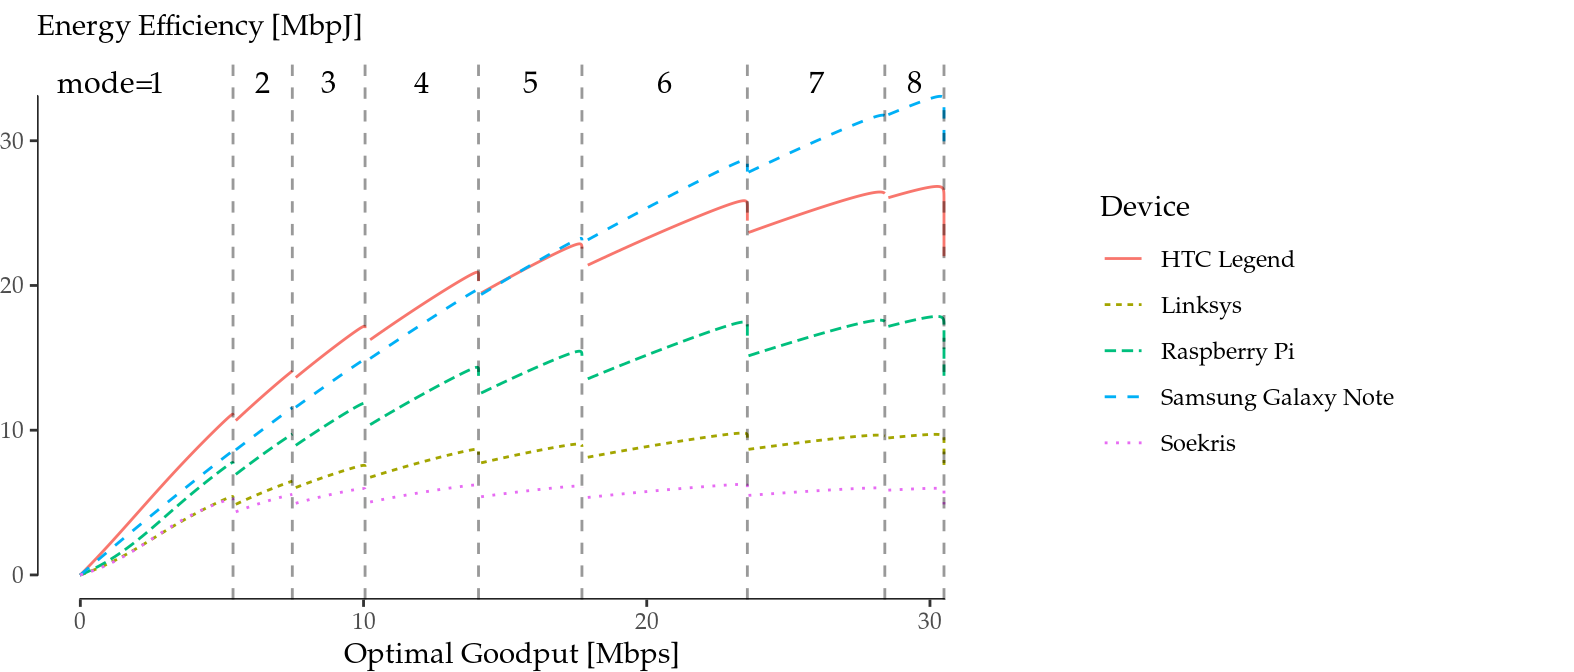
\includegraphics{06-ra-tpc_files/figure-latex/efficiency-goodput-1} 

}

\caption[Energy efficiency vs.~optimal goodput under
fixed channel conditions.]{Energy efficiency vs.~optimal goodput under
fixed channel conditions.}\label{fig:efficiency-goodput}
\end{figure*}

First of all, we can see that the energy efficiency grows sub-linearly
with the optimal goodput (the optimal goodput for each SNR value) in all
cases. We may distinguish three different cases in terms of energy
efficiency: high (Samsung Galaxy Note and HTC Legend), medium (Raspberry
Pi) and low energy efficiency (Linksys and Soekris). Furthermore, for
the case of the Soekris, we note that the ``central modes'' (namely, 4
and 5) are more efficient in their optimal region than the subsequent
ones.

Another finding (more relevant perhaps) is that it becomes evident that
increasing the goodput does not always improve the energy efficiency:
there are more or less drastic leaps, depending on the device, between
mode transitions. From the transmitter point of view, in the described
scenario, this can be read as follows: we may increase the TXP to
increase the SNR, but if the optimal goodput entails a mode transition,
the energy efficiency may be affected.

As a conclusion, we have demonstrated that optimal goodput and energy
efficiency do not go hand in hand, even in a single spatial stream, in
802.11\footnote{These findings have been further confirmed with an
  experimental validation, which is covered in Appendix
  \ref{experimental-validation-of-ra-tpc-inefficiencies}.}. There is a
trade-off in some circumstances that current rate adaptation algorithms
cannot take into account, as they are oblivious to the energy
consumption characteristic of the device.

\hypertarget{discussion}{%
\section{Discussion}\label{discussion}}

\hypertarget{sensitivity-to-energy-parameter-scaling}{%
\subsection{Sensitivity to Energy Parameter
Scaling}\label{sensitivity-to-energy-parameter-scaling}}

We next explore how the different energy parameters affect the energy
efficiency vs.~optimal goodput relationship. For this purpose, we
selected the Raspberry Pi curve from Figure \ref{fig:efficiency-goodput}
(results are analogous with the other devices) and we scale up and down,
one at a time, the four energy parameters \(\rho_\mathrm{id}\),
\(\rho_\mathrm{tx}\), \(\rho_\mathrm{rx}\), and \(\gamma_\mathrm{xg}\).
The scaling up and down is done by multiplying and dividing by 3,
respectively, the numerical value of the considered parameter. One of
the first results is that the impact of \(\rho_\mathrm{rx}\) is
negligible, a result somehow expected as the cost of receiving the ACK
is practically zero. From this point on, we do not further consider this
parameter.




\begin{figure*}

{\centering 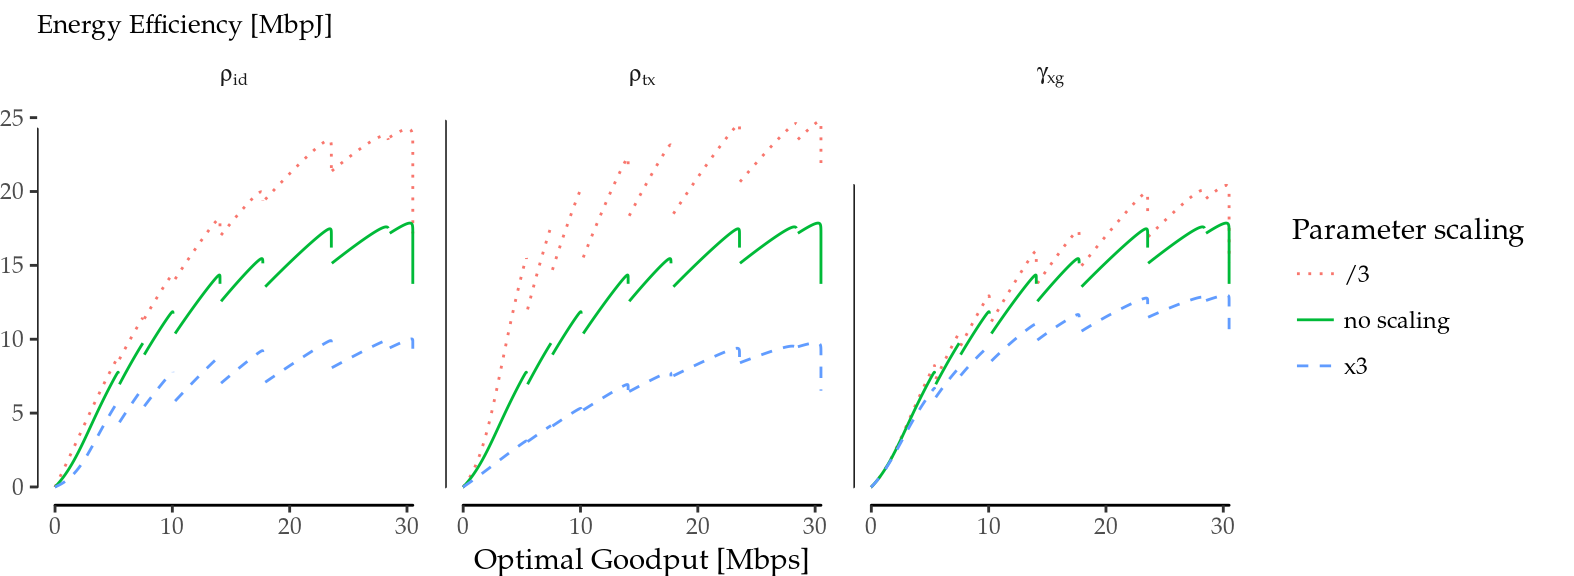
\includegraphics{06-ra-tpc_files/figure-latex/param-scaling1-1} 

}

\caption[Impact of energy parameter scaling on the energy
efficiency. Overall effect.]{Impact of energy parameter scaling on the energy
efficiency. Overall effect.}\label{fig:param-scaling1}
\end{figure*}

We show in Figure \ref{fig:param-scaling1} the overall effect of this
parameter scaling. The solid line represents the base case with no
scaling (same curve as in Figure \ref{fig:efficiency-goodput}), and in
dashed and dotted lines the corresponding parameter was multiplied or
divided by a factor of 3, respectively. As expected, larger parameters
contribute to lower the overall energy efficiency. However, the impact
on the energy efficiency drops between mode transitions is far from
being obvious, as in some cases transitions are more subtle while in
others they become more abrupt.




\begin{figure*}

{\centering 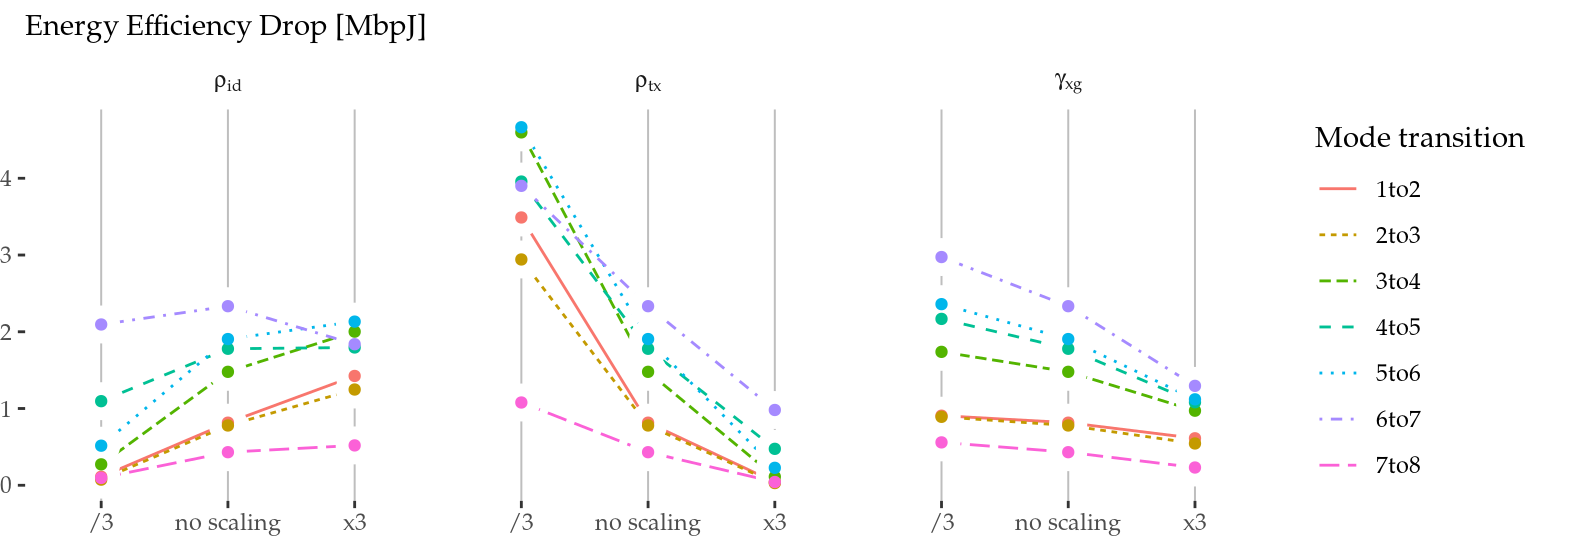
\includegraphics{06-ra-tpc_files/figure-latex/param-scaling2-1} 

}

\caption[Impact of energy parameter scaling on the energy
efficiency. Impact on mode transitions.]{Impact of energy parameter scaling on the energy
efficiency. Impact on mode transitions.}\label{fig:param-scaling2}
\end{figure*}

To delve into these transitions, we illustrate in Figure
\ref{fig:param-scaling2} the ``drop'' in energy efficiency when changing
between modes. As it can be seen, the cross-factor
\(\gamma_\mathrm{xg}\) is the less sensitive parameter of the three,
because its overall effect is limited and, more importantly, it scales
all the leaps between mode transitions homogeneously. This means that a
higher or lower cross-factor, which resides almost entirely in the
device and not in the wireless card, does not alter the energy
efficiency vs.~optimal goodput relationship\footnote{Note that this
  parameter results in a constant term in Equation
  \eqref{eq:energyperframe}.}. Thus, the cross-factor is not relevant from
the RA-TPC point of view, and energy-aware RA-TPC algorithms can be
implemented by leveraging energy parameters local to the wireless card.

On the other hand, \(\rho_\mathrm{id}\) and \(\rho_\mathrm{tx}\) have a
larger overall effect, plus an inhomogeneous and, in general, opposite
impact on mode transitions. While a larger \(\rho_\mathrm{id}\)
contributes to larger leaps, for the case of \(\rho_\mathrm{tx}\), the
larger energy efficiency drops occur with smaller values of that
parameter. Still, the reason behind this behaviour is the same for both
cases: the wireless card spends more time in idle (and less time
transmitting) when a transition to the next mode occurs, which has a
higher data rate.

This effect is also evident if we compare the Samsung Galaxy Note and
the HTC Legend curves in Figure \ref{fig:efficiency-goodput}. Both
devices have \(\rho_\mathrm{id}\) and \(\rho_\mathrm{tx}\) in the same
order of magnitude, but the HTC Legend has a larger \(\rho_\mathrm{id}\)
and a smaller \(\rho_\mathrm{tx}\). The combined outcome is a more
dramatic sub-linear behaviour and an increased energy efficiency drop
between mode transitions.

\hypertarget{heuristics-for-ra-tpc-algorithms}{%
\subsection{Heuristics for RA-TPC
Algorithms}\label{heuristics-for-ra-tpc-algorithms}}

We have seen that the energy efficiency vs.~optimal goodput relationship
shows a signature ``sawtooth'' pattern when RA and TPC are considered
for a single 802.11 spatial stream. This sawtooth shape presents a
growing trend in the central part of each mode, but there are energy
efficiency drops between mode transitions, which conceal a trade-off.

Parameter scaling has diverse effects on the final consumption
signature, but overall, the qualitative behaviour (i.e., the shape)
remains the same. The cross-factor produces an homogeneous scaling of
the sawtooth. Thus, a first conclusion is that the trade-off depends on
the energy parameters local to the wireless card, which means that a
properly designed energy-aware RA-TPC algorithm can be device-agnostic.

Moreover, an energy-aware RA-TCP algorithm may also be card-agnostic.
This is because the inefficiencies are always constrained at mode
transitions, which are exactly the points at which RA-TPC algorithms
take decisions. Therefore, there is no need of knowing the exact energy
parametrisation, nor the instantaneous power consumption of the wireless
card, in order to take energy-efficient decisions.

An RA-TPC algorithm moves along the sawtooth shapes of Figure
\ref{fig:efficiency-goodput} in two directions, namely, ``up'' (towards
higher throughput) and ``down'' (towards lower throughput). In this way,
an algorithm requires different policies to make a decision:

\begin{enumerate}
\def\labelenumi{(\roman{enumi})}
\tightlist
\item
  In the \emph{upwards} direction, in which mode transitions take place
  by increasing MCS and TXP (to achieve more goodput), a sensitive
  policy would be to remain in the left side of the leaps, to prevent
  falling into the efficiency gaps, until the link is good enough to
  move to a higher MCS with at least the same efficiency. An heuristic
  for the \emph{upwards} policy may be the following: whenever an
  algorithm chooses a higher MCS, it may hold the decision for some time
  and, if it persists, then trigger the MCS change\footnote{However, if
    this delay is too long, the algorithm will incur in inefficiencies,
    too.}.
\item
  In the \emph{downwards} direction, in which mode transitions take
  place by decreasing MCS and TXP, a sensitive policy would be to try to
  reach the left side of the leaps as soon as possible. However, it
  should be noted that this \emph{downwards} policy is much more
  challenging, as it implies predicting quality drops to trigger early
  MCS/TXP changes.
\end{enumerate}

In summary, our results suggest that one of the key points of an
energy-aware RA-TPC algorithm is the management of mode transitions. A
good algorithm should be \emph{conservative} at mode transitions, in the
sense that it should prefer a lower MCS and TXP until a higher MCS can
be guaranteed.

\hypertarget{summary-3}{%
\section{Summary}\label{summary-3}}

We have revisited 802.11 rate adaptation and transmission power control
by taking energy consumption into account. While some previous studies
pointed out that MIMO rate adaptation is not energy efficient, we have
demonstrated through numerical analysis that, even for single spatial
streams without interfering traffic, energy consumption and throughput
performance are different optimisation objectives.

Our
findings\cite[0pt]{contrib-06}\marginnote{\hypersetup{hidelinks}\color{white}\citet{contrib-06}}
show that this trade-off emerges at certain ``mode transitions'' when
maximising the goodput, suggesting that small goodput degradations may
lead to energy efficiency gains. For instance, a station at the edge of
a mode transition may decide to reduce the transmission power a little
in order to downgrade the modulation coding scheme. Or an opportunity to
achieve a better goodput by increasing the transmission power and
modulation coding scheme could be delayed if the expected gain is small.

\addtocontents{toc}{\partseparator}

\hypertarget{part-simulation}{%
\part{Simulation}\label{part-simulation}}

\hypertarget{ch:07}{%
\chapter{Performance of RA-TPC Algorithms in 802.11}\label{ch:07}}

\newthought{So far}, we have demonstrated through numerical analysis,
and validated experimentally\footnote{See Appendix
  \ref{experimental-validation-of-ra-tpc-inefficiencies}.}, the
existence of a trade-off between two competing performance figures,
namely, goodput and energy efficiency. This issue arises even for a
single spatial stream in absence of interference. Furthermore, we have
discussed in Section \ref{heuristics-for-ra-tpc-algorithms} some ideas
about the kind of mechanisms that energy-aware RA-TPC algorithms may
incorporate, to leverage the behaviour that we have identified in our
analysis in these so-called \emph{mode transitions}. Summing up, the
algorithms should be \emph{conservative} during these transitions.

During that discussion, we neglected the challenge of estimating channel
conditions. But in practice, any RA-TPC algorithm has imperfect channel
knowledge, and therefore will adapt to changing conditions in a
suboptimal way. In this chapter, we will analyse and compare the
performance of several representative existing RA algorithms, which also
incorporate TPC, to confirm whether the \emph{conservativeness} in such
decisions may have a positive impact on the achieved performance.

In the following, we first present the algorithms considered and
describe a simple simulation scenario to test them. Our results will
lead us to a more detailed discussion about \emph{conservativeness} at
mode transitions.

\hypertarget{algorithms-considered}{%
\section{Algorithms Considered}\label{algorithms-considered}}

If we take a look at the actual operation of WiFi networks, the
Minstrel\cite[0pt]{minstrel}\marginnote{\hypersetup{hidelinks}\color{white}\citet{minstrel}}
algorithm, which was integrated into the Linux kernel, has become the
\emph{de facto} standard due to its relatively good performance and
robustness. However, Minstrel does not consider TPC and, in consequence,
there is no TPC in today's WiFi deployments. Moreover, despite some
promising proposals have been presented in the literature, there are
very few of them implemented, although there are some ongoing efforts
such as the work by the authors of \emph{Minstrel-Piano}
\citep{huehn2012}, who are pushing to release an enhanced version of the
latter for the Linux kernel with the goal of promoting it
upstream.\footnote{\url{https://github.com/thuehn/Minstrel-Blues}}

As already stated, RA is a very prolific research line in the
literature, but the main corpus is dedicated to the MCS adjustment
without taking into account the TXP\footnote{See \citet{biaz2008} for a
  survey.}. There is some work considering TPC, but the motivation is
typically the performance degradation due to network densification, and
the aim is interference mitigation and not energy efficiency. Given that
we are interested in assessing RA implementations with TPC support, we
consider only open-source algorithms that can be tested using the NS-3
Network Simulator\footnote{\url{https://www.nsnam.org}}. After a
thorough analysis of the literature, we considered the following set of
algorithms:

\begin{description}
\tightlist
\item[Power-controlled Auto Rate Fallback]
(PARF),\cite[0pt]{Akella:2005}\marginnote{\hypersetup{hidelinks}\color{white}\citet{Akella:2005}}
which is based on \emph{Auto Rate Fallback} (ARF)
\citep{kamerman1997wavelan}, one of the earliest RA schemes for 802.11.
ARF rate adaptation is based on the frame loss ratio. It tunes the MCS
in a very straightforward and intuitive way. The procedure starts with
the lowest possible MCS. Then, if either a timer expires or the number
of consecutive successful transmissions reach a threshold, the MCS is
increased and the timer is reset. The MCS is decreased if either the
first transmission at a new rate fails or two consecutive transmissions
fail. PARF builds on ARF and tries to reduce the TXP if there is no loss
until a minimum threshold is reached or until transmissions start to
fail. If transmission fails persist, the TXP is increased.
\item[Minstrel-Piano]
(MP)\cite[0pt]{huehn2012}\marginnote{\hypersetup{hidelinks}\color{white}\citet{huehn2012}}
is based on Minstrel \citep{minstrel}. Minstrel performs per-frame rate
adaptation based on throughput. It randomly probes the MCS space and
computes an exponential weighted moving average (EWMA) on the
transmission probability for each rate, in order to keep a long-term
history of the channel state. As the previous algorithm, MP adds TPC
without interfering with the normal operation of Minstrel. It
incorporates to the TPC the same concepts and techniques than Minstrel
uses for the MCS adjustment, i.e., it tries to learn the impact of the
TXP on the achieved throughput.
\item[Robust Rate and Power Adaptation Algorithm]
(RRPAA) and \emph{Power, Rate and Carrier-Sense Control}
(PRCS),\cite[0pt]{richart2015}\marginnote{\hypersetup{hidelinks}\color{white}\citet{richart2015}}
which are based on \emph{Robust Rate Adaptation Algorithm} (RRAA)
\citep{Wong2006}. RRAA consists of two functional blocks, namely, rate
adaptation and collisions elimination. It performs rate adaptation based
on loss ratio estimation over short windows, and reduces collisions with
a RTS-based strategy. The procedure starts at the maximum MCS. The loss
ratio for each window of transmissions is available for rate adjustment
in the next window. There are two thresholds involved in this
adjustment: if the loss ratio is below both of them, the MCS is
increased; if it is above, the MCS is decreased; and if it is in
between, the MCS remains unchanged. RRPAA and PRCS build on this and try
to use the lowest possible TXP without degrading the throughput. For
this purpose, they firstly find the best MCS at the maximum TXP and,
from there, they jointly adjust the MCS and TXP for each window based on
a similar thresholding system. RRPAA and PRCS are very similar and only
differ in implementation details.
\end{description}

Based on their behaviour, these algorithms can be classified into three
distinct classes. First of all, MP is the most aggressive technique,
given that it constantly samples the whole MCS/TXP space searching for
the best possible configuration. On the opposite end, RRPAA and PRCS do
not sample the whole MCS/TXP space. Instead, they are based on a
windowed estimation of the loss ratio, which makes the MCS/TXP
transitions much lazier. Finally, PARF falls in between, as it changes
the MCS/TXP to the next available proactively if a number of
transmissions are successful, but it falls back to the previous one if
the new one fails. In practice, this may result in some instability
during transitions.

\hypertarget{simulation-scenario}{%
\section{Simulation Scenario}\label{simulation-scenario}}

This evaluation is publicly available,\footnote{\url{https://github.com/Enchufa2/ns-3-dev-git}}
and builds upon the code provided by \citet{richart2015}\footnote{\url{https://github.com/mrichart/ns-3-dev-git}}.
We assessed the proposed algorithms in the toy scenario depicted in
Figure \ref{fig:simulation}. It consists of a single access point (AP)
and a single mobile node connected to this AP configured with the
802.11a PHY. The mobile node at the farthest distance at which is able
to communicate at the lowest possible rate (6 Mbps) and highest TXP (17
dBm), and then it moves at constant speed towards the AP. The simulation
stops when the node is directly in front of the AP and it is able to
communicate at the highest possible rate (54 Mbps) and lowest TXP (0
dBm). This way, we sweep through all mode transitions available.



\begin{marginfigure}

{\centering 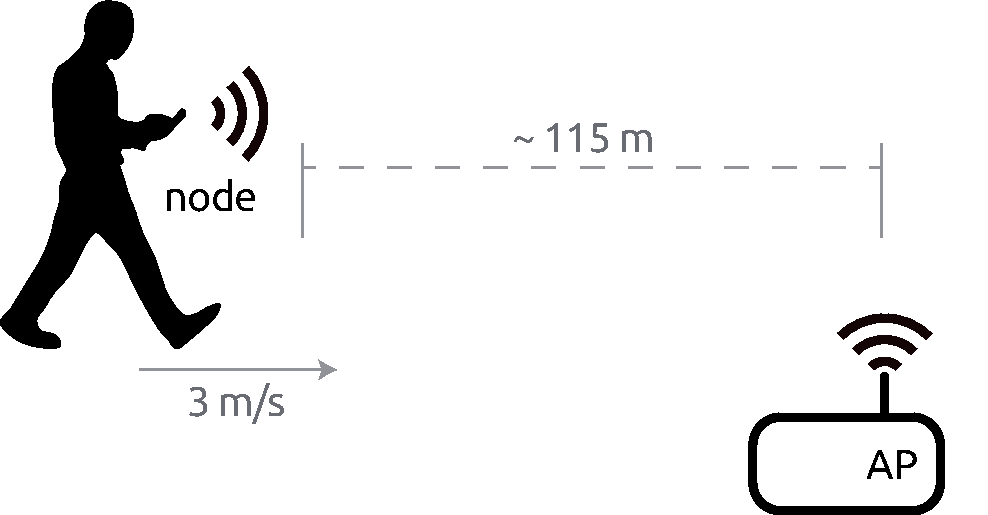
\includegraphics[width=1\linewidth]{img/07/simulation} 

}

\caption[Simulation scenario.]{Simulation scenario.}\label{fig:simulation}
\end{marginfigure}

For the whole simulation, the AP tries to constantly saturate the
channel by sending full-size UDP packets to the node. Every transmission
attempt is monitored, as well as every successful transmission. The
first part allows us to compute the transmission time, while the latter
allows us to compute the reception time (of the ACKs) and the goodput
achieved.

The simulation model assembles the power model from Equation
\eqref{eq:new-energy-model} with the parametrisation previously made (see
Table \ref{tab:regressions-tx}) for all the devices considered in
Section \ref{numerical-results}: HTC Legend, Linksys WRT54G, Raspberry
Pi, Samsung Galaxy Note 10.1 and Soekris net4826-48. Thus, the total
energy consumed is computed for all the devices and each run using the
computed transmission time, reception time and idle time. Beacons are
ignored and considered as idle time.

We set up one simulation for each algorithm (PARF, MP, PRCS, RRPAA) with
a fixed seed, and perform 10 independent runs for each simulation. We
use boxplots to show aggregated results unless otherwise mentioned.

\hypertarget{results-and-discussion}{%
\section{Results and Discussion}\label{results-and-discussion}}

We first analyse the goodput achieved per each algorithm, which are
depicted in Figure \ref{fig:ns3-goodput}. The median of the average
goodput across several runs for RRPAA is the highest, followed by PRCS,
PARF and MP. PRCS and RRPAA, which are very similar mechanisms, show a
higher variability across replications compared to PARF and MP, which
have little dispersion.



\begin{marginfigure}

{\centering 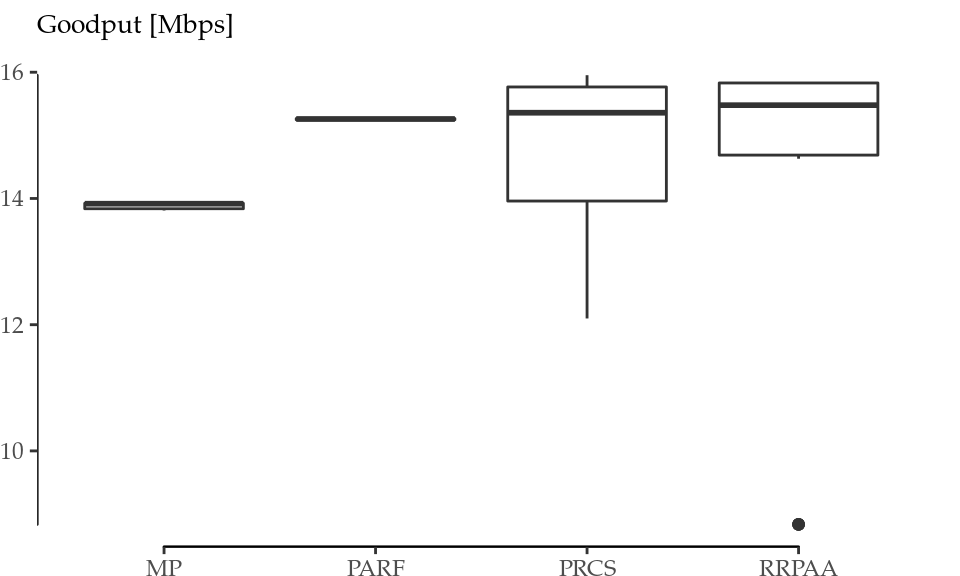
\includegraphics{07-ra-tpc_files/figure-latex/ns3-goodput-1} 

}

\caption[Goodput achieved per simulated algorithm.]{Goodput achieved per simulated algorithm.}\label{fig:ns3-goodput}
\end{marginfigure}

Figure \ref{fig:ns3-efficiency} shows the energy efficiency achieved per
algorithm, computed for all the devices considered. As expected, the
numerical values of the energy efficiency achieved are different across
devices, but the relative performance is essentially the same, as in the
previous case. Indeed, the efficiency follows the pattern seen in Figure
\ref{fig:ns3-goodput}: RRPAA results the most energy efficient in our
scenario, followed by PRCS, PARF and MP. PRCS and RRPAA exhibit the same
variability across replications as in the case of goodput, which is
particularly notable for the most efficient devices, i.e., the HTC
Legend and the Samsung Galaxy Note.




\begin{figure*}

{\centering 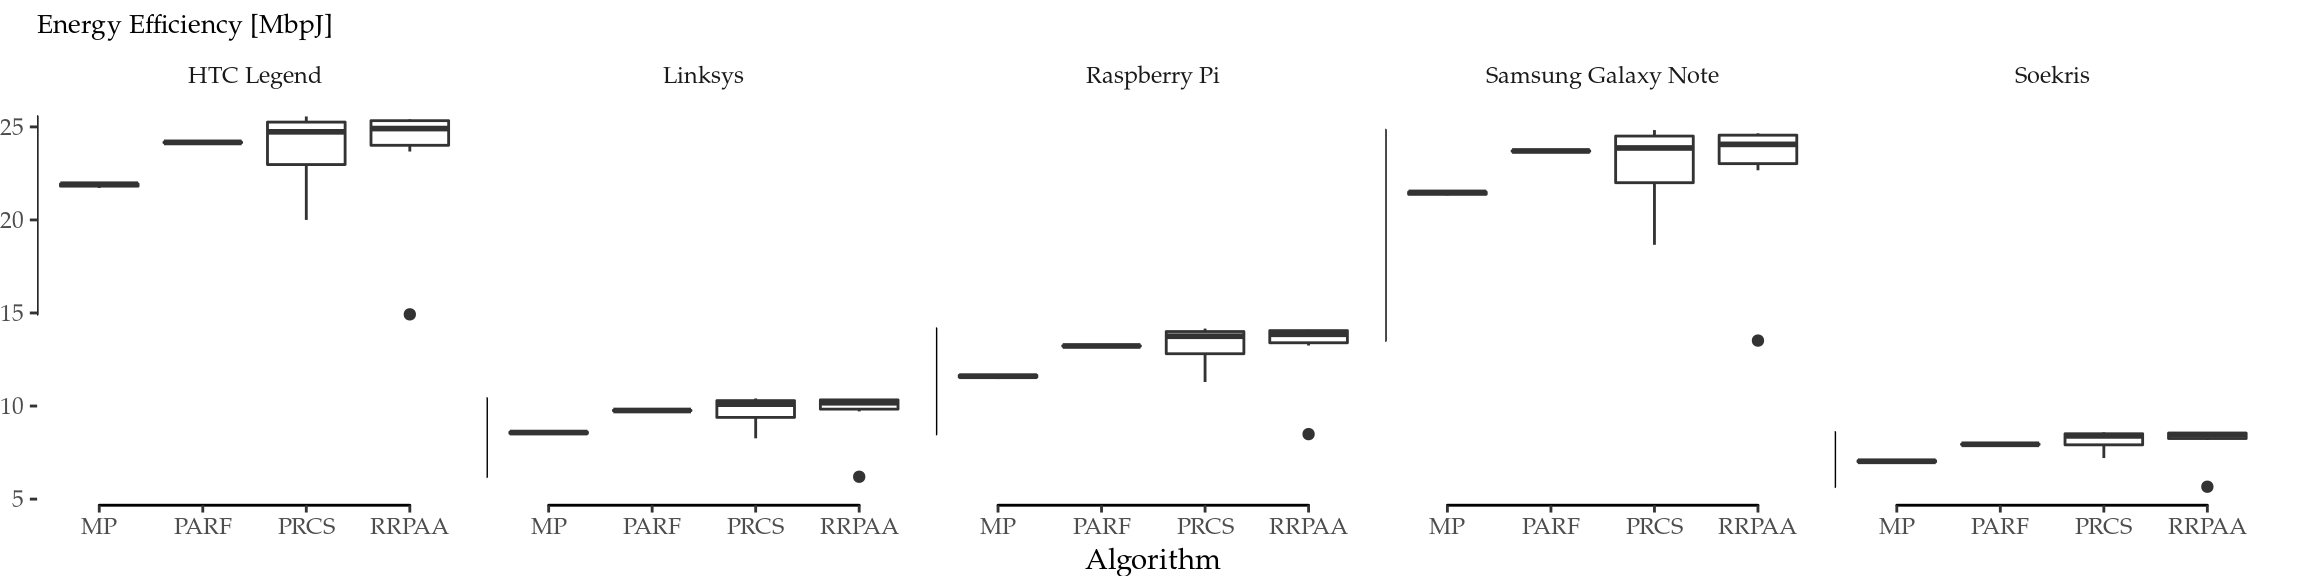
\includegraphics{07-ra-tpc_files/figure-latex/ns3-efficiency-1} 

}

\caption[Energy efficiency achieved per simulated algorithm
and device.]{Energy efficiency achieved per simulated algorithm
and device.}\label{fig:ns3-efficiency}
\end{figure*}

In order to shed some light into the reasons behind the differences in
performance, Figures \ref{fig:ns3-evol} show the behaviour of each
algorithm throughout the simulation time for one run, showing the
evolution of the MCS and TXP chosen by each algorithm, respectively.
Here, we can clearly differentiate that there are two kinds of
behaviour: while MP and PARF are constantly sampling other MCSs and
TXPs, PRCS and RRPAA are much more conservative in that sense, and tend
to keep the same configuration for longer periods of time.




\begin{figure*}

{\centering 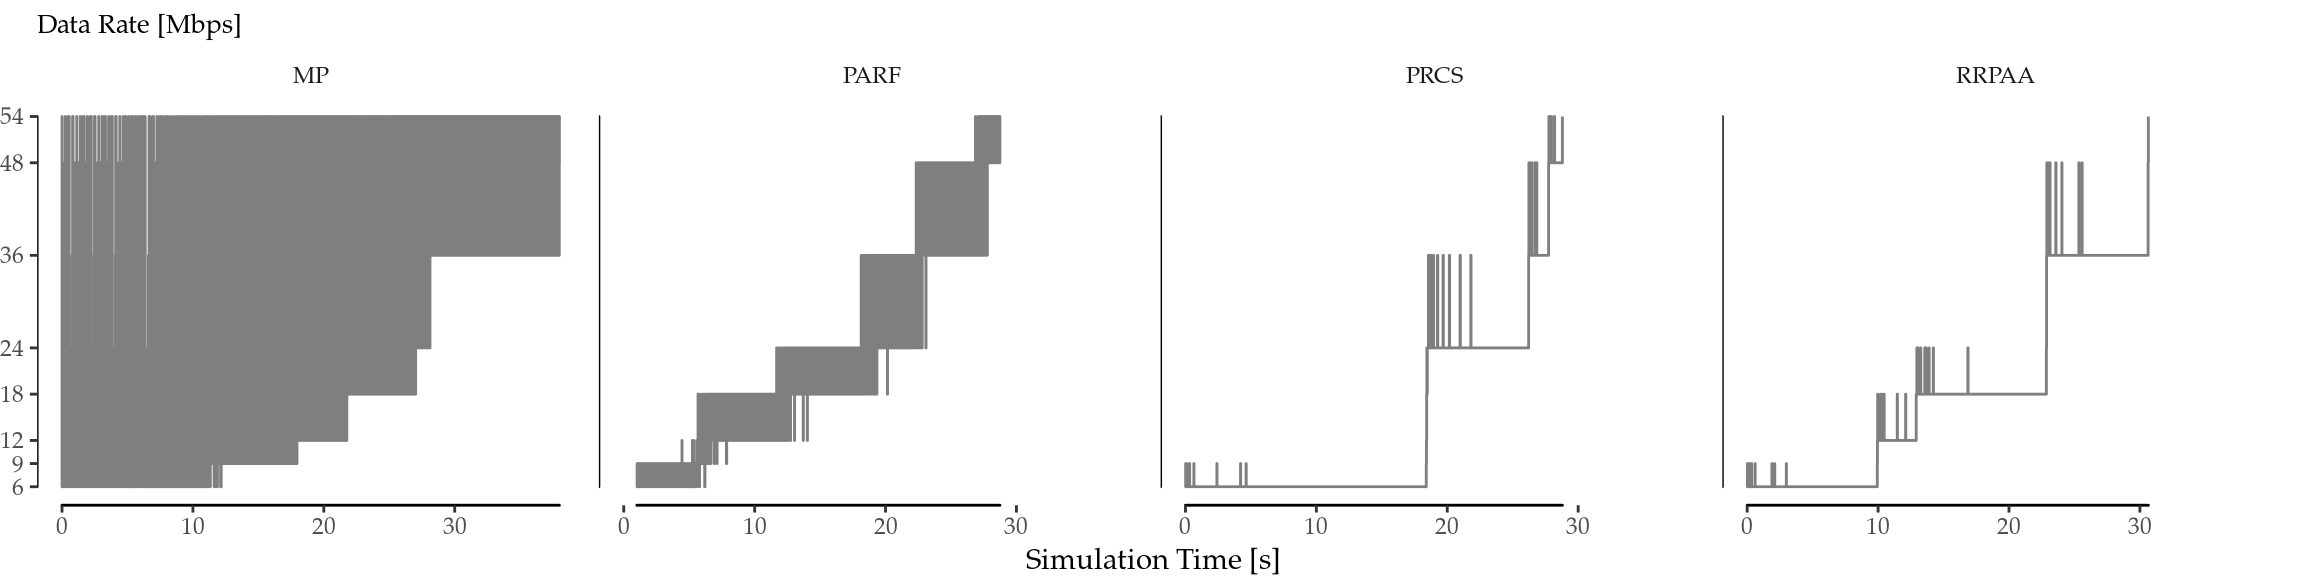
\includegraphics{07-ra-tpc_files/figure-latex/ns3-evol-1} 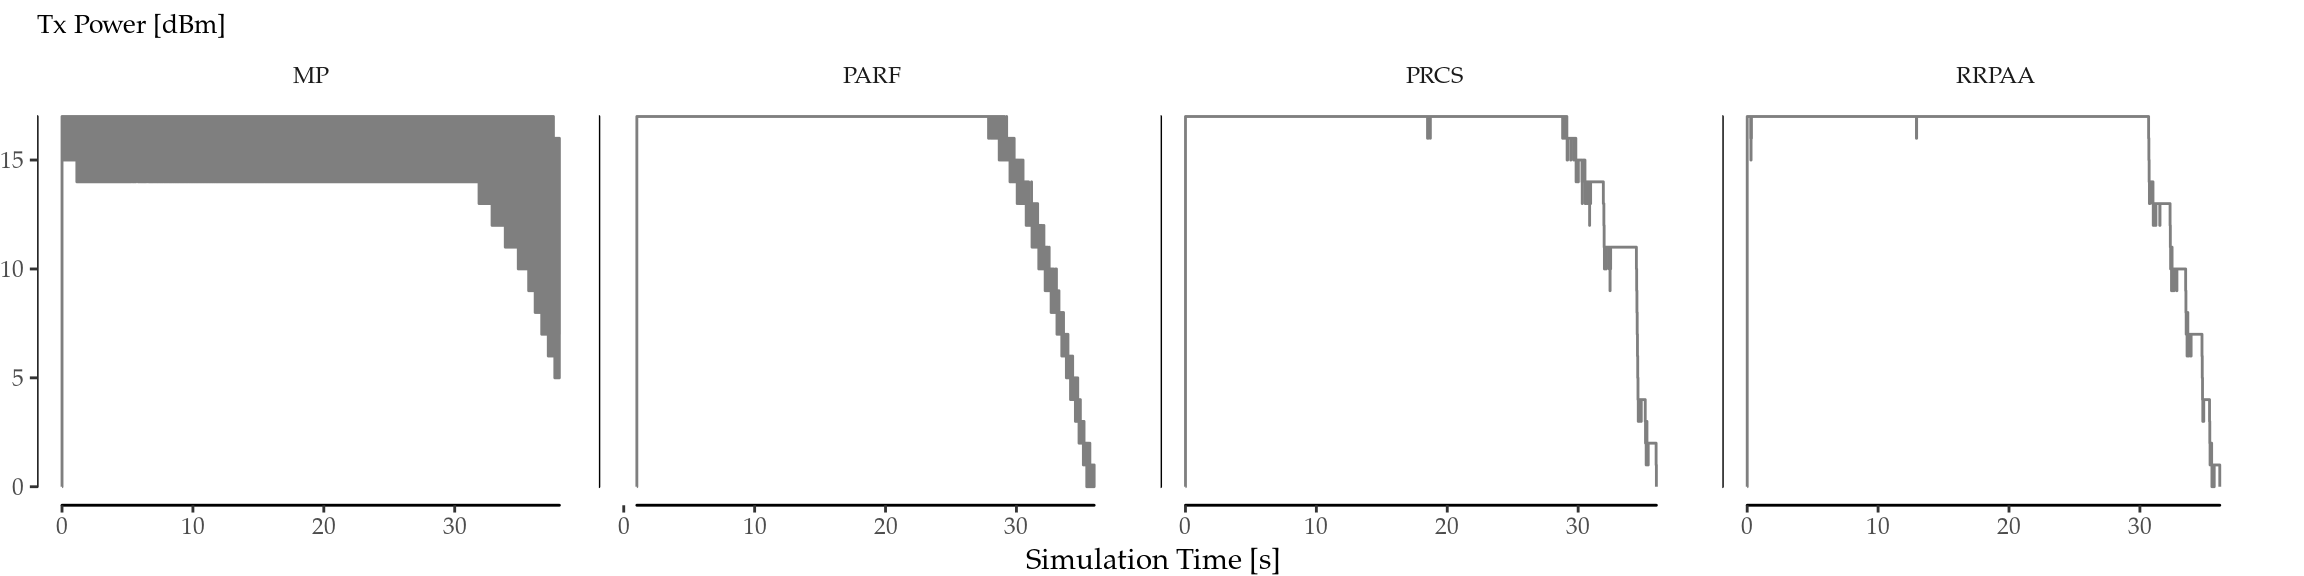
\includegraphics{07-ra-tpc_files/figure-latex/ns3-evol-2} 

}

\caption[MCS (top) and TXP (bottom) evolution per algorithm for a
selected run.]{MCS (top) and TXP (bottom) evolution per algorithm for a
selected run.}\label{fig:ns3-evol}
\end{figure*}

MP randomly explores the whole MCS/TXP space above a basic
\emph{guaranteed} value, and this is the explanation for the apparently
uniformly greyed zone. Also, this aggressive approach is clearly a
disadvantage in the considered toy scenario (deterministic walk,
one-to-one, no obstacles), and this is why the achieved goodput in
Figure \ref{fig:ns3-goodput} is slightly smaller than the one achieved
by the others. PARF, on its part, only explores the immediately higher
MCS/TXP, which leads to a higher goodput and efficiency.

On the other hand, PRCS and RRPAA sampling is much more sparse in time.
As a consequence, Figures \ref{fig:ns3-evol} show more differences
across replications, leading to the high variability shown in Figure
\ref{fig:ns3-goodput} compared to MP and PARF.

In terms of TXP, all the algorithms exhibit a similar
\emph{aggressiveness}, in the sense that they use a high TXP value in
general. Indeed, as Figure \ref{fig:ns3-evol} (bottom) shows, the TXP is
the highest possible until the very end of the simulation, when the STA
is very close to the AP. This is the cause for the high correlation
between Figures \ref{fig:ns3-goodput} and \ref{fig:ns3-efficiency}.

A noteworthy characteristic of PRCS and RRPAA is that, in general, they
\emph{delay} the MCS change decision, as depicted in Figure
\ref{fig:ns3-evol} (top). Most of the times, they do not even use the
whole space of MCS available, unlike MP and PARF. Because of this, they
tend to achieve the best goodput and energy efficiency.

\hypertarget{conservativeness-at-mode-transitions}{%
\section{Conservativeness at Mode
Transitions}\label{conservativeness-at-mode-transitions}}

Building on the concept of \emph{conservativeness} (i.e., the tendency
to select a lower MCS/TXP in the transition regions), we explore whether
there is any correlation with the energy efficiency achieved by a
certain algorithm and this tendency. For that purpose, we first define a
proper metric.

In the first place, we define the \emph{normalised average MCS} as the
area under the curve in Figure \ref{fig:ns3-evol} (top) normalised by
the total simulation time and the maximum MCS:
%
\begin{equation}
 \widehat{\mathrm{MCS}} = \frac{1}{\max(\mathrm{MCS}) \cdot t_\mathrm{sim}}\int_0^{t_\mathrm{sim}} \mathrm{MCS}(t)dt
 \label{eq:MCShat}
\end{equation}
%
where \(t_\mathrm{sim}\) is the simulation time and
\(\max(\mathrm{MCS})\) is 54 Mbps in our case. The same concept can be
applied to the TXP:
%
\begin{equation}
 \widehat{\mathrm{TXP}} = \frac{1}{\max(\mathrm{TXP}) \cdot t_\mathrm{sim}}\int_0^{t_\mathrm{sim}} \mathrm{TXP}(t)dt
 \label{eq:TXPhat}
\end{equation}
%
where \(\max(\mathrm{TXP})\) is 17 dBm in our case. Both
\(\widehat{\mathrm{MCS}}\) and \(\widehat{\mathrm{TXP}}\) are unitless
scores between 0 and 1, and lower values mean a more conservative
algorithm. Therefore, we can define a \emph{Conservativeness Index} (CI)
as the inverse of the product of both scores:
%
\begin{equation}
 \mathrm{CI} = \frac{1}{\widehat{\mathrm{MCS}} \cdot \widehat{\mathrm{TXP}}}
 \label{eq:CI}
\end{equation}
%
where \(\mathrm{CI}>1\).

We computed the CI\footnote{It must be taken into account that the CI is
  not suitable for comparing \emph{any} algorithm. For instance, in an
  extreme case, an ``algorithm'' could select 6 Mbps and 0 dBm always,
  resulting in a very low CI, but a very bad performance at the same
  time. The CI should only be used for comparing similarly performant
  algorithms, as it is the case in our study given the results shown in
  Figures \ref{fig:ns3-goodput} and \ref{fig:ns3-efficiency}.} for each
device and run, and the final results are depicted in Figure
\ref{fig:ns3-conservativeness} as the average CI across different runs
vs.~the median energy efficiency in Figure \ref{fig:ns3-efficiency}.





\begin{figure*}[!b]

{\centering 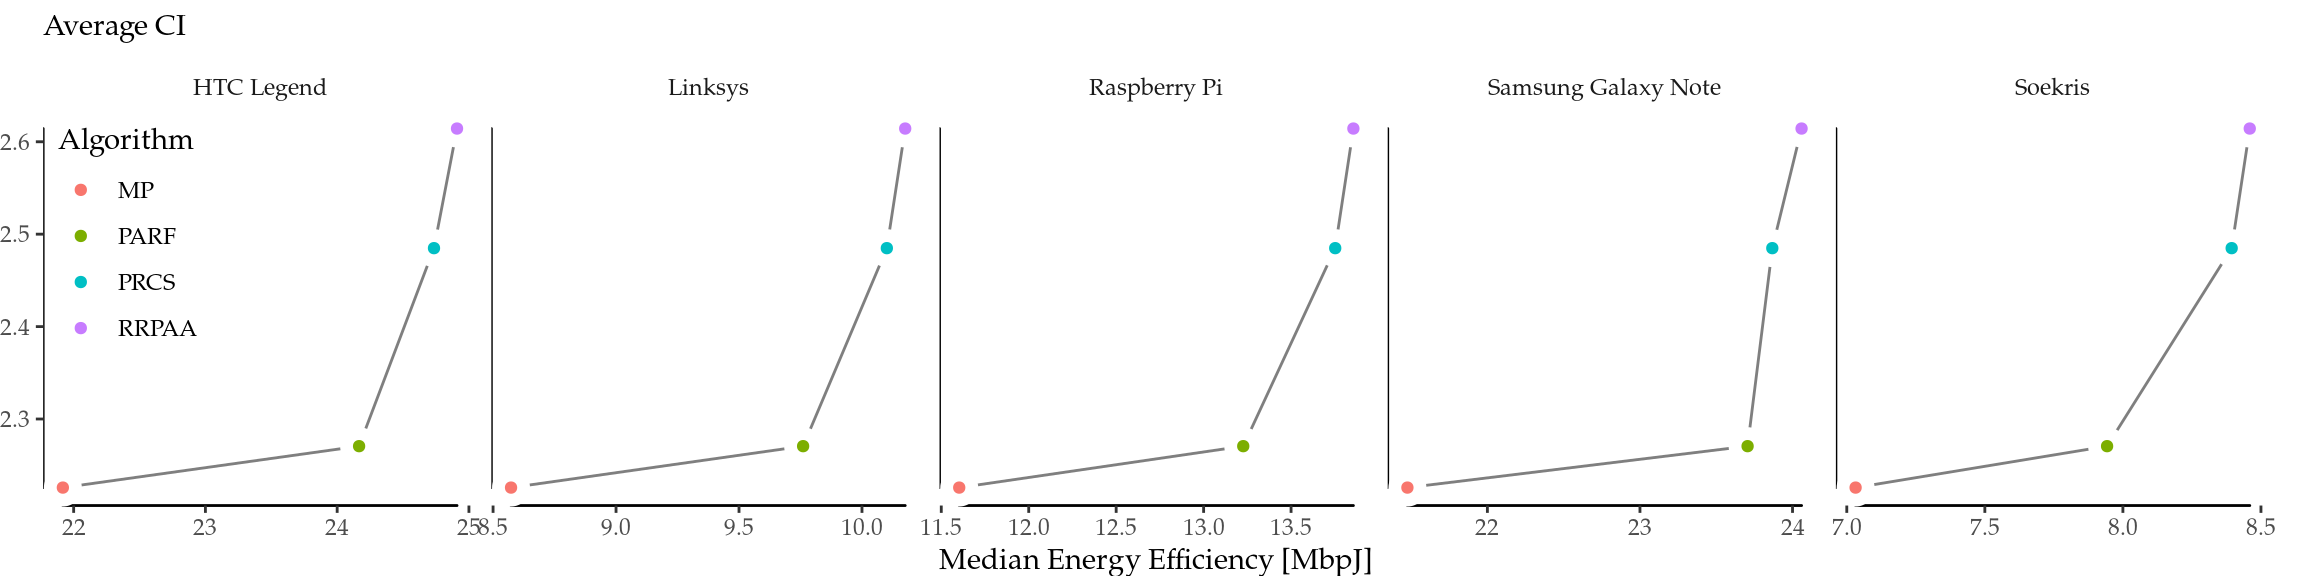
\includegraphics{07-ra-tpc_files/figure-latex/ns3-conservativeness-1} 

}

\caption[Relationship between Conservativeness Index
(tendency to select lower MCS and TXP) and energy effienciency per
simulated device.]{Relationship between Conservativeness Index
(tendency to select lower MCS and TXP) and energy effienciency per
simulated device.}\label{fig:ns3-conservativeness}
\end{figure*}

The results in Figure \ref{fig:ns3-conservativeness} show a positive
non-linear relationship between the CI of an algorithm and the energy
efficiency achieved for all the devices considered. MP is the algorithm
with the lowest CI, which is in consonance with its aggressiveness
(i.e., frequent jumps between MCS/TXP values, as shown in Figures
\ref{fig:ns3-evol}, and the goodput achieved was also the lowest, as
depicted in Figure \ref{fig:ns3-goodput}. On the other hand, PARF, PRCS
and RRPAA achieved a similar performance in terms of goodput, but the
ones with the most conservative behaviour (PRCS and RRPAA, as it can be
seen in Figures \ref{fig:ns3-evol}) also achieve both the highest CI and
energy efficiency.

This result evidences that the performance gaps uncovered by Figure
\ref{fig:efficiency-goodput} under optimal conditions have also an
impact in real-world RA-TPC algorithms. Therefore, we confirm that this
issue must be taken into account in the design of more energy-efficient
rate and transmission power control algorithms.

\hypertarget{summary-4}{%
\section{Summary}\label{summary-4}}

We have
extended\cite[0pt]{contrib-07}\marginnote{\hypersetup{hidelinks}\color{white}\citet{contrib-07}}
our results from Chapter \ref{ch:06} regarding the role of
\emph{conservativeness} at mode transitions in achieving better energy
efficiency in RA-TPC algorithms. We have developed a metric to compare
algorithms, and we have assessed the performance of four
state-of-the-art schemes through simulation. We have demonstrated that
certain conservativeness can resolve the trade-off between throughput
and energy efficiency optimality, thus making a difference for properly
designed energy-aware algorithms.

Further research is needed to develop proper heuristics to leverage
these findings. In particular, the \emph{downwards} direction, as
described in Section \ref{heuristics-for-ra-tpc-algorithms}, is the most
challenging, because it requires predicting the evolution of the channel
state.

\hypertarget{ch:08}{%
\chapter{A Novel Discrete-Event Simulation Framework}\label{ch:08}}

\newthought{Simulation frameworks} are important tools for the analysis
and design of communication networks and protocols, but they can result
extremely costly and/or complex (for the case of very specialised
tools), or too naive and lacking proper features and support (for the
case of ad-hoc tools). Our own research experience in the previous
chapter has pointed us towards the need for new tools sitting between
these two paradigms, supporting the efficient simulation of relatively
complex scenarios at a low implementation cost.

In this chapter, we introduce a recent event-driven simulation package,
\texttt{simmer}, and show its applicability in fast prototyping.
\texttt{simmer} sits between the above two complexity extremes, and
combines a number of features that supports, among others, versatility
and repeatability. More specifically, some of the key advantages of
\texttt{simmer} are as follows:

\begin{itemize}
\tightlist
\item
  It is based on the very popular R programming
  language\cite[0pt]{R-base}\marginnote{\hypersetup{hidelinks}\color{white}\citet{R-base}},
  which benefits from a large community of users and contributors, but
  also natively supports the analysis of results via the many R
  statistical and visualization packages.
\item
  The code has been peer-reviewed, and it is an official
  package\cite[0pt]{R-simmer}\marginnote{\hypersetup{hidelinks}\color{white}\citet{R-simmer}},
  with numerous examples readily available, potentially supported by a
  notable user population.
\item
  In addition to its ease of use and versatility, its code is partially
  optimised for speed, and therefore it can simulate relatively complex
  scenarios under reasonable times.
\end{itemize}

In the following, we first describe the simulation core design and its
architecture. Then we provide a quick overview of \texttt{simmer} and
its key features. Finally, we showcase the versatility of
\texttt{simmer} to easily model a Massive Internet-of-Things (IoT)
scenario where thousands of metering devices share the same channel.
Here, we analyse the impact of access parameters on performance, with a
particular interest in the energy required to deliver the information,
which will ultimately impact the lifetime of devices running on
batteries.

\hypertarget{the-simulation-core-design}{%
\section{The Simulation Core Design}\label{the-simulation-core-design}}

The core of any modern discrete-event simulator comprises two main
components: an event list, ordered by time of occurrence, and an event
loop that extracts and executes events. In contrast to other interpreted
languages such as Python, which is compiled by default to an
intermediate byte-code, R code is purely parsed and evaluated at
runtime\footnote{Some effort has been made in this line with the
  \texttt{compiler} package, introduced in R version 2.13.0
  \citep{R:compiler}, furthermore, a JIT-compiler was included in R
  version 3.4.0.}. This fact makes it a particularly slow language for
Discrete-Event Simulation (DES), which consists of executing complex
routines (pieces of code associated to the events) inside a loop while
constantly allocating and deallocating objects (in the event queue).

In fact, first attempts were made in pure R by these authors, and a
minimal process-based implementation with \texttt{R6}
classes\cite[0pt]{CRAN:R6}\marginnote{\hypersetup{hidelinks}\color{white}\citet{CRAN:R6}}
proved to be unfeasible in terms of performance compared to similar
approaches in pure Python. For this reason, it was decided to provide a
robust and fast simulation core written in C++. The R API interfaces
with this C++ core by leveraging the \texttt{Rcpp}
package\cite[0pt]{Eddelbuettel:2011:Rcpp,Eddelbuettel:2013:Rcpp}\marginnote{\hypersetup{hidelinks}\color{white}\citet{Eddelbuettel:2011:Rcpp,Eddelbuettel:2013:Rcpp}},
which has become one of the most popular ways of extending R packages
with C or C++ code.

The following sections are devoted to describe the simulation core
architecture. First, we establish the DES terminology used in the rest
of the paper. Then, the architectural choices made are discussed, as
well as the event queue and the \emph{simultaneity problem}, an
important topic that every DES framework has to deal with.

\hypertarget{terminology}{%
\subsection{Terminology}\label{terminology}}

This document uses some DES-specific terminology, e.g., \emph{event},
\emph{state}, \emph{entity}, \emph{process} or \emph{attribute}. Such
standard terms can be easily found in any textbook about DES (refer to
\citet{Banks:2005:Discrete}\cite{Banks:2005:Discrete}, for instance).
There are, however, some \texttt{simmer}-specific terms, and some
elements that require further explanation to understand the package
architecture.

\begin{description}
\item[Resource]
A passive entity, as it is commonly understood in standard DES
terminology. However, \texttt{simmer} resources are conceived with
queuing systems in mind, and therefore they comprise two internal
self-managed parts:

\begin{description}
\tightlist
\item[Server]
which, conceptually, represents the resource itself. It has a specified
capacity and can be seized and released.
\item[Queue]
A priority queue of a certain size.
\end{description}
\item[Manager]
An active entity, i.e., a process, that has the ability to adjust
properties of a resource (capacity and queue size) at run-time.
\item[Source]
A process responsible for creating new \emph{arrivals} with a given
interarrival time pattern and inserting them into the simulation model.
\item[Arrival]
A process capable of interacting with resources or other entities of the
simulation model. It may have some attributes and prioritisation values
associated and, in general, a limited lifetime. Upon creation, every
arrival is attached to a given \emph{trajectory}.
\item[Trajectory]
An interlinkage of \emph{activities} constituting a recipe for arrivals
attached to it, i.e., an ordered set of actions that must be executed.
The simulation model is ultimately represented by a set of trajectories.
\item[Activity]
The individual unit of action that allows arrivals to interact with
resources and other entities, perform custom routines while spending
time in the system, move back and forth through the trajectory
dynamically, and much more.
\end{description}

\hypertarget{architecture}{%
\subsection{Architecture}\label{architecture}}

Extending an R package (or any other piece of software written in any
interpreted language) with compiled code poses an important trade-off
between performance and flexibility: placing too much functionality into
the compiled part produces gains in performance, but degrades modelling
capabilities, and vice versa. The following lines are devoted to discuss
how this trade-off is resolved in \texttt{simmer}.

Figure \ref{fig:architecture} sketches a UML (Unified Modelling
Language) description of the architecture, which constitutes a
process-based design, as in many modern DES frameworks. We draw the
attention now to the C++ classes (depicted in white).





\begin{figure}

{\centering 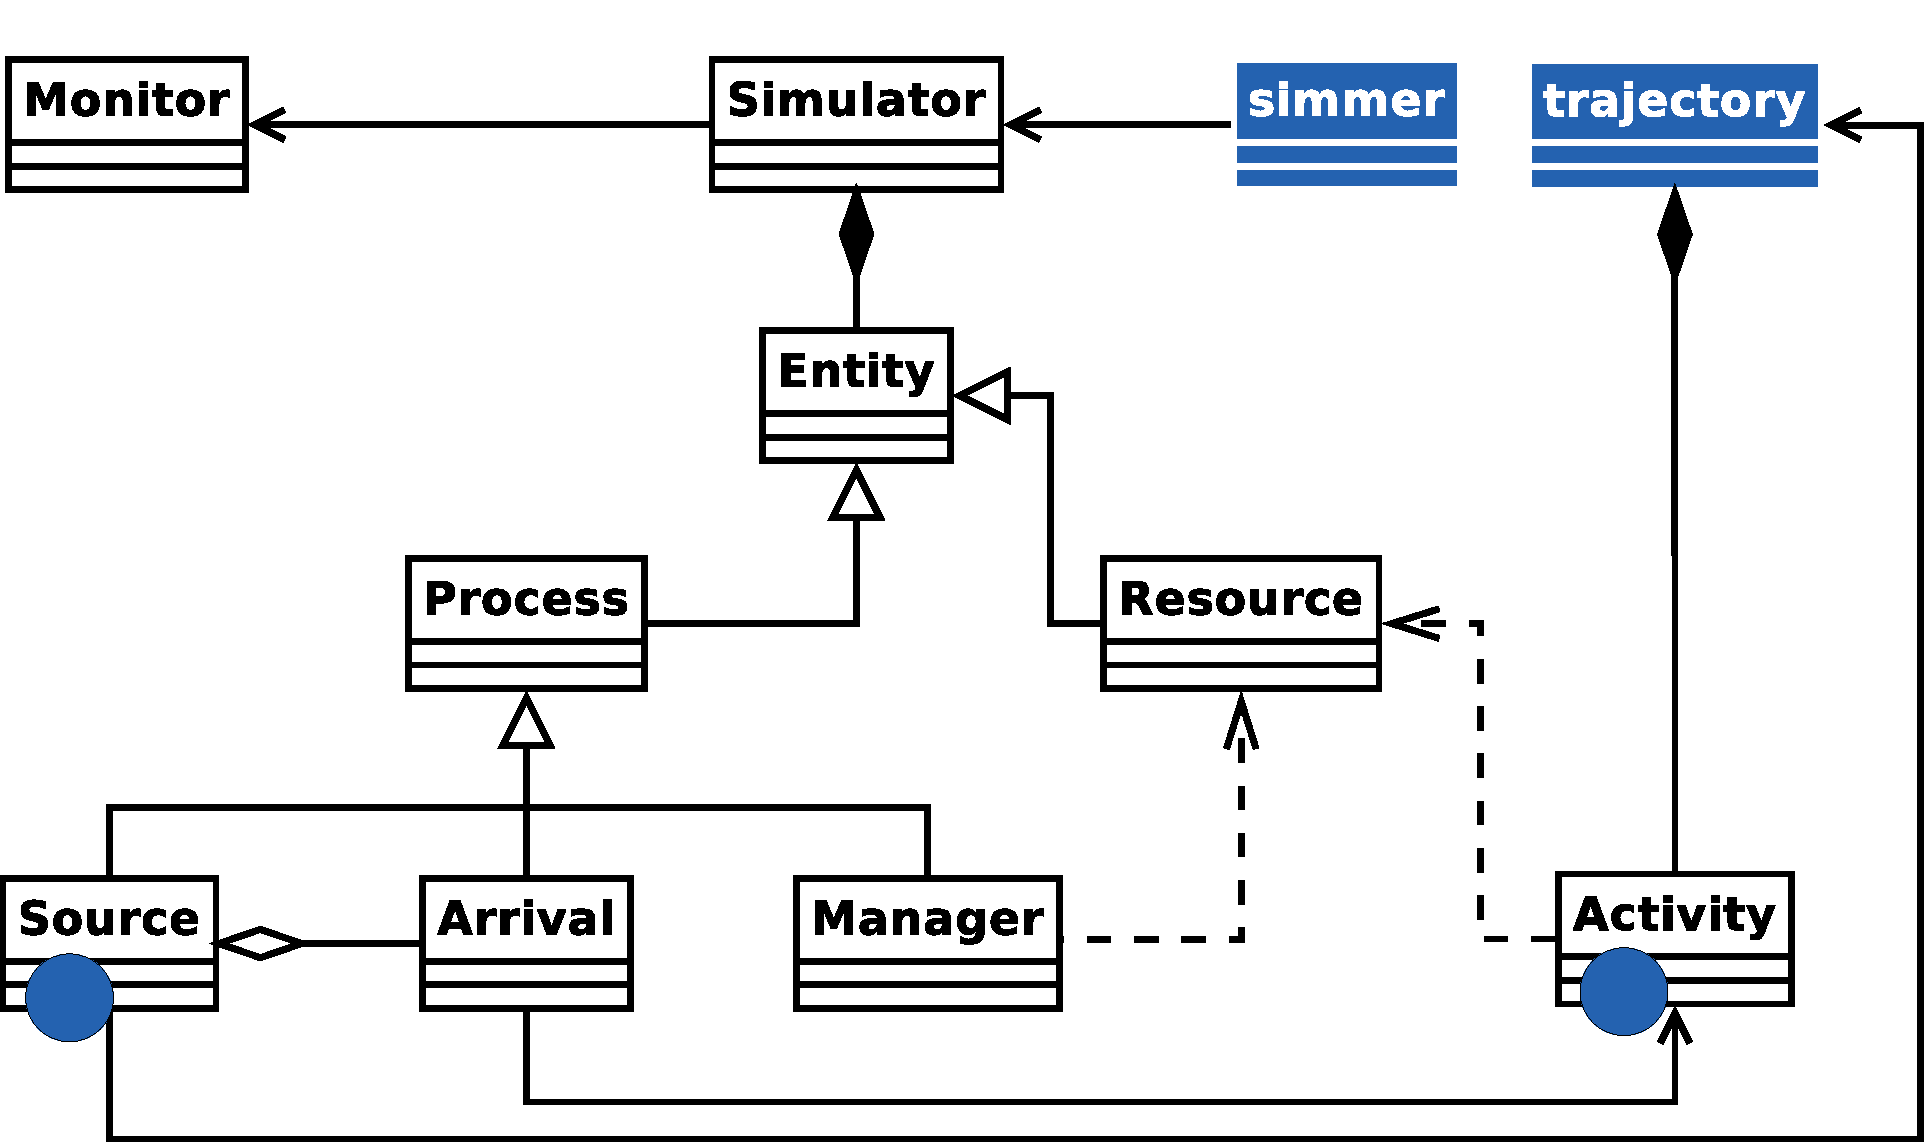
\includegraphics{img/08/jss-simmer-design} 

}

\caption[UML diagram of the simulation core architecture. Blue
classes represent how R encapsulates the C++ core. Blue circles
represent how C++ interfaces with R.]{UML diagram of the simulation core architecture. Blue
classes represent how R encapsulates the C++ core. Blue circles
represent how C++ interfaces with R.}\label{fig:architecture}
\end{figure}

The first main component is the \texttt{Simulator} class. It comprises
the event loop and the event queue, which will be addressed in the next
section. The \texttt{Simulator} provides methods for scheduling and
unscheduling events. Moreover, it is responsible for managing
simulation-wide entities (e.g., resources and arrival sources) and
facilities (e.g., signaling between processes and batches) through
diverse C++ unordered maps:

\begin{itemize}
\tightlist
\item
  Maps of resources and processes (sources, arrivals and managers) by
  name.
\item
  A map of pending events, which allows to unschedule a given process.
\item
  Maps of signals subscribed by arrivals and handlers defined for
  different signals.
\item
  Maps for forming batches of arrivals, named and unnamed.
\end{itemize}

This class also holds global attributes and monitoring information.
Thus, monitoring counters, which are derived from the \texttt{Monitor}
class, are centralised, and they register every change of state produced
during the simulation time. There are five types of built-in changes of
state that are recorded by calling \texttt{Monitor}'s
\texttt{record\_*()} methods:

\begin{itemize}
\tightlist
\item
  An arrival is accepted into a resource (served or enqueued). The
  resource notifies about the new status of its internal counters.
\item
  An arrival leaves a resource. The resource notifies the new status of
  its internal counters, and the arrival notifies start, end and
  activity times in that particular resource.
\item
  A resource is modified during runtime (i.e., a change in the capacity
  or queue size). The resource notifies the new status of its internal
  counters.
\item
  An arrival modifies an attribute, one of its own or a global one. The
  arrival notifies the new value.
\item
  An arrival leaves its trajectory by exhausting the activities
  associated (considered as \emph{finished}) or because of another
  reason (\emph{non-finished}, e.g., it is rejected from a resource).
  The arrival notifies global start, end and activity times.
\end{itemize}

As mentioned in the previous section, there are two types of entities:
passive ones (\texttt{Resource}) and active ones (processes
\texttt{Source}, \texttt{Arrival} and \texttt{Manager}). Sources create
new arrivals, and the latter are the main actors of the simulation
model. Managers can be used for dynamically changing the properties of a
resource (capacity and queue size). All processes share a \texttt{run()}
method that is invoked by the event loop each time a new event is
extracted from the event list.

There is a fourth kind of process not shown in Figure
\ref{fig:architecture}, called \texttt{Task}. It is a generic process
that executes a given function once, and it is used by arrivals,
resources, activities and the simulator itself to trigger dynamic
actions or split up events. A \texttt{Task} is for instance used under
the hood to trigger reneging or to broadcast signals after some delay.

The last main component, completely isolated from the
\texttt{Simulator}, is the \texttt{Activity} class. This abstract class
represents a clonable object, chainable in a double-linked list to form
trajectories. Most of the activities provided by \texttt{simmer} derive
from it. \texttt{Fork} is another abstract class (not depicted in Figure
\ref{fig:architecture}) which is derived from \texttt{Activity}. Any
activity supporting the definition of sub-trajectories must derive from
this one instead, such as \texttt{Seize}, \texttt{Branch} or
\texttt{Clone}. All the activities must implement the virtual methods
\texttt{print()} and \texttt{run()}.

Finally, it is worth mentioning the couple of blue circles depicted in
Figure \ref{fig:architecture}. They represent the \emph{points of
presence} of R in the C++ core, i.e., where the core interfaces back
with R to execute custom user-defined code.

In summary, the C++ core is responsible for all the heavy tasks, i.e.,
managing the event loop, the event list, generic resources and
processes, collecting all the statistics, and so on. And still, it
provides enough flexibility to the user for modelling the interarrival
times from R and execute any custom user-defined code through the
activities.

\hypertarget{the-event-queue}{%
\subsection{The Event Queue}\label{the-event-queue}}

The event queue is the most fundamental part of any DES software. It is
responsible for maintaining a list of events to be executed by the event
loop in an ordered fashion by time of occurrence. This last requirement
establishes the need for a data structure with a low access, search,
insertion and deletion complexity. A binary tree is a well-known data
structure that satisfies these properties, and it is commonly used for
this purpose. Unfortunately, binary trees, or equivalent structures,
cannot be efficiently implemented without pointers, and this is the main
reason why pure R is very inefficient for DES.

In \texttt{simmer}, the event queue is defined as a C++ multiset, a kind
of associative container implemented as a balanced tree internally.
Apart from the efficiency, it was selected to support event unscheduling
through iterators. Each event holds a pointer to a process, which will
be retrieved and run in the event loop. Events are inserted in the event
queue ordered by 1) time of occurrence and 2) priority. This secondary
order criterion is devoted to solve a common issue for DES software
called \emph{the simultaneity problem}.

\hypertarget{the-simultaneity-problem}{%
\paragraph{The Simultaneity Problem}\label{the-simultaneity-problem}}
\addcontentsline{toc}{paragraph}{The Simultaneity Problem}

As noted by \citet{Ronngren:1999:EOP:301429.301456} and
\citet{Jha:2000:SEL:361026.361032}\cite{Ronngren:1999:EOP:301429.301456, Jha:2000:SEL:361026.361032},
there are many circumstances from which simultaneous events (i.e.,
events with the same timestamp) may arise. How they are handled by a DES
framework has critical implications on reproducibility and simulation
correctness.

As an example of the implications, let us consider an arrival seizing a
resource at time \(t_{i-1}\), which has \texttt{capacity=1} and
\texttt{queue\_size=0}. At time \(t_{i}\), two simultaneous events
happen: 1) the resource is released, and 2) another arrival tries to
seize the resource. It is indisputable what should happen in this
situation: the new arrival seizes the resource while the other continues
its path. But note that if 2) is executed \emph{before} 1), the new
arrival is rejected (!). Therefore, it is obvious that release events
must always be executed \emph{before} seize events.

If we consider a dynamically managed resource (i.e., its capacity
changes over time) and, instead of the event 1) in the previous example,
the manager increases the capacity of the resource, we are in the very
same situation. Again, it is obvious that resource managers must be
executed \emph{before} seize attempts.

A further analysis reveals that, in order to preserve correctness and
prevent a simulation crash, it is necessary to break down resource
releases in two parts with different priorities: the release in itself
and a post-release event that tries to serve another arrival from the
queue. Thus, every resource manager must be executed \emph{after}
releases and \emph{before} post-releases. This and other issues are
solved with a priority system (see Table \ref{tab:priorities}) embedded
in the event list implementation that provides a deterministic and
consistent execution of simultaneous events.

\begin{table}

\begin{center}
\resizebox{\linewidth}{!}{
\begin{tabular}{>{\ttfamily}ll}
\toprule
Priority & Event\\
\midrule
MAX & Terminate arrivals\\
RELEASE & Resource release\\
MANAGER & Manager action (e.g., resource capacity change)\\
RELEASE\_POST & Resource post-release (i.e., serve from the queue)\\
... & General activities\\
\addlinespace
MIN & Other tasks (e.g., new arrivals, timers...)\\
\bottomrule
\end{tabular}}
\end{center}
\caption{\label{tab:priorities}Priority system (in decreasing order) and events associated.}
\end{table}

\hypertarget{a-brief-introduction-to-simmer}{%
\section{\texorpdfstring{A Brief Introduction to
\texttt{simmer}}{A Brief Introduction to simmer}}\label{a-brief-introduction-to-simmer}}

Note that \texttt{simmer} does not aim at substituting NS-3 or OMNeT++,
which are the \emph{de facto} standards for open-source network
simulations. Instead, \texttt{simmer} is designed as a general-purpose
DES framework with a human-friendly syntax, and a very gentle learning
curve. It can be used to complement other field-specific simulators as a
rapid prototyping tool that enable insightful analysis of different
designs. As we will illustrate in the next section, with \texttt{simmer}
it is simple to simulate relatively complex scenarios, with the added
benefit of the availability of many convenient data analysis and
representation packages, thanks to the use of R.

The R application programming interface (API) exposed by \texttt{simmer}
revolves around the concept of \emph{trajectory}, which defines the
``path'' in the simulation for entities of the same type. A trajectory
is a recipe for the arrivals attached to it, an ordered set of actions
(or \emph{verbs}) chained together with the pipe
operator\cite[0pt]{CRAN:magrittr}\marginnote{\hypersetup{hidelinks}\color{white}\citet{CRAN:magrittr}}
(\texttt{\%\textgreater{}\%}, whose behaviour is similar to the
command-line pipe). The following example illustrates a basic
\texttt{simmer} workflow, modeling the classical case of customers being
attended by a single clerk with infinite waiting space in a few lines of
code:

\begin{Shaded}
\begin{Highlighting}[]
\KeywordTok{library}\NormalTok{(simmer)}

\NormalTok{cust <-}\StringTok{ }\KeywordTok{trajectory}\NormalTok{(}\StringTok{"customer"}\NormalTok{) }\OperatorTok
\StringTok{  }\KeywordTok{seize}\NormalTok{(}\StringTok{"clerk"}\NormalTok{, }\DataTypeTok{amount=}\DecValTok{1}\NormalTok{) }\OperatorTok
\StringTok{  }\KeywordTok{timeout}\NormalTok{(}\ControlFlowTok{function}\NormalTok{() }\KeywordTok{rexp}\NormalTok{(}\DecValTok{1}\NormalTok{, }\DecValTok{2}\NormalTok{)) }\OperatorTok
\StringTok{  }\KeywordTok{release}\NormalTok{(}\StringTok{"clerk"}\NormalTok{, }\DataTypeTok{amount=}\DecValTok{1}\NormalTok{)}

\NormalTok{env <-}\StringTok{ }\KeywordTok{simmer}\NormalTok{(}\StringTok{"bank"}\NormalTok{) }\OperatorTok
\StringTok{  }\KeywordTok{add_resource}\NormalTok{(}\StringTok{"clerk"}\NormalTok{, }\DataTypeTok{capacity=}\DecValTok{1}\NormalTok{, }\DataTypeTok{queue_size=}\OtherTok{Inf}\NormalTok{) }\OperatorTok
\StringTok{  }\KeywordTok{add_generator}\NormalTok{(}\StringTok{"cust"}\NormalTok{, cust, }\ControlFlowTok{function}\NormalTok{() }\KeywordTok{rexp}\NormalTok{(}\DecValTok{1}\NormalTok{, }\DecValTok{1}\NormalTok{)) }\OperatorTok
\StringTok{  }\KeywordTok{run}\NormalTok{(}\DataTypeTok{until=}\DecValTok{1000}\NormalTok{)}

\NormalTok{arrivals  <-}\StringTok{ }\KeywordTok{get_mon_arrivals}\NormalTok{(env)}
\NormalTok{resources <-}\StringTok{ }\KeywordTok{get_mon_resources}\NormalTok{(env)}
\end{Highlighting}
\end{Shaded}

Given that both the time at the clerk and between customers are
exponential random variables, and the infinite queue length, this
example corresponds, in Kendall's notation, to an M/M/1 queue. It serves
to illustrate the two main elements of \texttt{simmer}: the
\texttt{trajectory} object and the \texttt{simmer} environment (or
\emph{simulation environment}).

The \texttt{customer} trajectory defines the behaviour of a generic
customer: seize a clerk, spend some time, and release it. The
\texttt{env} simulation environment is then defined as one clerk with
infinite queue size and a generator of customers, each one following the
trajectory defined above. Based on this syntax, the flexibility is
provided through a rich set of activities\footnote{See
  \url{https://r-simmer.org/reference/}.} that can be appended to
trajectories, which support: changing arrivals' properties (attributes,
priority, batches), different interactions with the resources (select,
seize, release, change their properties), and the generators (activate,
deactivate, change their properties), and even the definition of
branches (simple, depending on a condition, or parallel) and loops.
Finally, some support to asynchronous programming is also provided
(subscription to signals and registration of handlers).

Not only \texttt{simmer} provides a powerful yet simple syntax, but it
is also \emph{fast}, for example, faster than equivalent frameworks such
as
SimPy\cite[0pt]{SimPy}\marginnote{\hypersetup{hidelinks}\color{white}\citet{SimPy}}
and
SimJulia\cite[0pt]{GitHub:SimJulia}\marginnote{\hypersetup{hidelinks}\color{white}\citet{GitHub:SimJulia}}
for the Python and Julia languages respectively\footnote{See Appendix
  \ref{performance-evaluation-of-simmer} for a complete performance
  evaluation.}. Furthermore, and perhaps more importantly,
\texttt{simmer} implements automatic monitoring capabilities: every
event is accounted for by default, both for arrivals (starting and
ending times, activity time, ending condition, resources traversed) and
resources (server and queue status), and all this information can be
easily retrieved in standard R data frames for further processing of
results (last two lines of the \emph{clerk} example).

\hypertarget{use-case-energy-efficiency-for-massive-iot}{%
\section{Use case: Energy Efficiency for Massive
IoT}\label{use-case-energy-efficiency-for-massive-iot}}

We consider the case of a massive Internet-of-Things (mIoT) scenario, a
use case for Long Term Evolution (LTE) and next-generation 5G networks,
as defined by the
3GPP\cite[0pt]{miot}\marginnote{\hypersetup{hidelinks}\color{white}\citet{miot}}.
As Figure \ref{fig:scenario3def} (left) illustrates, we consider a
single LTE macrocell in a dense urban area. The buildings in the cell
area are populated with \(N\) smart meters (for electricity, gas, and
water), and each meter operates independently as a Narrowband IoT
(NB-IoT) device.



\begin{figure*}

{\centering 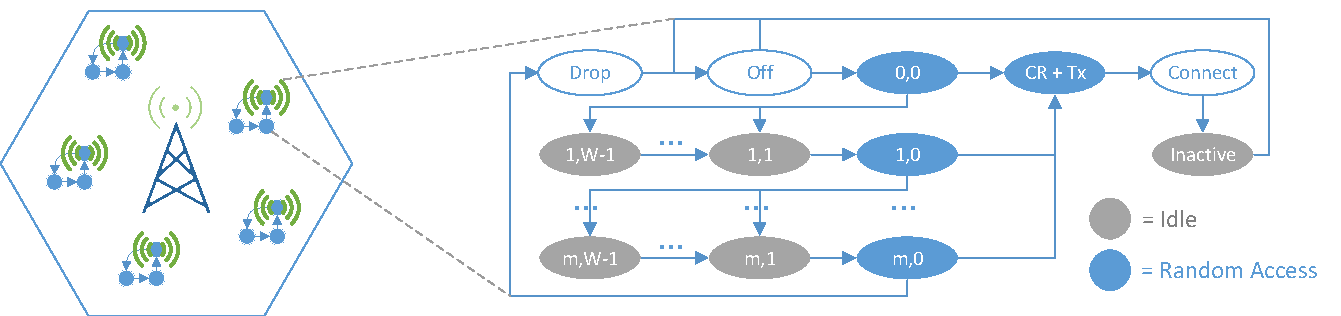
\includegraphics{img/08/scenario} 

}

\caption[Description of the simulation scenario.]{Description of the simulation scenario.}\label{fig:scenario3def}
\end{figure*}

The devices' behaviour is modeled following the diagram depicted in
Figure \ref{fig:scenario3def} (right), which is a simplified version of
the Markov chain model developed in \citet[Figure
5]{iotModel}\cite{iotModel}. A device may stay in \texttt{RRC\ Idle}
(`Off'), and awakes with some periodicity to upload its reading. This
communication phase encompasses a contention-based random access (RA)
procedure, with a backoff time randomly chosen between \((0,W)\) time
slots, and up to \(m\) retransmissions. If the connection request fails,
the reading is dropped, and the device returns to the `Off' state. If
the connection is successful, we assume that the device implements the
Control Plane Cellular IoT (CP) optimization (see \citet{iotModel}), so
that the data is transmitted over the \texttt{RRC\ Connection} request
phase using the Non Access Stratum (NAS) level. Then, the device has to
wait (`Inactive') until the connection is released, and eventually
returns to the `Off' state.

The goal of this use case is to study the effect of synchronization
across IoT devices (for instance, due to a power outage) in the energy
consumption. As in \citet{iotCollision}\cite{iotCollision}, we assume
that a device provides its readings as often as every hour, and the
cases of \(N=\{5, 10, 30\} \cdot 10^3\) devices in one cell are
considered. In order to study different levels of synchronization, each
node implements an additional backoff window prior to the RA procedure.
Furthermore, we selected \(m=9\) and \(W=20\); the rest of the
parameters (power consumption, timings, message sizes\ldots{}) can be
found in \citet[Table I]{iotModel}.

\hypertarget{implementation-details}{%
\paragraph{Implementation Details}\label{implementation-details}}
\addcontentsline{toc}{paragraph}{Implementation Details}

This scenario requires a single \texttt{meter} trajectory implementing
the logic of each IoT device in an infinite loop, and \(N\) workers are
attached to it at \(t=0\).

\begin{Shaded}
\begin{Highlighting}[]
\CommentTok{# IoT device logic}
\NormalTok{meter <-}\StringTok{ }\KeywordTok{trajectory}\NormalTok{() }\OperatorTok
\StringTok{  }\KeywordTok{trap}\NormalTok{(}\StringTok{"reading"}\NormalTok{) }\OperatorTok
\StringTok{  }\CommentTok{# sleep}
\StringTok{  }\KeywordTok{set_attribute}\NormalTok{(}\StringTok{"P"}\NormalTok{, }\DecValTok{0}\NormalTok{) }\OperatorTok
\StringTok{  }\KeywordTok{wait}\NormalTok{() }\OperatorTok
\StringTok{  }\KeywordTok{timeout}\NormalTok{(}\ControlFlowTok{function}\NormalTok{() }\KeywordTok{round}\NormalTok{(}\KeywordTok{runif}\NormalTok{(}\DecValTok{1}\NormalTok{, }\DecValTok{0}\NormalTok{, param[[}\StringTok{"backoff"}\NormalTok{]]), }\DecValTok{3}\NormalTok{)) }\OperatorTok
\StringTok{  }\CommentTok{# ra start}
\StringTok{  }\NormalTok{simmer}\OperatorTok{::}\KeywordTok{select}\NormalTok{(preambles, }\DataTypeTok{policy=}\StringTok{"random"}\NormalTok{) }\OperatorTok
\StringTok{  }\KeywordTok{seize_selected}\NormalTok{(}
    \DataTypeTok{continue=}\KeywordTok{c}\NormalTok{(}\OtherTok{TRUE}\NormalTok{, }\OtherTok{TRUE}\NormalTok{),}
    \CommentTok{# ra & tx}
    \DataTypeTok{post.seize=}\KeywordTok{trajectory}\NormalTok{() }\OperatorTok
\StringTok{      }\KeywordTok{set_attribute}\NormalTok{(}\StringTok{"P"}\NormalTok{, Pra) }\OperatorTok
\StringTok{      }\KeywordTok{timeout}\NormalTok{(Tra) }\OperatorTok
\StringTok{      }\KeywordTok{release_selected}\NormalTok{() }\OperatorTok
\StringTok{      }\KeywordTok{set_attribute}\NormalTok{(}\StringTok{"P"}\NormalTok{, Ptx) }\OperatorTok
\StringTok{      }\KeywordTok{timeout}\NormalTok{(Ttx),}
    \CommentTok{# ra & backoff & retry}
    \DataTypeTok{reject=}\KeywordTok{trajectory}\NormalTok{() }\OperatorTok
\StringTok{      }\KeywordTok{set_attribute}\NormalTok{(}\StringTok{"P"}\NormalTok{, Pra) }\OperatorTok
\StringTok{      }\KeywordTok{timeout}\NormalTok{(Tra) }\OperatorTok
\StringTok{      }\KeywordTok{set_attribute}\NormalTok{(}\StringTok{"P"}\NormalTok{, Pi) }\OperatorTok
\StringTok{      }\KeywordTok{timeout}\NormalTok{(}\ControlFlowTok{function}\NormalTok{() }\KeywordTok{sample}\NormalTok{(}\DecValTok{1}\OperatorTok{:}\DecValTok{20}\NormalTok{, }\DecValTok{1}\NormalTok{) }\OperatorTok{*}\StringTok{ }\FloatTok{1e-3}\NormalTok{) }\OperatorTok
\StringTok{      }\KeywordTok{rollback}\NormalTok{(}\DecValTok{6}\NormalTok{, }\DataTypeTok{times=}\NormalTok{m)}
\NormalTok{  ) }\OperatorTok
\StringTok{  }\KeywordTok{rollback}\NormalTok{(}\DecValTok{5}\NormalTok{, }\DataTypeTok{times=}\OtherTok{Inf}\NormalTok{)}
\end{Highlighting}
\end{Shaded}

Each device registers itself for a given signal (``reading''), and waits
in sleep mode until a new reading is requested, which is triggered by a
secondary trajectory (\texttt{trigger}).

\begin{Shaded}
\begin{Highlighting}[]
\CommentTok{# trigger a reading for all the meters every tx_period}
\NormalTok{trigger <-}\StringTok{ }\KeywordTok{trajectory}\NormalTok{() }\OperatorTok
\StringTok{  }\KeywordTok{timeout}\NormalTok{(tx_period) }\OperatorTok
\StringTok{  }\KeywordTok{send}\NormalTok{(}\StringTok{"reading"}\NormalTok{) }\OperatorTok
\StringTok{  }\KeywordTok{rollback}\NormalTok{(}\DecValTok{2}\NormalTok{, }\DataTypeTok{times=}\OtherTok{Inf}\NormalTok{)}
\end{Highlighting}
\end{Shaded}

As soon as a new reading is signalled, the RA procedure starts by
randomly selecting one of the 54 preambles available, which are defined
as resources. The process of seizing a preamble encompasses two
sub-trajectories:

\begin{itemize}
\tightlist
\item
  If there are no collisions, the preamble is successfully seized, and
  the \texttt{post.seize} sub-trajectory is executed, which transmits a
  reading.
\item
  If there is collision, rejection occurs, and the \texttt{reject}
  sub-trajectory is executed, which performs the RA backoff (for a
  random number of slots), and restarts the RA procedure (for a maximum
  of \(m\) retries).
\end{itemize}

Both sub-trajectories set the appropriate power levels \(P\) for the
appropriate amount of time. In this case, these power levels throughout
the simulation time are retrieved with the
\texttt{get\_mon\_attributes()} method. The energy is concisely computed
and represented using the packages
\texttt{dplyr}\cite[0pt]{CRAN:dplyr}\marginnote{\hypersetup{hidelinks}\color{white}\citet{CRAN:dplyr}}
and
\texttt{ggplot}\cite[0pt]{CRAN:ggplot2}\marginnote{\hypersetup{hidelinks}\color{white}\citet{CRAN:ggplot2}}.




\begin{figure}

{\centering 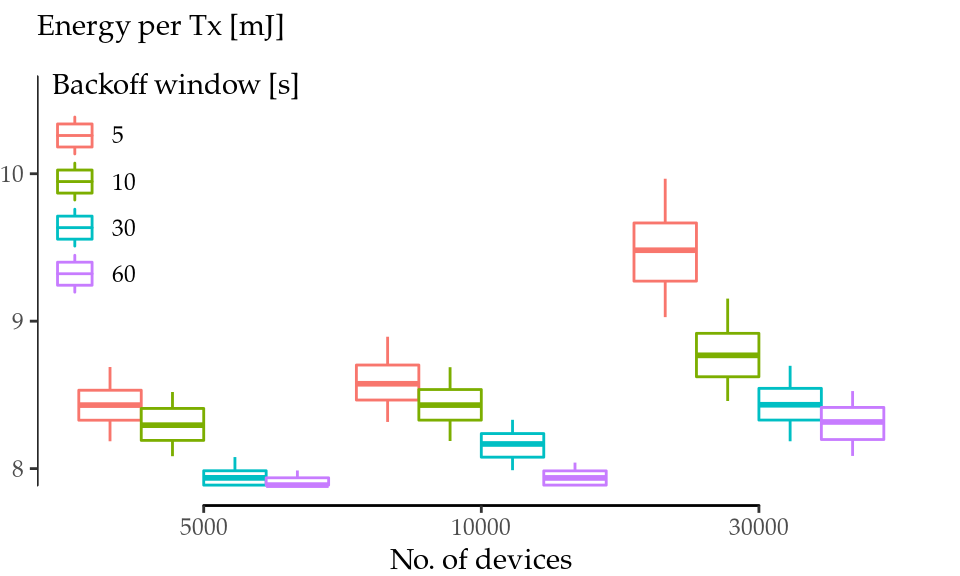
\includegraphics{08-simmer_files/figure-latex/iot-energy-1} 

}

\caption[Energy consumption per transmission attempt for
different traffic models and number of devices.]{Energy consumption per transmission attempt for
different traffic models and number of devices.}\label{fig:iot-energy}
\end{figure}

Figure \ref{fig:iot-energy} shows the results for one simulated day. It
depicts the energy consumed per reading considering a uniform backoff
window between 0 and 5 (\emph{highly synchronised}), 10, 30, and 60
seconds (\emph{non-synchronised}). As the number of devices and the
level of synchronization grow, the random-access opportunities (RAOs)
per second grow as well producing more and more collisions. These
collisions cause retries, and a noticeable impact in the energy
consumption (up to 12\% more energy per reading). Therefore, this use
case shows the paramount importance of randomizing node activation in
mIoT scenarios in order to avoid RAO peaks and a premature battery
drain.

\begin{margintable}[-20mm]

\begin{center}
\begin{tabular}{lr}
\toprule
  & Features\\
\midrule
Simulation time (s) & 150\\
No. of parallel scenarios & 12\\
Max. events, 1 scenario & 28364172\\
Total no. of events & 98952165\\
Implementation lines & 42\\
\addlinespace
Analysis + plotting lines & 14\\
\bottomrule
\end{tabular}
\end{center}
\caption{\label{tab:simulation-overview}Overview of simulation features.}
\end{margintable}

\newthought{The simulation} was run with a machine equipped with an
Intel(R) Xeon(R) CPU E5-2620 v4 @ 2.10GHz x4 (32 cores), and 64 GB of
RAM, Debian GNU/Linux 8, R 3.3.2, and \texttt{simmer} 3.6. Table
summarises the main simulation statistics for this scenario. These
numbers attest that \texttt{simmer} can be used to simulate relatively
complex scenarios with very few lines of code\footnote{The full code is
  available online at
  \url{https://r-simmer.org/articles/simmer-aa-5g\#energy-efficiency-for-massive-iot}.}.

\hypertarget{summary-5}{%
\section{Summary}\label{summary-5}}

The \texttt{simmer} package presented in this
chapter\cite[0pt]{contrib-08a}\marginnote{\hypersetup{hidelinks}\color{white}\citet{contrib-08a}}
brings a generic yet powerful process-oriented Discrete-Event Simulation
framework to R. \texttt{simmer} combines a robust and fast simulation
core written in C++ with a rich and flexible R API. The main modelling
component is the \emph{activity}. Activities are chained together with
the pipe operator into \emph{trajectories}, which are common paths for
processes of the same type. \texttt{simmer} provides a broad set of
activities, and allows the user to extend their capabilities with custom
R functions.

Monitoring is automatically performed by the underlying simulation core,
thereby enabling the user to focus on problem modelling. \texttt{simmer}
enables simple replication and parallelisation with standard R tools.
Data can be extracted into R data frames from a single simulation
environment or a list of environments, each of which is marked as a
different replication for further analysis.

We have
demonstrated\cite[0pt]{contrib-08b}\marginnote{\hypersetup{hidelinks}\color{white}\citet{contrib-08b}}
the usability and suitability of \texttt{simmer} for fast prototyping of
a 5G-inspired scenario. The code developed highlights some of the
characteristics that make \texttt{simmer} attractive for researchers and
practitioners in communications research.

\begin{itemize}
\tightlist
\item
  A novel and intuitive trajectory-based approach that simplifies the
  simulation of large networks of queues, including those with feedback.
\item
  Flexible resources, with dynamic capacity and queue size, priority
  queueing and preemption.
\item
  Flexible generators of arrivals that can draw interarrival times from
  any theoretical or empirical distribution via a function call.
\item
  Asynchronous programming features and monitoring capabilities, which
  helps the researcher focus into the model design.
\end{itemize}

It is likewise remarkable the ease with which multiple scenarios, with
different parameters, can be simulated concurrently thanks to base R
functions. Thus, exploring a large number of combinations of parameter
values is not only straightforward, but also as fast as the slowest
thread given enough number of CPU cores available.

\bookmarksetup{startatroot}
\addtocontents{toc}{\partseparator}

\hypertarget{ch:09}{%
\chapter{Conclusions and Future Work}\label{ch:09}}

\newthought{This thesis} has been devoted to the study of the energy
efficiency of mobile user devices at multiple layers by means of
experimentation, mathematical modelling and simulation. Although the
latter two methods are important tools for science in general, and for
this field in particular, we must emphasise the complexity and paramount
importance of experimentation.

\newthought{In a preeminent experimental part} that has served as a
basis for the rest of the thesis, we have assembled a comprehensive
energy measurement framework, and a robust methodology, which is capable
of measuring a wide range of wireless devices, as well as individual
components, with high accuracy and precision. A whole-device
parametrisation has been presented and validated against previous
results from \citet{Serrano2014}. Similarly, a precise characterisation
of a commercial off-the-shelf wireless card has been used to produce
several contributions and insights throughout this thesis.

In connection with the aforementioned methodology, measurement handling
has been systematised into
\texttt{errors}\cite[0pt]{contrib-03}\marginnote{\hypersetup{hidelinks}\color{white}\citet{contrib-03}},
a lightweight R package that associates standard uncertainty metadata to
numeric vectors, matrices and arrays. The resulting data type
automatically handles propagation of uncertainty through a first-order
Taylor series method, and provides a formally sound representation of
measurements. Using this package makes the process of computing indirect
measurements easier and less error-prone.

\newthought{Building on this} measurement platform, we have delved into
the energy consumption of the kernel cross-factor, an energy toll
produced by frame processing within the devices' network stack. Our
whole-device measurements on a laptop computer have provided several
fundamental
insights\cite[-.9in]{contrib-04a,contrib-04b}\marginnote{\hypersetup{hidelinks}\color{white}\citet{contrib-04a,contrib-04b}}
on this matter. Firstly, we have identified the CPU as the leading cause
of the energy consumption, discarding the RAM memory as a significant
component for this kind of device. Secondly, we have demonstrated that
the CPU's C-state management system plays a central role in such
consumption behaviour. In fact, the characterisation of the cross-factor
is much more complex that the previous work showed. Specifically, the
consumption depends on the C-state residence times, which in turn depend
on the wake-up rate produced by software and hardware interrupts.

As a consequence, the cross-factor's linear behaviour disappears for
CPUs with more than a single C-state, which is the case for many devices
(laptop computers, smartphones, tablets\ldots{}). Therefore, the energy
model by \citet{Serrano2014} cannot be applied to such devices. The
energy consumption cannot be explained as increments on top of a
baseline power, but as savings from a maximum consumption in a saturated
state. This fact poses doubts on the applicability of such energy model
on devices with sophisticated CPUs, since the savings achieved and the
level of non-linearity strongly depend on the device's general state
(i.e., on how the CPU is stressed: number of applications running and
type of load). Nevertheless, some practices and recommendations related
to packet batching still hold, because longer loads with fewer
interruptions lead to longer inactivity periods that can be leveraged by
deeper sleep states.

Moreover, the methodology to perform energy breakdowns by dropping
packets inside the transmission chain is no longer valid for such CPUs,
because this method generates a varying rate of interrupts. Therefore,
further research is needed to produce novel measurement methodologies to
fully understand the key role of the C-state subsystem in the energy
consumption of protocol stacks.

\newthought{We then turned} our attention to lower levels of the
communication stack to revisit the behaviour of idle 802.11 interfaces.
We have studied a commercial wireless card to understand the timing
constraints that its architecture poses on state changes (i.e., from
idle to sleep state and back to normal operation). This characterisation
sets fundamental limits for any energy-efficiency mechanism based on
powering down the wireless interface, and serves as a basis for the
development of practical algorithms.

Based on this, we have analysed and unveiled the practical challenges of
the micro-sleep opportunities that are available in current WLANs. A
comprehensive discussion demarcates all the conditions that must be met
to leverage packet overhearing as a source of energy savings without
breaking the 802.11 standard. Furthermore, these conditions have been
fine-tuned based on practical issues (e.g., capture effect) not
previously considered in prior work.

Building on this knowledge, we have
proposed\cite[-1in]{contrib-05a}\marginnote{\hypersetup{hidelinks}\color{white}\citet{contrib-05a}}
and
patented\cite[-.2in]{contrib-05b}\marginnote{\hypersetup{hidelinks}\color{white}\citet{contrib-05b}}
\(\mu\)Nap a standard-compliant and incrementally-deployable
energy-saving scheme that is orthogonal to existing standard PS
mechanisms. Unlike previous attempts, our scheme takes into account the
non-zero time and energy required to move back and forth between the
active and sleep states, and decides when to put the interface to sleep
in order to make the most of these opportunities while avoiding frame
losses.

We have demonstrated the feasibility of our approach through trace-based
simulation showing that, despite the limitations of COTS hardware, the
use of our scheme would result in a 57\% reduction in the time spent in
overhearing, thus leading to an energy saving of 15.8\% of the activity
time.

\newthought{At a higher level} of the communication stack, we have
revisited 802.11 rate adaptation (RA) and transmission power control
(TPC) from the energy standpoint. Previous studies pointed out that MIMO
rate adaptation under 802.11n poses a trade-off between throughput and
energy efficiency maximisation. We have in turn demonstrated with an
analytical model that, even for single spatial streams without
interfering traffic, these are competing objectives.

Our
findings\cite[0pt]{contrib-06}\marginnote{\hypersetup{hidelinks}\color{white}\citet{contrib-06}}
show that RA-TPC techniques may incur inefficiencies at mode
transitions, which suggests that small goodput degradations may lead to
energy efficiency gains. Several heuristics have been provided and
discussed to manage those transitions in an energy-efficient manner. We
have shown that transitions leading to a lower rate and transmission
power are particularly challenging, as they imply predicting channel
quality drops to trigger early transitions.

We have
extended\cite[0pt]{contrib-07}\marginnote{\hypersetup{hidelinks}\color{white}\citet{contrib-07}}
these results by simulating several state-of-the-art RA-TPC algorithms
and assessing their performance at mode transitions. The metric
developed for such comparison confirms that certain
\emph{conservativeness} can resolve the trade-off between throughput and
energy efficiency optimality, thus making a difference for properly
designed energy-aware algorithms. Future work may delve into the proper
heuristics to leverage these findings to develop novel energy-aware
RA-TPC algorithms.

\newthought{Finally}, our research experience on simulations with highly
complex network simulators pointed us towards the need for new
less-specialised tools enabling easier and faster prototyping. As a
result, we have developed
\texttt{simmer}\cite[0pt]{contrib-08a}\marginnote{\hypersetup{hidelinks}\color{white}\citet{contrib-08a}},
an easy-to-use yet powerful process-oriented and trajectory-based
discrete-event simulation framework for R. This package combines a
flexible API and a robust and fast simulation core written in C++ with
automatic monitoring capabilities, which enables the user to focus on
the system model.

\pagebreak

We have
demonstrated\cite[0pt]{contrib-08b}\marginnote{\hypersetup{hidelinks}\color{white}\citet{contrib-08b}}
the usability and suitability of \texttt{simmer} for fast prototyping of
a 5G-inspired scenario, which consists of the energy modelling of
thousands of IoT metering devices connected to an LTE macrocell. The
model developed highlights in just a few lines of code the main
characteristics that make \texttt{simmer} attractive for researchers and
practitioners in communications research.

\newthought{Future work} may include the application of the
methodologies developed and lessons learned in this thesis to a wider
range of battery-powered devices. Particularly, the Internet-of-Things
has been receiving an increased attention, and the market of wearable
devices as well as sensor networks for smart cities and smart homes is
growing fast. All these devices are aimed at very specific tasks, and
thus they share simplicity in terms of hardware and software
architecture. As a result, the linear model can be applied to describe
the energy behaviour of such devices, and the measurement methodologies
developed in this work are well-suited for a complete characterisation.

Within the scope of more sophisticated devices such as smartphones or
laptop computers, new energy models specifically focused on modern CPUs
are needed, which should be parametrised in terms of the workload. But
we have shown that the total workload, understood as pure CPU cycles, is
not as important as the type of workload, namely, its segmentation over
time. Future lines of research may include working on CPU governor
algorithms to get the best of each idle period, as well as developing
buffered system calls and mechanisms to minimise the amount of
interrupts per bit.

Regarding 802.11, this thesis points towards new directions to evaluate
existing RA-TPC schemes in terms of energy efficiency, as well as to
develop novel energy-aware RA-TPC algorithms. Furthermore, the constant
evolution of the standard requires a sustained effort to fine-tune the
energy consumption of a growing set of features.

But beyond 802.11, this work can be further developed and applied to
other wireless access technologies such as LTE, which is in turn
evolving to support the fifth-generation of mobile networks. The
centralised nature of these networks poses new challenges, but also
opens up new opportunities: savings may not only be achieved in the
protocol itself, but also in the scheduling algorithms that are needed
to share the radio resources.

Finally, although it has been assumed based on prior work that the
energy consumption of 3G and 4G interfaces is higher than the
consumption of 802.11 interfaces, this may not be the case in 5G. As the
efficiency gap closes, further research is needed in order to achieve an
optimal use, also in terms of energy, of the available technologies.

\hypertarget{appendix-appendix}{%
\appendix}


\hypertarget{measurement-circuitry-schematics}{%
\chapter{Measurement Circuitry
Schematics}\label{measurement-circuitry-schematics}}

\newthought{The energy measurement framework} presented in Chapter
\ref{ch:03} requires custom circuitry to bypass the line that connects
the power source to the DUT. The purpose is to extract and adapt the
signals of interest (voltage and current) and feed them into the DAQ
card within the proper input limits.

The design was conducted in our university's Technical Office in
Electronics, which built and calibrated several prototypes based on two
schematics for different input ranges:

\begin{itemize}
\tightlist
\item
  A design for 12.5-20 V and 0-5 A, depicted in Figure
  \ref{fig:schematicv2}.
\item
  A design for 0-5 V and 0-2 A, depicted in Figure
  \ref{fig:schematicv3}.
\end{itemize}

\newthought{In the schematics}, \texttt{CLEMA\ 8} is the connector for
the power source. It is designed to be powered with a Keithley 2304A DC
Power Supply, but it can be attached to other power sources as well.
Apart from the \texttt{SOURCE+} and \texttt{SOURCE-} terminals, there
are sensing terminals and measurement terminals (\texttt{DVM}) that this
Keithley power supply uses to stabilise the output voltage.

The DUT is powered through \texttt{CLEMA\ 4}, and the DAQ card is
attached to \texttt{CLEMA\ 6}, where two voltage followers feed the
measurement terminals. All cables from these connectors (to the DUT and
DAQ respectively) must be shielded and as short as possible in order to
minimise losses.

\restorefullwidth



\begin{sidewaysfigure}

{\centering 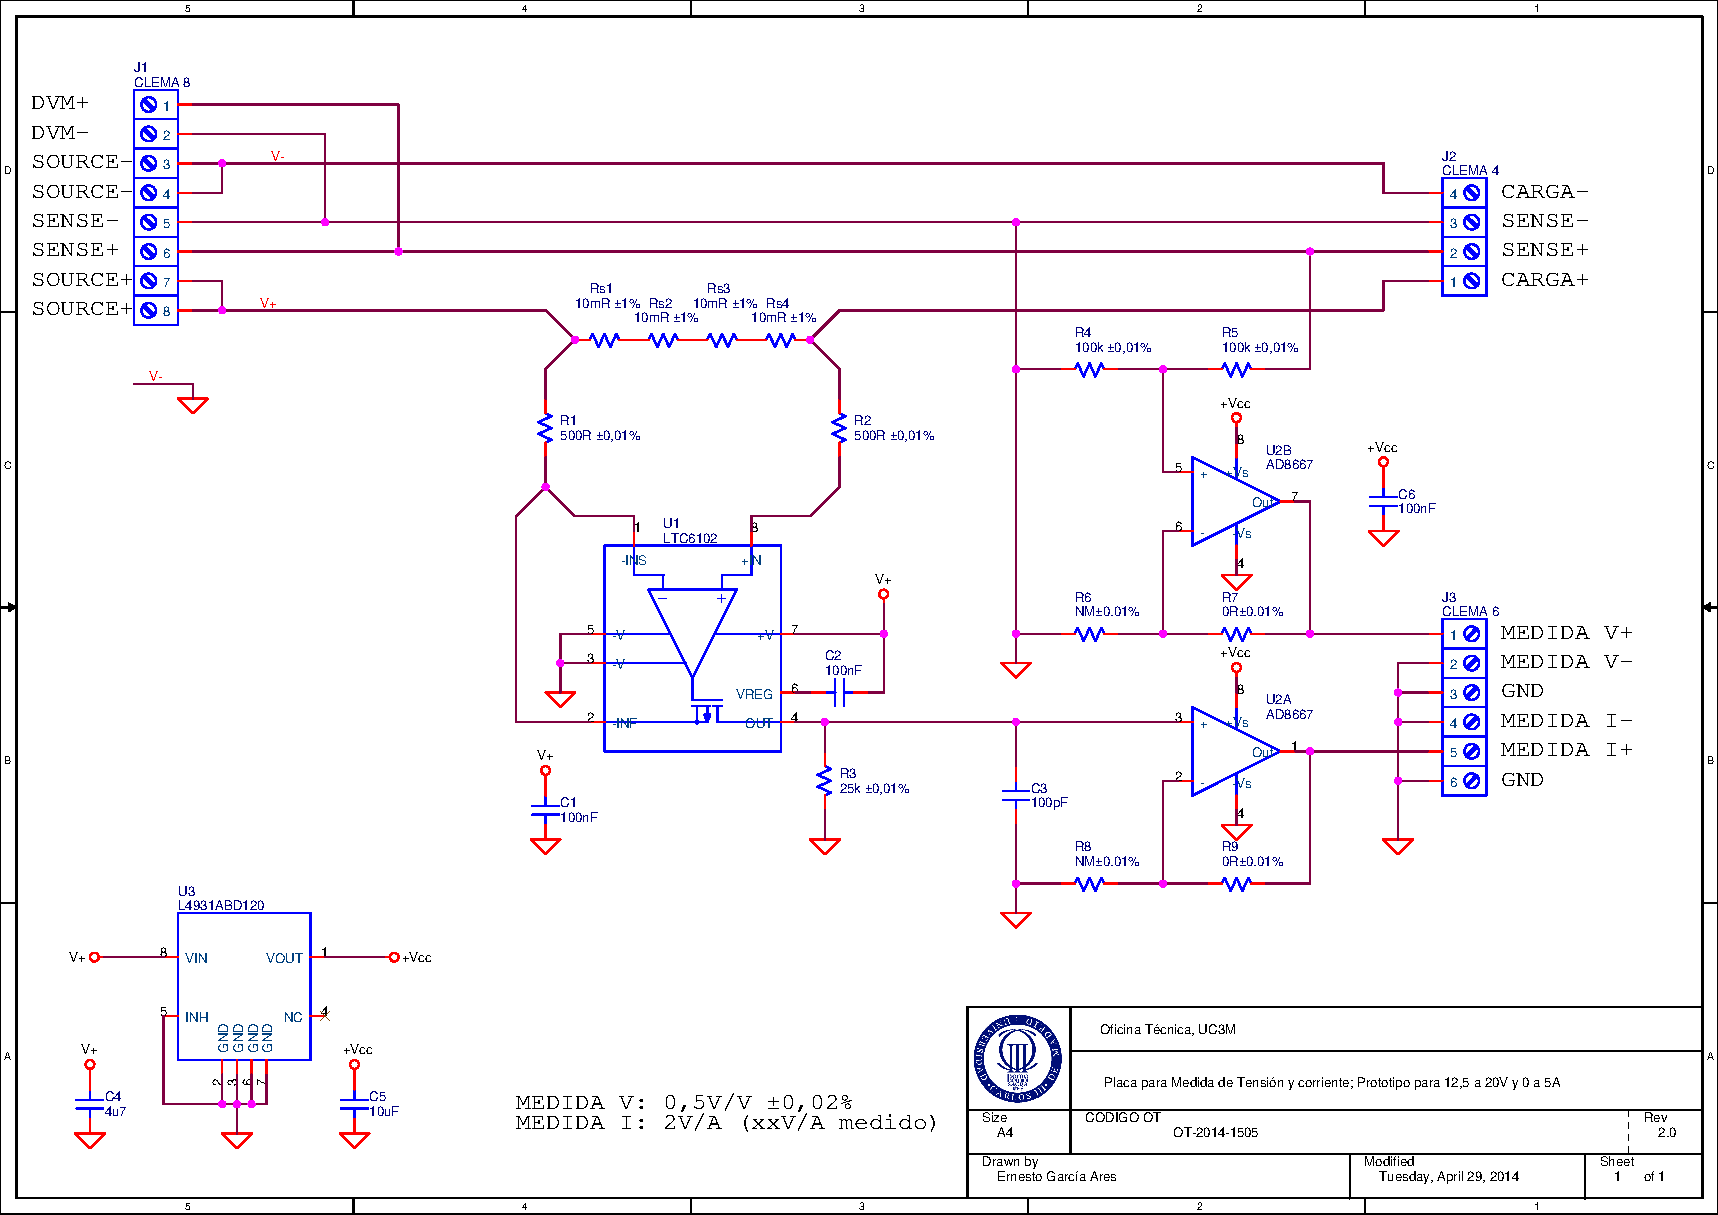
\includegraphics{img/03/schematic-v2} 

}

\caption[12.5-20 V and 0-5 A (100 W max.) prototype.]{12.5-20 V and 0-5 A (100 W max.) prototype.}\label{fig:schematicv2}
\end{sidewaysfigure}



\begin{sidewaysfigure}

{\centering \includegraphics{img/03/schematic-v3} 

}

\caption[0-5 V and 0-2 A (10 W max.) prototype.]{0-5 V and 0-2 A (10 W max.) prototype.}\label{fig:schematicv3}
\end{sidewaysfigure}

\restorewidth

\hypertarget{experimental-validation-of-ra-tpc-inefficiencies}{%
\chapter{Experimental Validation of RA-TPC
Inefficiencies}\label{experimental-validation-of-ra-tpc-inefficiencies}}

\newthought{This appendix} is devoted to experimentally validate the
results from the numerical analysis developed in Chapter \ref{ch:06}. To
this aim, we describe our experimental setup and validation procedure,
first specifying the methodology and then the results achieved.

\hypertarget{experimental-setup}{%
\section{Experimental Setup}\label{experimental-setup}}

We deployed the testbed illustrated in Figure \ref{fig:testbedexp},
which is a variation of the one depicted in Section
\ref{per-component-measurements}, Figure \ref{fig:testbed-card}. It
consists of a station (STA) transmitting evenly-spaced maximum-sized UDP
packets to an access point (AP), an x86-based Alix6f2 board with a
Atheros AR9220 wireless card, running kernel version 3.16.7 and the
\texttt{ath9k} driver. The STA is a desktop PC with a Mini PCI Express
Qualcomm Atheros QCA9880 wireless network adapter, running Fedora Linux
23 with kernel version 4.2.5 and the \texttt{ath10k} driver\footnote{Following
  the discussion on Section
  \ref{sensitivity-to-energy-parameter-scaling} the device's
  cross-factor is not involved in the trade-off, thus we will expect to
  reproduce it by measuring the wireless interface alone.}. We also
installed at the STA a Mini PCI Qualcomm Atheros AR9220 wireless network
adapter to monitor the wireless channel.



\begin{figure}

{\centering \includegraphics{img/06/testbed} 

}

\caption[Experimental setup.]{Experimental setup.}\label{fig:testbedexp}
\end{figure}

As Figure \ref{fig:testbedexp} illustrates, the STA is located in an
office space and the AP is placed in a laboratory 15 m away, and
transmitted frames have to transverse two thin brick walls. The wireless
card uses only one antenna and a practically-empty channel in the 5-GHz
band. Throughout the experiments, the STA is constantly backlogged with
data to send to the AP, and measures the throughput obtained by counting
the number of acknowledgements (ACKs) received.

\hypertarget{methodology-and-results}{%
\section{Methodology and Results}\label{methodology-and-results}}

In order to validate our results, our aim is to replicate the
qualitative behaviour of Figure \ref{fig:efficiency-goodput}, in which
there are energy efficiency ``drops'' as the optimal goodput increases.
However, in our experimental setting, channel conditions are not
controllable, which introduces a notable variability in the results as
it affects both the \(x\)-axis (goodput) and the \(y\)-axis (energy
efficiency). To reduce the impact of this variability, we decided to
change the variable in the \(x\)-axis from the optimal goodput to the
transmission power ---a variable that can be directly configured in the
wireless card---. In this way, the qualitative behaviour to replicate is
the one illustrated in Figure \ref{fig:efficiency-txp}, where we can
still identify the performance ``drops'' causing the loss in energy
efficiency.




\begin{figure}

{\centering \includegraphics{11-appendix-ratpc_files/figure-latex/efficiency-txp-1} 

}

\caption[Energy Efficiency vs.~Transmission Power under
fixed channel conditions for the Raspberry Pi case.]{Energy Efficiency vs.~Transmission Power under
fixed channel conditions for the Raspberry Pi case.}\label{fig:efficiency-txp}
\end{figure}

Building on Figure \ref{fig:efficiency-txp}, we perform a sweep through
all available combinations of MCS (see Table \ref{tab:modes}) and
TXP.\footnote{The model explores a range between 0 and 30 dBm to get the
  big picture, but this particular wireless card only allows us to sweep
  from 0 to 20 dBm.} Furthermore, we also tested two different
configurations of the AP's TXP at different times of the day, to confirm
that this qualitative behaviour is still present under different channel
conditions. For each configuration, we performed 2-second experiments in
which we measure the total bytes successfully sent and the energy
consumed by the QCA9880 card with sub-microsecond precision, and we
compute the energy efficiency achieved for each experiment.




\begin{figure*}

{\centering \includegraphics{11-appendix-ratpc_files/figure-latex/efficiency-txp-exp-1} 

}

\caption[Experimental study of Figure
\ref{fig:efficiency-txp} for two AP configurations.]{Experimental study of Figure
\ref{fig:efficiency-txp} for two AP configurations.}\label{fig:efficiency-txp-exp}
\end{figure*}

The results are shown in Figure \ref{fig:efficiency-txp-exp}. Each graph
corresponds to a different TXP value configured at the AP, and depicts a
single run (note that we performed several runs throughout the day and
found no major qualitative differences across them). Each line type
represents the STA's mode that achieved the highest goodput for each TXP
interval, therefore in some cases low modes do not appear because a
higher mode achieved a higher goodput. Despite the inherent experimental
difficulties, namely, the low granularity of 1-dBm steps and the random
variability of the channel, the experimental results validate the
analytical ones, as the qualitative behaviour of both graphs follows the
one illustrated in Figure \ref{fig:efficiency-txp}. In particular, the
performance ``drops'' of each dominant mode can be clearly observed
(especially for the 36, 48 and 54 Mbps MCSs) despite the variability in
the results.

\hypertarget{performance-evaluation-of-simmer}{%
\chapter{\texorpdfstring{Performance Evaluation of
\texttt{simmer}}{Performance Evaluation of simmer}}\label{performance-evaluation-of-simmer}}

\newthought{This appendix} investigates the performance of
\texttt{simmer} with the aim of assessing its usability as a
general-purpose DES framework. A first section is devoted to measuring
the simulation time of a simple model relative to
\texttt{SimPy}\cite[0pt]{SimPy}\marginnote{\hypersetup{hidelinks}\color{white}\citet{SimPy}}
and
\texttt{SimJulia}\cite[0pt]{GitHub:SimJulia}\marginnote{\hypersetup{hidelinks}\color{white}\citet{GitHub:SimJulia}}.
The reader may find interesting to compare the expressiveness of each
framework. Last but not least, the final section explores the cost of
calling R from C++, revealing the existent trade-off, inherent to the
design of this package, between performance and model complexity.

All the subsequent tests were performed under Fedora Linux 25 running on
an Intel Core2 Quad CPU Q8400, with R 3.3.3, Python 2.7.13,
\texttt{SimPy} 3.0.9, Julia 0.5.1 and \texttt{SimJulia} 0.3.14 from the
default repositories. Absolute execution times presented here are
specific to this platform and configuration, and thus they should not be
taken as representative for any other system. Instead, the relative
performance should be approximately constant across different systems.

\hypertarget{comparison-with-similar-frameworks}{%
\section{Comparison with Similar
Frameworks}\label{comparison-with-similar-frameworks}}

A significant effort has been put into the design of \texttt{simmer} in
order to make it performant enough to run general and relatively large
simulation models in a reasonable amount of time. In this regard, a
relevant comparison can be made against other general-purpose DES
frameworks such as \texttt{SimPy} and \texttt{SimJulia}. To this effect,
we simulate a simple M/M/1 queueing system as follows:

\begin{Shaded}
\begin{Highlighting}[]
\KeywordTok{library}\NormalTok{(}\StringTok{"simmer"}\NormalTok{)}

\NormalTok{test_mm1_simmer <-}\StringTok{ }\ControlFlowTok{function}\NormalTok{(n, m, }\DataTypeTok{mon=}\OtherTok{FALSE}\NormalTok{) \{}
\NormalTok{  mm1 <-}\StringTok{ }\KeywordTok{trajectory}\NormalTok{() }\OperatorTok
\StringTok{    }\KeywordTok{seize}\NormalTok{(}\StringTok{"server"}\NormalTok{, }\DecValTok{1}\NormalTok{) }\OperatorTok
\StringTok{    }\KeywordTok{timeout}\NormalTok{(}\ControlFlowTok{function}\NormalTok{() }\KeywordTok{rexp}\NormalTok{(}\DecValTok{1}\NormalTok{, }\FloatTok{1.1}\NormalTok{)) }\OperatorTok
\StringTok{    }\KeywordTok{release}\NormalTok{(}\StringTok{"server"}\NormalTok{, }\DecValTok{1}\NormalTok{)}

\NormalTok{  env <-}\StringTok{ }\KeywordTok{simmer}\NormalTok{() }\OperatorTok
\StringTok{    }\KeywordTok{add_resource}\NormalTok{(}\StringTok{"server"}\NormalTok{, }\DecValTok{1}\NormalTok{, }\DataTypeTok{mon=}\NormalTok{mon) }\OperatorTok
\StringTok{    }\KeywordTok{add_generator}\NormalTok{(}\StringTok{"customer"}\NormalTok{, mm1, }\ControlFlowTok{function}\NormalTok{() }\KeywordTok{rexp}\NormalTok{(m, }\DecValTok{1}\NormalTok{), }\DataTypeTok{mon=}\NormalTok{mon) }\OperatorTok
\StringTok{    }\KeywordTok{run}\NormalTok{(}\DataTypeTok{until=}\NormalTok{n)}
\NormalTok{\}}
\end{Highlighting}
\end{Shaded}

With the selected arrival rate, \(\lambda=1\), this test simulates an
average of \texttt{n} arrivals entering a nearly saturated system
(\(\rho=1/1.1\)). Given that \texttt{simmer} generators are able to
create arrivals in batches (i.e., more than one arrival for each
function call) for improved performance, the parameter \texttt{m}
controls the size of the batch. Finally, the \texttt{mon} flag enables
or disables monitoring.

Let us build now the equivalent model using \texttt{SimPy}, with base
Python for random number generation. We prepare the Python benchmark
from R using the \texttt{rPython}
package\cite[0pt]{CRAN:rPython}\marginnote{\hypersetup{hidelinks}\color{white}\citet{CRAN:rPython}}
as follows:

\begin{Shaded}
\begin{Highlighting}[]
\NormalTok{rPython}\OperatorTok{::}\KeywordTok{python.exec}\NormalTok{(}\StringTok{"}
\StringTok{import simpy, random, time}

\StringTok{def test_mm1(n):}
\StringTok{  def exp_source(env, lambd, server, mu):}
\StringTok{      while True:}
\StringTok{          dt = random.expovariate(lambd)}
\StringTok{          yield env.timeout(dt)}
\StringTok{          env.process(customer(env, server, mu))}

\StringTok{  def customer(env, server, mu):}
\StringTok{      with server.request() as req:}
\StringTok{          yield req}
\StringTok{          dt = random.expovariate(mu)}
\StringTok{          yield env.timeout(dt)}

\StringTok{  env = simpy.Environment()}
\StringTok{  server = simpy.Resource(env, capacity=1)}
\StringTok{  env.process(exp_source(env, 1, server, 1.1))}
\StringTok{  env.run(until=n)}

\StringTok{def benchmark(n, times):}
\StringTok{  results = []}
\StringTok{  for i in range(0, times):}
\StringTok{    start = time.time()}
\StringTok{    test_mm1(n)}
\StringTok{    results.append(time.time() - start)}
\StringTok{  return results}
\StringTok{"}\NormalTok{)}
\end{Highlighting}
\end{Shaded}

Equivalently, this can be done for \texttt{SimJulia} using the
\texttt{rjulia}
package\cite[0pt]{GitHub:rJulia}\marginnote{\hypersetup{hidelinks}\color{white}\citet{GitHub:rJulia}}.
Once more, \texttt{n} controls the average number of arrivals:

\begin{Shaded}
\begin{Highlighting}[]
\NormalTok{rjulia}\OperatorTok{::}\KeywordTok{julia_init}\NormalTok{()}
\NormalTok{rjulia}\OperatorTok{::}\KeywordTok{julia_void_eval}\NormalTok{(}\StringTok{"}
\StringTok{using SimJulia, Distributions}

\StringTok{function test_mm1(n::Float64)}
\StringTok{  function exp_source(env::Environment, lambd::Float64,}
\StringTok{                      server::Resource, mu::Float64)}
\StringTok{    while true}
\StringTok{      dt = rand(Exponential(1/lambd))}
\StringTok{      yield(Timeout(env, dt))}
\StringTok{      Process(env, customer, server, mu)}
\StringTok{    end}
\StringTok{  end}

\StringTok{  function customer(env::Environment, server::Resource, mu::Float64)}
\StringTok{    yield(Request(server))}
\StringTok{    dt = rand(Exponential(1/mu))}
\StringTok{    yield(Timeout(env, dt))}
\StringTok{    yield(Release(server))}
\StringTok{  end}

\StringTok{  env = Environment()}
\StringTok{  server = Resource(env, 1)}
\StringTok{  Process(env, exp_source, 1.0, server, 1.1)}
\StringTok{  run(env, n)}
\StringTok{end}

\StringTok{function benchmark(n::Float64, times::Int)}
\StringTok{  results = Float64[]}
\StringTok{  test_mm1(n)}
\StringTok{  for i = 1:times}
\StringTok{    push!(results, @elapsed test_mm1(n))}
\StringTok{  end}
\StringTok{  return(results)}
\StringTok{end}
\StringTok{"}\NormalTok{)}
\end{Highlighting}
\end{Shaded}

It can be noted that in both cases there is no monitoring involved,
because either \texttt{SimPy} nor \texttt{SimJulia} provide automatic
monitoring as \texttt{simmer} does. Furthermore, the resulting code for
\texttt{simmer} is more concise and expressive than the equivalent ones
for \texttt{SimPy} and \texttt{SimJulia}, which are very similar.

We obtain the reference benchmark with \texttt{n=1e4} and 20 replicas
for both packages as follows:

\begin{Shaded}
\begin{Highlighting}[]
\NormalTok{n <-}\StringTok{ }\FloatTok{1e4}\NormalTok{L}
\NormalTok{times <-}\StringTok{ }\DecValTok{20}

\NormalTok{ref <-}\StringTok{ }\KeywordTok{data.frame}\NormalTok{(}
  \DataTypeTok{SimPy =}\NormalTok{ rPython}\OperatorTok{::}\KeywordTok{python.call}\NormalTok{(}\StringTok{"benchmark"}\NormalTok{, n, times),}
  \DataTypeTok{SimJulia =}\NormalTok{ rjulia}\OperatorTok{::}\KeywordTok{j2r}\NormalTok{(}\KeywordTok{paste0}\NormalTok{(}\StringTok{"benchmark("}\NormalTok{, n, }\StringTok{".0, "}\NormalTok{, times, }\StringTok{")"}\NormalTok{))}
\NormalTok{)}
\end{Highlighting}
\end{Shaded}

As a matter of fact, we also tested a small DES skeleton in pure R
provided in \citet[s. 7.8.3]{Matloff:2011:ARP:2090080}. This code was
formalised into an R package called \texttt{DES}, available on
GitHub\footnote{\url{https://github.com/matloff/des}} since 2014. The
original code implemented the event queue as an ordered vector which was
updated by performing a binary search. Thus, the execution time of this
version was two orders of magnitude slower than the other frameworks.
The most recent version on GitHub (as of 2017) takes another clever
approach though: it supposes that the event vector will be short and
approximately ordered; therefore, the event vector is not sorted
anymore, and the next event is found using a simple linear search. These
assumptions hold for many cases, and particularly for this M/M/1
scenario. As a result, the performance of this model is only \(\sim2.2\)
times slower than \texttt{SimPy}. Still, it is clear that pure R cannot
compete with other languages in discrete-event simulation, and
\texttt{DES} is not considered in our comparisons hereafter.

Finally, we set a benchmark for \texttt{simmer} using the
\texttt{microbenchmark}
package\cite[0pt]{CRAN:microbenchmark}\marginnote{\hypersetup{hidelinks}\color{white}\citet{CRAN:microbenchmark}},
again with \texttt{n=1e4} and 20 replicas for each test. Figure
\ref{fig:performance-mm1} (left) shows the output of this benchmark.
\texttt{simmer} is tested both in monitored and in non-monitored mode.
The results show that the performance of \texttt{simmer} is equivalent
to \texttt{SimPy} and \texttt{SimJulia}. The non-monitored
\texttt{simmer} shows a slightly better performance than these
frameworks, while the monitored \texttt{simmer} shows a slightly worse
performance.





\begin{figure*}

{\centering \includegraphics[width=0.49\linewidth]{12-appendix-simmer-eval_files/figure-latex/performance-mm1-1} \includegraphics[width=0.49\linewidth]{12-appendix-simmer-eval_files/figure-latex/performance-mm1-2} 

}

\caption[Performance comparison. Boxplots for 20 runs of
the M/M/1 test with \texttt{n=1e4} (left). Performance evolution with
the batch size \(m\) (right).]{Performance comparison. Boxplots for 20 runs of
the M/M/1 test with \texttt{n=1e4} (left). Performance evolution with
the batch size \(m\) (right).}\label{fig:performance-mm1}
\end{figure*}

At this point, it is worth highlighting \texttt{simmer}'s ability to
generate arrivals in batches (hence parameter \(m\)). To better
understand the impact of batched arrival generation, the benchmark was
repeated over a range of \(m\) values \((1, \ldots, 100)\). The results
of the batched arrival generation runs are shown in Figure
\ref{fig:performance-mm1} (right). This plot depicts the average
execution time of the \texttt{simmer} model with (red) and without
(blue) monitoring as a function of the generator batch size \(m\). The
black dashed line sets the average execution time of the \texttt{SimPy}
model to serve as a reference.

The performance with \texttt{m=1} corresponds to what has been shown in
Figure \ref{fig:performance-mm1} (left). But as \(m\) increases,
\texttt{simmer} performance quickly improves and becomes \(\sim1.6\) to
\(1.9\) times faster than \texttt{SimPy}. Surprisingly, there is no
additional gain with batches greater than 40-50 arrivals at a time, but
there is no penalty either with bigger batches. Therefore, it is always
recommended to generate arrivals in big batches whenever possible.

\hypertarget{the-cost-of-calling-r-from-c}{%
\section{The Cost of Calling R from
C++}\label{the-cost-of-calling-r-from-c}}

The C++ simulation core provided by \texttt{simmer} is quite fast, as we
have demonstrated, but performance is adversely affected by numerous
calls to R. The practice of calling R from C++ is generally strongly
discouraged due to the overhead involved. However, in the case of
\texttt{simmer}, it not only makes sense, but is even fundamental in
order to provide the user with enough flexibility to build all kinds of
simulation models. Nevertheless, this cost must be known, and taken into
account whenever a higher performance is needed.

To explore the cost of calling R from C++, let us define the following
test:

\begin{Shaded}
\begin{Highlighting}[]
\KeywordTok{library}\NormalTok{(}\StringTok{"simmer"}\NormalTok{)}

\NormalTok{test_simmer <-}\StringTok{ }\ControlFlowTok{function}\NormalTok{(n, delay) \{}
\NormalTok{  test <-}\StringTok{ }\KeywordTok{trajectory}\NormalTok{() }\OperatorTok
\StringTok{    }\KeywordTok{timeout}\NormalTok{(delay)}

\NormalTok{  env <-}\StringTok{ }\KeywordTok{simmer}\NormalTok{() }\OperatorTok
\StringTok{    }\KeywordTok{add_generator}\NormalTok{(}\StringTok{"test"}\NormalTok{, test, }\KeywordTok{at}\NormalTok{(}\DecValTok{1}\OperatorTok{:}\NormalTok{n)) }\OperatorTok
\StringTok{    }\KeywordTok{run}\NormalTok{(}\OtherTok{Inf}\NormalTok{)}

\NormalTok{  arrivals <-}\StringTok{ }\KeywordTok{get_mon_arrivals}\NormalTok{(env)}
\NormalTok{\}}
\end{Highlighting}
\end{Shaded}

\pagebreak

This toy example performs a very simple simulation in which \texttt{n}
arrivals are attached (in one shot, thanks to the convenience function
\texttt{at()}) to a \texttt{test} trajectory at \(t=1, 2, ..., n\). The
trajectory consists of a single activity: a timeout with some
configurable \texttt{delay} that may be a fixed value or a function
call. Finally, after the simulation, the monitored data is extracted
from the simulation core to R. Effectively, this is equivalent to
generating a data frame of \texttt{n} rows (see the example output in
Table \ref{tab:test-simmer-output-table}).




\begin{table}

\begin{center}
\resizebox{\linewidth}{!}{
\begin{tabular}{rrrrrr}
\toprule
Name & Start time & End time & Activity time & Finished & Replication\\
\midrule
test0 & 1 & 2 & 1 & TRUE & 1\\
test1 & 2 & 3 & 1 & TRUE & 1\\
test2 & 3 & 4 & 1 & TRUE & 1\\
\bottomrule
\end{tabular}}
\end{center}
\caption{\label{tab:test-simmer-output-table}Output from the \texttt{test\_simmer()}
function.}
\end{table}

As a matter of comparison, the following \texttt{test\_R\_for()}
function produces the very same data using base R:

\begin{Shaded}
\begin{Highlighting}[]
\NormalTok{test_R_for <-}\StringTok{ }\ControlFlowTok{function}\NormalTok{(n) \{}
\NormalTok{  name <-}\StringTok{ }\KeywordTok{character}\NormalTok{(n)}
\NormalTok{  start_time <-}\StringTok{ }\KeywordTok{numeric}\NormalTok{(n)}
\NormalTok{  end_time <-}\StringTok{ }\KeywordTok{numeric}\NormalTok{(n)}
\NormalTok{  activity_time <-}\StringTok{ }\KeywordTok{logical}\NormalTok{(n)}
\NormalTok{  finished <-}\StringTok{ }\KeywordTok{numeric}\NormalTok{(n)}

  \ControlFlowTok{for}\NormalTok{ (i }\ControlFlowTok{in} \DecValTok{1}\OperatorTok{:}\NormalTok{n) \{}
\NormalTok{    name[i] <-}\StringTok{ }\KeywordTok{paste0}\NormalTok{(}\StringTok{"test"}\NormalTok{, i}\DecValTok{-1}\NormalTok{)}
\NormalTok{    start_time[i] <-}\StringTok{ }\NormalTok{i}
\NormalTok{    end_time[i] <-}\StringTok{ }\NormalTok{i}\OperatorTok{+}\DecValTok{1}
\NormalTok{    activity_time[i] <-}\StringTok{ }\DecValTok{1}
\NormalTok{    finished[i] <-}\StringTok{ }\OtherTok{TRUE}
\NormalTok{  \}}

\NormalTok{  arrivals <-}\StringTok{ }\KeywordTok{data.frame}\NormalTok{(}
    \DataTypeTok{name=}\NormalTok{name,}
    \DataTypeTok{start_time=}\NormalTok{start_time,}
    \DataTypeTok{end_time=}\NormalTok{end_time,}
    \DataTypeTok{activity_time=}\NormalTok{activity_time,}
    \DataTypeTok{finished=}\NormalTok{finished,}
    \DataTypeTok{replication =} \DecValTok{1}
\NormalTok{  )}
\NormalTok{\}}
\end{Highlighting}
\end{Shaded}

Note that we are using a \texttt{for} loop to mimic the behaviour of
\texttt{simmer}'s internals, of how monitoring is made, but we concede
the advantage of pre-allocated vectors to R. A second base R
implementation, which builts upon the \texttt{lapply()} function, is
implemented as the \texttt{test\_R\_lapply()} function:

\begin{Shaded}
\begin{Highlighting}[]
\NormalTok{test_R_lapply <-}\StringTok{ }\ControlFlowTok{function}\NormalTok{(n) \{}
  \KeywordTok{as.data.frame}\NormalTok{(}\KeywordTok{do.call}\NormalTok{(rbind, }\KeywordTok{lapply}\NormalTok{(}\DecValTok{1}\OperatorTok{:}\NormalTok{n, }\ControlFlowTok{function}\NormalTok{(i) \{}
    \KeywordTok{list}\NormalTok{(}
      \DataTypeTok{name =} \KeywordTok{paste0}\NormalTok{(}\StringTok{"test"}\NormalTok{, i }\OperatorTok{-}\StringTok{ }\DecValTok{1}\NormalTok{),}
      \DataTypeTok{start_time =}\NormalTok{ i,}
      \DataTypeTok{end_time =}\NormalTok{ i }\OperatorTok{+}\StringTok{ }\DecValTok{1}\NormalTok{,}
      \DataTypeTok{activity_time =} \DecValTok{1}\NormalTok{,}
      \DataTypeTok{finished =} \OtherTok{TRUE}\NormalTok{,}
      \DataTypeTok{replication =} \DecValTok{1}
\NormalTok{    )}
\NormalTok{  \})))}
\NormalTok{\}}
\end{Highlighting}
\end{Shaded}

The \texttt{test\_simmer()}, \texttt{test\_R\_for()} and
\texttt{test\_R\_lapply()} functions all produce exactly the same data
in a similar manner (cfr. Table \ref{tab:test-simmer-output-table}).
Now, we want to compare how a delay consisting of a function call
instead of a fixed value impacts the performance of \texttt{simmer}, and
we use \texttt{test\_R\_for()} and \texttt{test\_R\_lapply()} as
yardsticks.

The benchmark was executed with \texttt{n=1e5} and 20 replicas for each
test. Table \ref{tab:performance-table} shows a summary of the resulting
timings.

\begin{table}

\begin{center}
\resizebox{\linewidth}{!}{
\begin{tabular}{>{\ttfamily}rrrrr}
\toprule
Expr & Min & Mean & Median & Max\\
\midrule
test\_simmer(n, 1) & 429.8663 & 492.365 & 480.5408 & 599.3547\\
test\_simmer(n, function() 1) & 3067.9957 & 3176.963 & 3165.6859 & 3434.7979\\
test\_R\_for(n) & 2053.0840 & 2176.164 & 2102.5848 & 2438.6836\\
test\_R\_lapply(n) & 1525.6682 & 1754.028 & 1757.7566 & 2002.6634\\
\bottomrule
\end{tabular}}
\end{center}
\caption{\label{tab:performance-table}Execution time (milliseconds).}
\end{table}

As we can see, \texttt{simmer} is \(\sim4.4\) times faster than
\texttt{for}-based base R and \(\sim3.6\) times faster than
\texttt{lapply}-based base R on average when we set a fixed delay. On
the ther hand, if we replace it for a function call, the execution
becomes \(\sim6.5\) times slower, or \(\sim1.5\) times slower than
\texttt{for}-based base R. It is indeed a quite good result if we take
into account the fact that base R pre-allocates memory, and that
\texttt{simmer} is doing a lot more internally. But still, these results
highlight the overheads involved and encourage the use of fixed values
instead of function calls whenever possible.

\backmatter
\fancyhead[RO]{\smallcaps{\newlinetospace{References}}\quad\thepage}

\bibliography{thesis.bib,packages.bib}


%\cleardoublepage
%\fancyhead[RO]{\smallcaps{\newlinetospace{Index}}\quad\thepage}
%\phantomsection
%\printindex
\newpage\thispagestyle{empty}\mbox{}
\includepdf{img/cover-back.pdf}

\end{document}
